\documentclass{workbook}

\newcommand{\copyrightdate}{2024}

\usepackage{ifxetex}
\usepackage[utf8]{inputenc}
\usepackage{hyperref}
\usepackage{hyperxmp} % Embed meta data into the PDF
\hypersetup{%
	hidelinks=true,
	linkcolor = {0 0 1},
	% Metadata to be embedded by hyperxmp
	pdftitle={Ordinary Differential Equations (\jobname)},
	pdfauthor={Bernardo Galv\~ao-Sousa, Jason Siefken},
	pdfauthortitle={Author},
	pdfcopyright={Copyright (C) \copyrightdate, Bernardo Galv\~ao-Sousa, Jason Siefken},
	pdfsubject={Ordinary Differential Equations textbook/workbook},
	pdfkeywords={ordinary differential equations, ODEs, modeling, vectors, mathematics, textbook},
	pdfurl={https://github.com/siefkenj/IBLODEs/},
	pdflicenseurl={https://creativecommons.org/licenses/by-sa/4.0/},
}

%%%
% import all needed packages and macros
%%%
\usepackage[yyyymmdd]{datetime}
%%
%% All packages and macros needed for the problemsets
%%

\usepackage{amsmath}

\usepackage{lipsum}
%\usepackage{showframe}
%\usepackage{layout}


\usepackage[charter,cal=cmcal]{mathdesign} %different font
%\usepackage{avant}

\usepackage{microtype}
\usepackage{mathtools}
\usepackage{etoolbox}
%\usepackage{amsfonts}
%\usepackage{amssymb}
\usepackage{graphicx}
\graphicspath{{images/}}
\usepackage[inline]{enumitem}
\usepackage{xparse}
\usepackage{ifthen}
\usepackage{caption}
\usepackage{subcaption}
\usepackage{tikz}
	\usetikzlibrary{fit}
	\usetikzlibrary{fadings}
	\usetikzlibrary{calc}
	\tikzset{>=latex}
	\usetikzlibrary{cd}
	\usetikzlibrary{spy}
	\usetikzlibrary{patterns}
	\usetikzlibrary{decorations, decorations.pathreplacing, decorations.markings}

\usepackage{fancyhdr}
\usepackage{calc}
\usepackage{wrapfig}
\usepackage{marginnote}
\usepackage{mparhack}
\usepackage{marginfix}
\usepackage{indextools}
\usepackage[open=false]{bookmark}  % render the pdf TOC in the proper order
\hypersetup{
	hidelinks=true,
	linkcolor = {0 0 1},
	unicode=true,
	psdextra=true,
}
\usepackage{common/nicematrix}

%\usepackage[
%  linktocpage=false,      % no page numbers are clickable
%  colorlinks=false,       % no color
%  breaklinks=true,        % break URLs
%  bookmarks,              % creates bookmarks in pdf
%  hyperfootnotes=true,    % clickable footnotes
%  pdfborder={0 0 0},      % for removing borders around links
%  bookmarksnumbered=true, % If Acrobat bookmarks are requested, include section numbers.
%  bookmarksopen=false,    % If Acrobat bookmarks are requested, show them with all the subtrees expanded.
%  %hidelinks=true,
%  %linkcolor=blue,
%  %citecolor=blue,
%  %urlcolor=blue,
%  pdfpagemode={UseOutlines}, % show pdf bookmarks (indices) on startup; does not function all the time
%  pdftitle={...}, % title
%  pdfauthor={...}, % author
%  pdfkeywords={...}, % subject of the document
%  pdfsubject={...}, % list of keywords
%  pdfmenubar=true,        % make PDF viewer’s menu bar visible
%  pdfpagelabels,
%]{hyperref}
%\usepackage[hidelinks,]{hyperref}
\usepackage{fnpct} % fancy footnote spacing
\usepackage{bm}
\usepackage{systeme}
\usepackage{datatool}% http://ctan.org/pkg/datatool for sorted lists
\usepackage{xspace}


\usepackage{pgfplots}
\pgfplotsset{compat=1.16}
	\usepgfplotslibrary{fillbetween}
%%%
% Useful Linear Algebra macros
%%%
\newcommand{\declarecommand}[1]{\providecommand{#1}{}\renewcommand{#1}}
\DeclareDocumentCommand{\R}{}{\mathbb{R}}  % we don't care if it's already defined.  We really want *this* command!
\DeclareDocumentCommand{\Z}{}{\mathbb{Z}}
\DeclareDocumentCommand{\Q}{}{\mathbb{Q}}
\DeclareDocumentCommand{\N}{}{\mathbb{N}}
\DeclareDocumentCommand{\C}{}{\mathbb{C}}
\DeclareDocumentCommand{\d}{}{\mathrm{d}}
\DeclareDocumentCommand{\dd}{}{\mathbbm{d}} % exterior derivative
\DeclareMathOperator{\Span}{span}
\DeclareMathOperator{\Img}{img}
\DeclareMathOperator{\Id}{id}
\DeclareMathOperator{\Ident}{\Id}
\DeclareMathOperator{\Vol}{Vol}
\DeclareMathOperator{\VolChange}{Vol\hspace{1.5pt}Change}
\DeclareMathOperator{\Range}{range}
\DeclareMathOperator{\Rref}{rref}
\DeclareMathOperator{\Rank}{rank}
\DeclareMathOperator{\Comp}{\Vcomp}
\DeclareMathOperator{\Vcomp}{v\hspace{1pt}comp}
\DeclareMathOperator{\Null}{null}
\DeclareMathOperator{\Nullity}{nullity}
\DeclareMathOperator{\Char}{char}
\DeclareMathOperator{\Proj}{proj}
\DeclareMathOperator{\Flux}{Flux}
\DeclareMathOperator{\Circ}{Circ}
\DeclareMathOperator{\chr}{char}
\DeclareMathOperator{\Dim}{dim}
\DeclareMathOperator{\Perp}{perp}
\DeclareMathOperator{\Ker}{kernel}
\DeclareMathOperator{\Row}{row}
\DeclareMathOperator{\Col}{col}
\DeclareMathOperator{\Rep}{Rep}
\newcommand{\BasisChange}[2]{[#2\!\leftarrow\!#1]}
\newcommand{\proj}{\Proj}
\newcommand{\rref}{\Rref}
\newcommand{\xhat}{{\vec e_1}}
\newcommand{\yhat}{{\vec e_2}}
\newcommand{\zhat}{{\vec e_3}}
\newcommand{\sbasis}[1]{\vec { e}_{#1}}
\newcommand{\mat}[1]{\begin{bmatrix*}[r]#1\end{bmatrix*}}
\newcommand{\matc}[1]{\begin{bmatrix}#1\end{bmatrix}}
\newcommand{\formarg}[2]{\big(#1;\, #2\big)}
\DeclarePairedDelimiter\abs{\lvert}{\rvert}
\DeclarePairedDelimiter\Abs{\lvert}{\rvert}
\DeclarePairedDelimiter\norm{\lVert}{\rVert}
\newcommand{\Norm}[1]{\norm{#1}}
% just to make sure it exists
\providecommand\given{}
% can be useful to refer to this outside \Set
\newcommand\SetSymbol[1][]{%
	\nonscript\::%
	\allowbreak
	\nonscript\:
	\mathopen{}}
\DeclarePairedDelimiterX\Set[1]\{\}{%
	\renewcommand\given{\SetSymbol[\delimsize]}
	#1
}
\newcommand{\Rrefto}{\xrightarrow{\text{row reduces to}}}


% redefine bmatrix,etc to allow optional argument for augmenting
% code from https://tex.stackexchange.com/questions/2233/whats-the-best-way-make-an-augmented-coefficient-matrix
\makeatletter
\renewcommand*\env@matrix[1][*\c@MaxMatrixCols c]{%
  \hskip -\arraycolsep
  \let\@ifnextchar\new@ifnextchar
  \array{#1}}
\makeatother

\newcommand{\scaledgrid}[1]{%
	\begin{tikzpicture}[scale=#1]
		\draw[thin, white!20!black, dotted] (-4.1,-4.1) grid (4.1,4.1);
		\draw[ <->] (-4.3,0) -- (4.3,0);
		\draw[ <->] (0,-4.3) -- (0,4.3);
	\end{tikzpicture}
}
\newcommand{\scaledshortgrid}[1]{%
	\begin{tikzpicture}[scale=#1]
		\draw[thin, white!20!black, dotted] (-4.1,-2.1) grid (4.1,2.1);
		\draw[ <->] (-4.3,0) -- (4.3,0);
		\draw[ <->] (0,-2.3) -- (0,2.3);
	\end{tikzpicture}
}
\newcommand{\singlegrid}{\scaledgrid{1}}
\newcommand{\doublegrid}{\mbox{\scaledgrid{.9}\scaledgrid{.9}}\par}
\newcommand{\triplegrid}{\mbox{\scaledgrid{.6}\scaledgrid{.6}\scaledgrid{.6}}\par}

% labels for source attributions
\NewDocumentCommand{\beezer}{o}{%
	\IfNoValueTF{#1}{%
		{\color{blue}\sffamily{B}}%
	}{%
		{\color{blue}\sffamily{B}}%  XXX Todo, make this href to the appropriate problem number
	}\xspace%
}
\NewDocumentCommand{\hefferon}{o}{%
	\IfNoValueTF{#1}{%
		{\color{blue}\sffamily{H}}%
	}{%
		{\color{blue}\sffamily{H}}%  XXX Todo, make this href to the appropriate problem number
	}\xspace%
}

\DeclareDocumentEnvironment{beforeyouread}{}{
Before you read, make sure you are comfortable with the following.
Please do the ``Quick Check'' problem to see if you are comfortable with each
task.
\begin{itemize}
}{
\end{itemize}
}
\newcommand\quickcheck[1]{\par {\footnotesize \textsc{Quick Check.} \textrm{#1}}}

% Dummy, voidable environments
\DeclareDocumentEnvironment{bookonly}{o}{}{}
\DeclareDocumentEnvironment{displayonly}{o}{}{}

\newcommand{\hdash}{\text{\-------}}
\newcommand{\bigmathstrut}{\vphantom{\Big(}}


\usepackage{breqn}

\usepackage{pdfrender} % For text title

%%%
% Set up the footers to have the correct copyright notices
%%%

\fancypagestyle{siefken}{%
	\rfoot{\footnotesize\it \copyright\,Bernardo Galv\~ao-Sousa \& Jason Siefken, \copyrightdate \ \makebox(30,5){
\includegraphics[height=1.2em]{by-sa.pdf}}}
	\lfoot{}
	\renewcommand{\headrulewidth}{0pt}
}


%%
% Allow hiding of environments
%%
\usepackage{environ}% http://ctan.org/pkg/environ
\makeatletter
\newcommand{\voidenvironment}[1]{%
  \expandafter\providecommand\csname env@#1@save@env\endcsname{}%
  \expandafter\providecommand\csname env@#1@process\endcsname{}%
  \@ifundefined{#1}{}{\RenewEnviron{#1}{}}%
}
\makeatother
% allow pagebreaks that only display in `standard` mode
\newcommand{\displayonlynewpage}{\begin{displayonly}\newpage\end{displayonly}}
% allow pagebreaks that only display in `book` mode
\newcommand{\bookonlynewpage}{\begin{bookonly}\newpage\end{bookonly}}


%
% Set up the three render modes: standard, instructor, and solutions.
% These render with varying amounts of extra data (like solutions and notes)
%
\newtoggle{instructor}
\newtoggle{standard}
\newtoggle{solutions}
\newtoggle{book}
\newtoggle{slides}
\newtoggle{slideswhite}
\newcommand{\setinstructor}{
	\toggletrue{instructor}
	\togglefalse{standard}
	\togglefalse{solutions}
	\togglefalse{book}
	\togglefalse{slides}
	\togglefalse{slideswhite}
}
\newcommand{\setstandard}{
	\togglefalse{instructor}
	\toggletrue{standard}
	\togglefalse{solutions}
	\togglefalse{book}
	\togglefalse{slides}
	\togglefalse{slideswhite}
}
\newcommand{\setsolutions}{
	\togglefalse{instructor}
	\togglefalse{standard}
	\toggletrue{solutions}
	\togglefalse{book}
	\togglefalse{slides}
	\togglefalse{slideswhite}
}
\newcommand{\setbook}{
	\togglefalse{instructor}
	\togglefalse{standard}
	\togglefalse{solutions}
	\toggletrue{book}
	\togglefalse{slides}
	\togglefalse{slideswhite}
}
\newcommand{\setslides}{
	\togglefalse{instructor}
	\togglefalse{standard}
	\togglefalse{solutions}
	\togglefalse{book}
	\toggletrue{slides}
	\togglefalse{slideswhite}
}
\newcommand{\setslideswhite}{
	\togglefalse{instructor}
	\togglefalse{standard}
	\togglefalse{solutions}
	\togglefalse{book}
	\togglefalse{slides}
	\toggletrue{slideswhite}
}


%
% Infer the document level from the \jobname
%
\usepackage{xstring}
\IfSubStr{\jobname}{\detokenize{book}}{\setbook}{
	\IfSubStr{\jobname}{\detokenize{solutions}}{\setsolutions}{
		\IfSubStr{\jobname}{\detokenize{instructor}}{\setinstructor}{
			\IfSubStr{\jobname}{\detokenize{slides}}{\setslides}{
				\IfSubStr{\jobname}{\detokenize{white}}{\setslideswhite}{
						\setstandard
				}
			}
		}
	}
}


\setbookoptions{
	twosided = false,
	inline solutions = false,
}


\NewColoredEnvironment{
	name = lesson,
	display name = Lesson,
	banner color = Plum,
	title color = Plum,
	banner on left = true,
	open right = false,
}
\NewColoredEnvironment{
	name = module,
	display name = Module,
	banner color = Turquoise,
	title color = Cerulean,
	definition color = Cerulean,
	theorem color = myorange,
}
\NewColoredEnvironment{
	name = appendix,
	display name = Appendix,
	banner color = LimeGreen,
	title color = LimeGreen!70!Green!80!black,
	definition color = Cerulean,
	theorem color = myorange,
}
\NewColoredEnvironment{
	name = indices,
	display name = Indices,
	banner color = Green,
	title color = Green,
}
\NewColoredEnvironment{
	name = tutorial,
	display name = Tutorial,
	banner color = Peach,
	title color = Peach!80!black,
	emphbox color = Peach,
	% We will print tutorial worksheets back-to-back to save space
	open right = false,
}




\loadgeometry{default}

%
% Hide the non-problem environments
%
\newcommand{\coversubtitle}{} % we override the subtitle in each mode, so make sure the command exists to override.
\iftoggle{instructor}{
	\voidenvironment{module}
	\voidenvironment{appendix}
	\voidenvironment{bookonly}
	\voidenvironment{displayonly}
	\renewcommand{\coversubtitle}{Instructor Guide}
}{}
\iftoggle{solutions}{
	\voidenvironment{module}
	\voidenvironment{appendix}
	\voidenvironment{bookonly}
	\voidenvironment{displayonly}
	\voidenvironment{lesson}
	\voidenvironment{notes}
	\renewcommand{\coversubtitle}{Solutions}
}{}
\iftoggle{standard}{
	\voidenvironment{module}
	\voidenvironment{appendix}
	\voidenvironment{bookonly}
	\voidenvironment{solution}
	\voidenvironment{annotation}
	\voidenvironment{lesson}
	\renewcommand{\coversubtitle}{MAT244 Notes}
	\loadgeometry{default}
}{}
\iftoggle{book}{
	\voidenvironment{displayonly}
	\voidenvironment{solution}
	\voidenvironment{annotation}
	\voidenvironment{lesson}
	\renewcommand{\coversubtitle}{{\hspace{-5pt}\begin{tabular}{l}MAT244 Workbook\\\small\today{} Edition\end{tabular}}}
	\setbookoptions{
		twosided = true,
		inline solutions = false,
	}
	\loadgeometry{book}
}{}
\iftoggle{slides}{
	\voidenvironment{module}
	\voidenvironment{appendix}
	\voidenvironment{bookonly}
	\voidenvironment{solution}
	\voidenvironment{annotation}
	\voidenvironment{lesson}
	\renewcommand{\coversubtitle}{MAT244 Slides}
	\loadgeometry{slides}
	\initSlides
}{}
\iftoggle{slideswhite}{
	\voidenvironment{module}
	\voidenvironment{appendix}
	\voidenvironment{bookonly}
	\voidenvironment{solution}
	\voidenvironment{annotation}
	\voidenvironment{lesson}
	\renewcommand{\coversubtitle}{\hspace{-70pt}MAT244 Student Slides}
	\loadgeometry{slides}
	\initSlidesWhite
}{}
%\voidenvironment{solution}
%\voidenvironment{annotation}
%\voidenvironment{lesson}
%%\voidenvironment{notes}
%%\voidenvironment{displayonly}

% Allow an index to be created
\makeindex[title=Index of Terms, columns=3]
\makeindex[name=definitions, title=Index of Definitions, columns=3]
\makeindex[name=symbols, title=Index of Symbols, columns=3]

\indexsetup{
	level=\Heading,
	noclearpage
}

\begin{document}
%%
%% Import definitions from definition.tex; all definitions can be restated multiple times
%%

%%
%% Start Definitions (each of these we can reuse)
%%
\begin{SaveDefinition}[
		key=SubsetSuperset,
		title={Subset \& Superset}
	]
	The set $B$ is a \emph{subset}\index[definitions]{Subset} of the set $A$, written $B\subseteq A$\index[symbols]{$\subseteq$}, if for all
	$b\in B$ we also have $b\in A$.  In this case, $A$ is called a \emph{superset}\index[definitions]{Superset}
	of $B$.\footnote{
		Some mathematicians use the symbol $\subset$ instead of $\subseteq$.}
\end{SaveDefinition}
\begin{SaveDefinition}[
		key=SetEquality,
		title={Set Equality}
	]
	The sets $A$ and $B$ are \emph{equal}\index{Set!equality}\index[definitions]{Set!equality}, written $A=B$, if $A\subseteq B$ and $B\subseteq A$.
\end{SaveDefinition}
\begin{SaveDefinition}[
		key=SetSubtraction,
		title={Set Subtraction}
	]
	For sets $A$ and $B$, the \emph{set-wise difference}\index[definitions]{Set!subtraction}\index{Set!subtraction} between $A$ and $B$,
	written $A\backslash B$, is the set
	\[
		A\backslash B = \Set{x\given x\in A\text{ and }x\notin B}.
	\]
\end{SaveDefinition}
\begin{SaveDefinition}[
		key=UnionsIntersections,
		title={Unions \& Intersections}
	]
	Let $X$ and $Y$ be sets. The \emph{union}\index[definitions]{Set!union}\index{Set!union}\index[symbols]{$\cup$} of $X$ and $Y$ and the
	\emph{intersection}\index[definitions]{Set!intersection}\index{Set!intersection}\index[symbols]{$\cap$} of $X$
	and $Y$ are defined as follows.

	\smallskip

	\hfill\begin{minipage}{\dimexpr\textwidth-3cm}
	\begin{itemize}
		\item[(union)] $X\cup Y = \Set{ a \given a\in X\text{ or }a\in Y}$.
		\item[(intersection)] $X\cap Y = \Set{ a \given a\in X\text{ and }a\in Y}$.
	\end{itemize}
	\end{minipage}
\end{SaveDefinition}

\begin{SaveDefinition}[key=Set, title={Set}]
	A \emph{set}\index[definitions]{Set} is a (possibly infinite) collection of items and is notated
	with curly braces (for example, $\{1,2,3\}$ is the set containing the
	numbers 1, 2, and 3). We call the items in a set
	\emph{elements}.

	If $X$ is a set and $a$ is an element of $X$, we may write $a\in X$,
	which is read ``$a$ is an element of $X$.''

	If $X$ is a set, a
	\emph{subset} $Y$ of $X$ (written $Y\subseteq X$) is a set such that
	every element of $Y$ is an element of $X$. Two sets are called
	\emph{equal} if they are subsets of each other (i.e., $X=Y$ if $X\subseteq
	Y$ and $Y\subseteq X$).

	We can define a subset using
	\emph{set-builder notation}. That is, if $X$ is a set, we can define the
	subset
	\[
		Y= \Set*{a\in X \given \text{some rule involving }a},
	\]
	 which is read ``$Y$ is the set of $a$ in $X$ {\bf such that} some rule
	involving $a$ is true.'' If $X$ is intuitive, we may omit it and simply write
	$Y=\{a:\text{some rule involving }a\}$. You may equivalently use ``$|$''
	instead of ``$:$'', writing $Y=\{a\,|\,\text{some rule involving }a\}$.
\end{SaveDefinition}

\begin{SaveDefinition}[key=ZeroVector, title={Zero Vector}]
		The \emph{zero vector}\index{Zero vector ($\vec 0$)}\index[definitions]{Zero vector ($\vec 0$)}, notated as $\vec 0$\index[symbols]{$\vec 0$},
		is the vector with no magnitude.
\end{SaveDefinition}

\begin{SaveDefinition}[key=LinearCombination, title={Linear Combination}]
	A \emph{linear combination}\index{Linear combination}\index[definitions]{Linear combination} of the vectors
	$\vec v_{1},\vec v_{2},\ldots,\vec v_{n}$ is a vector
	\[
		\vec w = \alpha_{1}\vec v_{1}+\alpha_{2}\vec v_{2}+\cdots+\alpha_{n}\vec
		v_{n}.
	\]
	 The scalars $\alpha_{1},\alpha_{2},\ldots,\alpha_{n}$ are called the
	\emph{coefficients}\index{Linear combination!coefficient of}\index[definitions]{Linear combination!coefficient of} of the linear combination.
\end{SaveDefinition}

\begin{SaveDefinition}[
	key=NonnegativeConvexLinearCombinations,
	title={Non-negative \& Convex Linear Combinations}]

	Let
	$\vec w=\alpha_{1}\vec v_{1}+\alpha_{2}\vec v_{2}+\cdots+\alpha_{n}\vec
	v_{n}.$
	The vector $\vec w$ is called a
	\emph{non-negative}\index{Linear combination!non-negative}\index[definitions]{Linear combination!non-negative} linear combination of
	$\vec v_{1},\vec v_{2},\ldots,\vec v_{n}$ if
	\[\alpha_{1},\alpha_{2},\ldots,\alpha_{n}\geq 0.\]

	The vector $\vec w$ is called a
	\emph{convex}\index{Linear combination!convex}\index[definitions]{Linear combination!convex} linear combination of
	$\vec v_{1},\vec v_{2},\ldots,\vec v_{n}$
	if \[\alpha_{1},\alpha_{2},\ldots,\alpha_{n}\geq 0\qquad\text{and}\qquad
	\alpha_{1}+\alpha_{2}+\cdots+\alpha_{n}=1.\]
\end{SaveDefinition}

\begin{SaveDefinition}[key=VectorFormofaLine, title={Vector Form of a Line}]
	Let $\ell$ be a line and let $\vec d$ and $\vec p$ be vectors. If $\ell=\Set{\vec
	x\given \vec x= t\vec d+\vec p\text{ for some } t\in\R }$, we say the vector equation

	\[
		\vec x=t\vec d+\vec p
	\]
	 is $\ell$ expressed in
	\emph{vector form}\index{Line!vector form of}\index[definitions]{Line!vector form of}. The vector $\vec d$ is called a
	\emph{direction vector}\index{Line!direction vector for}\index[definitions]{Line!direction vector for} for $\ell$.
\end{SaveDefinition}

\begin{SaveDefinition}[key=VectorFormofaPlane, title={Vector Form of a Plane}]
	A plane $\mathcal P$ is written in
	\emph{vector form}\index{Plane!vector form of}\index[definitions]{Plane!vector form of} if it is expressed as
	\[
		\vec x=t\vec d_{1} +s\vec d_{2}+\vec p
	\]
	 for some vectors $\vec d_{1}$ and $\vec d_{2}$ and point $\vec p$. That
	is,
	$\mathcal P = \{\vec x: \vec x= t\vec d_{1}+s\vec d_{2} +\vec p\text{ for
	some }t,s\in\R \}$. The vectors $\vec d_{1}$ and $\vec d_{2}$ are called
	\emph{direction vectors}\index{Plane!direction vector for}\index[definitions]{Plane!direction vector for} for $\mathcal P$.
\end{SaveDefinition}

\begin{SaveDefinition}[key=Span, title={Span}]
	The
	\emph{span}\index{Span}\index[definitions]{Span} of a set of vectors $V$ is the set of all linear
	combinations of vectors in $V$. That is,
	\begin{dmath*}
		\Span V = \Set{{\vec v \given \vec v=}\,\alpha_1\vec v_1+\alpha_2\vec
		v_2 + \cdots +\alpha_n\vec v_n \allowbreak \text{ for some } \allowbreak {\vec v_1,\vec v_2,\ldots,\vec
		v_n\in V}\! \text{ and scalars }\alpha_1,\alpha_2,\ldots,\alpha_n}.
	\end{dmath*}
	\index[symbols]{$\Span V$}

	Additionally, we define $\Span\Set{} = \Set{\vec 0}$.
\end{SaveDefinition}

\begin{SaveDefinition}[key=SetAddition, title={Set Addition}]
	If $A$ and $B$ are sets of vectors, then the
	\emph{set sum}\index{Set sum}\index[definitions]{Set sum} of $A$ and $B$, denoted $A+B$, is
	\[
		A+B=\Set{\vec x \given \vec x=\vec a+\vec b\text{ for some }\vec
		a\in A\text{ and } \vec b\in B}.
	\]

\end{SaveDefinition}

\begin{SaveDefinition}[
	key=LinearlyDependentIndependentGeometric,
	title={Linearly Dependent \& Independent (Geometric)}]

	We say the vectors $\vec v_{1},\vec v_{2},\ldots,\vec v_{n}$ are
	\emph{linearly dependent}\index{Linearly dependent} if for at least one $i$,
	\[
		\vec v_{i}\in\Span\Set{\vec v_1,\vec v_2,\ldots,\vec v_{i-1}, \vec
		v_{i+1},\ldots,\vec v_n}.
	\]
	 Otherwise, they are called
	\emph{linearly independent}\index{Linearly independent}\index[definitions]{Linear dependence/independence!geometric definition}.
\end{SaveDefinition}

\begin{SaveDefinition}[
	key=TrivialLinearCombination,
	title={Trivial Linear Combination}]

	The linear combination $\alpha_1\vec v_1+\cdots+\alpha_n\vec v_n$ is called
	\emph{trivial}\index{Linear combination!trivial}\index[definitions]{Linear combination!trivial}
	if $\alpha_1=\cdots=\alpha_n=0$. If at least one $\alpha_i\neq 0$,
	the linear combination is called \emph{non-trivial}.
\end{SaveDefinition}

\begin{SaveDefinition}[
	key=LinearlyDependentIndependentAlgebraic,
	title={Linearly Dependent \& Independent (Algebraic)}]

	The vectors $\vec v_{1},\vec v_{2},\ldots,\vec v_{n}$ are
	\emph{linearly dependent} if there is a non-trivial linear combination
	of $\vec v_{1},\ldots,\vec v_{n}$ that equals the zero vector. Otherwise they
	are linearly independent\index[definitions]{Linear dependence/independence!algebraic definition}.
\end{SaveDefinition}

\begin{SaveDefinition}[
	key=HomogeneousSystem,
	title={Homogeneous System}]

	A system of linear equations or a vector equation in the variables $\alpha_1$, \ldots,
	$\alpha_n$ is called
	\emph{homogeneous}\index{System of linear equations!homogeneous}\index[definitions]{Homogeneous system} if it takes the form
	\[
		\alpha_1\vec v_1+\alpha_2\vec v_2+\cdots +\alpha_n\vec v_n=\vec 0,
	\]
	where the right side of the equation is $\vec 0$.
\end{SaveDefinition}


\begin{SaveDefinition}[key=Norm, title={Norm}]
	The
	\emph{norm} of a vector $\vec v=\matc{v_1\\\vdots\\v_n}$ is the length/magnitude
	of $\vec v$. It is written $\|\vec v\|$ and can be computed from the Pythagorean
	formula
	$
		\|\vec v\|=\sqrt{v_1^2+\cdots +v_n^2}.
	$

\end{SaveDefinition}

\begin{SaveDefinition}[key=DotProduct, title={Dot Product}]
	If $\vec a=\matc{a_1\\a_2\\ \vdots\\a_n}$ and
	$\vec b=\matc{b_1\\b_2\\ \vdots\\b_n}$ are two vectors in $n$-dimensional
	space, then the
	\emph{dot product} of $\vec a$ an $\vec b$ is
	\[
		\vec a\cdot\vec b = a_{1}b_{1}+a_{2}b_{2}+\cdots+a_{n}b_{n}.
	\]
	 Equivalently, the dot product is defined by the geometric formula
	\[
		\vec a\cdot \vec b = \|\vec a\|\|\vec b\|\cos \theta
	\]
	 where $\theta$ is the angle between $\vec a$ and $\vec b$.
\end{SaveDefinition}

% There are two choices for this definition: ku=v for some k or u=kv for some k.
% The places where this matters is in the definitions of vector component and
% eigenvector. In particular, for eigenvectors, the informal definition
% "v is a non-zero vector that doesn't change direction" must be understood as
% Av is in the same direction as v (and not the other way around).
\begin{SaveDefinition}[key=Direction, title={Direction}]
	The vector $\vec u$ points in the \emph{direction}\index{Vector!direction of} of
	the vector $\vec v$ if $\vec u=k\vec v$ for some scalar $k$.
	The vector $\vec u$ points in the \emph{positive direction}\index{Vector!positive direction of} of
	$\vec v$ if $\vec u=k\vec v$ for some positive scalar $k$.
\end{SaveDefinition}

\begin{SaveDefinition}[key=Distance, title={Distance}]
	The
	\emph{distance} between two vectors $\vec u$ and $\vec v$ is
	$\|\vec u-\vec v\|$.
\end{SaveDefinition}

\begin{SaveDefinition}[key=UnitVector, title={Unit Vector}]
	A vector $\vec v$ is called a
	\emph{unit vector} if $\|\vec v\|=1$.
\end{SaveDefinition}

\begin{SaveDefinition}[key=Orthogonal, title={Orthogonal}]
	Two vectors $\vec u$ and $\vec v$ are
	\emph{orthogonal}\index{Orthogonal}\index[definitions]{Orthogonal} to each other if $\vec u\cdot \vec v=0$. The word orthogonal
	is synonymous with the word perpendicular.
\end{SaveDefinition}

\begin{SaveDefinition}[key=NormalVector, title={Normal Vector}]
	A
	\emph{normal vector}\index[definitions]{Line!normal vector}\index{Plane!normal vector}\index{Line!normal vector}\index{Plane!normal vector} to a line (or plane or hyperplane) is a non-zero
	vector that is orthogonal to all direction vectors for the line (or plane
	or hyperplane).
\end{SaveDefinition}

\begin{SaveDefinition}[key=NormalFormofaLine, title={Normal Form of a Line}]

	A line $\ell\subseteq \R^2$ is expressed in \emph{normal form}\index[definitions]{Line!normal form}\index{Line!normal form} if there exist
	vectors $\vec n\neq \vec 0$ and $\vec p$ so that $\ell$ is the solution set to the equation
	\[
		\vec n\cdot (\vec x-\vec p)=0.
	\]
	The equation $\vec n\cdot (\vec x-\vec p)=0$ is called the \emph{normal form of $\ell$}.
\end{SaveDefinition}

\begin{SaveDefinition}[key=Hyperplane, title={Hyperplane}]
	The set $X\subseteq \R^n$ is called a \emph{hyperplane}\index{Hyperplane}\index[definitions]{Hyperplane} if there
	exists $\vec n\neq \vec 0$ and $\vec p$ so that $X$ is the set of solutions
	to the equation
	\[
		\vec n\cdot (\vec x-\vec p)=0.
	\]
\end{SaveDefinition}


\begin{SaveDefinition}[key=Projection, title={Projection}]
	Let $X\subseteq \R^n$ be a set. The
	\emph{projection} of the vector $\vec v\in\R^n$ onto $X$, written $\Proj_{X}\vec
	v$, is the closest point in $X$ to $\vec v$.\index[definitions]{Projection}\index{Projection}\index[symbols]{$\Proj_{X}\vec v$}
\end{SaveDefinition}

\begin{SaveDefinition}[key=Component, title={Vector Components}]
	Let $\vec u$ and $\vec v\neq \vec 0$ be vectors. The
	\emph{vector component of $\vec u$ in the $\vec v$ direction}, written $\Comp_{\vec
	v}\vec u$, is the vector in the direction of $\vec v$ so that
	$\vec u-\Comp_{\vec v}\vec u$ is orthogonal to $\vec v$.\index{Vector component}\index[definitions]{Vector component}\index[symbols]{$\Vcomp_{\vec v}\vec u$}
	\begin{center}
		\begin{tikzpicture}[>=latex, scale=2.5]
			\draw[->,thick,black] (0,0) -- (2,1) node [above]
				{$\vec u$};

			\draw[->,thick,black] (0,0) -- (3,0) node [above]
				{$\vec v$};

			\draw[->,thick,black,yshift=-.07cm] (0,0) -- (2,0);
			\draw[decoration={brace, mirror}, decorate, yshift=-.15cm]
				(0,0) -- (2,0) node [midway,below,yshift=-4pt] {$\Comp_{\vec
				v}\vec u$};

			\draw[dashed,thick,black] (2,0) -- (2,1);
			\draw[decoration={brace, mirror}, decorate, xshift=1.15cm]
				(2,0) -- (2,1) node [midway,right,xshift=4pt]
				{$\vec u-\Comp_{\vec v}\vec u$};

			\draw[thin,black] (1.85,0)--(1.85,.15)--(2,.15);
		\end{tikzpicture}
	\end{center}
\end{SaveDefinition}

\begin{SaveDefinition}[key=Subspace, title={Subspace}]
	A non-empty subset $V\subseteq \R^{n}$ is called a \emph{subspace}\index{Subspace}\index[definitions]{Subspaces} if for all $\vec u,\vec v\in V$ and all
	scalars $k$ we have
	\begin{enumerate}
		\item[(i)] $\vec u+\vec v\in V$; and

		\item[(ii)] $k\vec u\in V$.
	\end{enumerate}
\end{SaveDefinition}

\begin{SaveDefinition}[key=TrivialSubspace, title={Trivial Subspace}]
	The subset $\Set{\vec 0}\subseteq\R^n$ is called the \emph{trivial subspace}\index{Subspace!trivial subspace}\index[definitions]{Subspace!trivial subspace}.
\end{SaveDefinition}

\begin{SaveDefinition}[key=Basis, title={Basis}]
	A
	\emph{basis}\index[definitions]{Basis}\index{Basis} for a subspace $\mathcal V$ is a linearly independent set of vectors,
	$\mathcal B$, so that $\Span\mathcal B=\mathcal V$.
\end{SaveDefinition}

\begin{SaveDefinition}[key=Dimension, title={Dimension}]
	The
	\emph{dimension}\index[definitions]{Subspace!dimension}\index{Subspace!dimension} of a subspace $V$ is the number of elements in a basis
	for $V$.
\end{SaveDefinition}

\begin{SaveDefinition}[key=StandardBasisforRn, title={Standard Basis}]
	The \emph{standard basis}\index[definitions]{Basis!standard basis}\index{Basis!standard basis} for $\R^n$ is the set $\Set{\vec e_1,\ldots,\vec e_n}$ where
	\[
		\vec e_1=\matc{1\\0\\0\\\vdots}\qquad
		\vec e_2=\matc{0\\1\\0\\\vdots}\qquad
		\vec e_3=\matc{0\\0\\1\\\vdots}\qquad\cdots.
	\]
	That is $\vec e_i$ is the vector with a $1$ in its
	$i$th coordinate and zeros elsewhere.
\end{SaveDefinition}

\begin{SaveDefinition}[
	key=RepresentationinaBasis,
	title={Representation in a Basis}]

	Let $\mathcal B=\Set{\vec b_1,\ldots,\vec b_n}$ be a basis for a
	subspace $V$ and let $\vec v\in V$. The
	\emph{representation of $\vec v$ in the $\mathcal B$ basis}\index{Vector!representation in a basis}\index[definitions]{Vector!representation in a basis}, notated $[\vec
	v]_{\mathcal B}$\index[symbols]{$[\vec v]_{\mathcal B}$}, is the column matrix
	\[
		[\vec v]_{\mathcal B}= \matc{\alpha_1\\\vdots\\\alpha_n}
	\]
	 where $\alpha_{1},\ldots,\alpha_{n}$ uniquely satisfy
	$\vec v=\alpha_{1}\vec b_{1}+\cdots+\alpha_{n}\vec b_{n}.$

	Conversely,
	\[
		\matc{\alpha_1\\\vdots\\\alpha_n}_{\mathcal B}= \alpha_{1}\vec b_{1}+\cdots
		+\alpha_{n}\vec b_{n}
	\]
	 is notation for the linear combination of $\vec b_{1},\ldots,\vec b_{n}$
	with coefficients $\alpha_{1},\ldots,\alpha_{n}$.
\end{SaveDefinition}

\begin{SaveDefinition}[key=OrthonormalBasis, title={Orthonormal Basis}]
	A basis $\mathcal B=\{\vec b_{1},\ldots,\vec b_{n}\}$ is called
	\emph{orthonormal}\index[definitions]{Basis!orthonormal basis}\index{Basis!orthonormal basis} if every basis vector is a unit vector and all
	basis vectors are orthogonal to each other. That is,
	\[
		\vec b_i\cdot \vec b_j=\begin{cases}
			1 &\text{ if }\quad i=j\\
			0 &\text{ if }\quad i\neq j
		\end{cases}.
	\]
\end{SaveDefinition}

\begin{SaveDefinition}[key=OrientationofaBasis, title={Orientation of a Basis}]
	The ordered basis $\mathcal B=\{\vec b_{1},\ldots,\vec b_{n}\}$ is
	\emph{right-handed}\index[definitions]{Basis!right-handed}\index{Basis!right-handed} or
	\emph{positively oriented}\index[definitions]{Basis!positively oriented}\index{Basis!positively oriented} if it can be continuously transformed to the
	standard basis (with $\vec b_{i}\mapsto \vec e_{i}$) while remaining
	linearly independent throughout the transformation. Otherwise,
	$\mathcal B$ is called
	\emph{left-handed}\index[definitions]{Basis!left-handed}\index{Basis!left-handed} or
	\emph{negatively oriented}\index[definitions]{Basis!negatively oriented}\index{Basis!negatively oriented}.
\end{SaveDefinition}

\begin{SaveDefinition}[key=LinearTransformation, title={Linear Transformation}]
	Let $V$ and $W$ be subspaces. A function $T:V\to W$ is called a
	\emph{linear transformation}\index[definitions]{Linear transformation}\index{Linear transformation} if
	\[
		T(\vec u+\vec v)=T(\vec u)+T(\vec v) \qquad\text{and}\qquad T(\alpha
		\vec v)=\alpha T(\vec v)
	\]
	 for all vectors $\vec u,\vec v\in V$ and all scalars $\alpha$.
\end{SaveDefinition}

\begin{SaveDefinition}[key=ImageofaSet, title={Image of a Set}]
	Let $L:\R^n\to \R^m$ be a transformation and let $X\subseteq \R^n$ be a set. The
	\emph{image of the set $X$ under $L$}\index[definitions]{Set!image of}\index{Set!image of}, denoted $L(X)$\index[symbols]{$L(X)$ (Image of a set)}, is the set
	\[
		L(X)=\Set{\vec y\in \R^m \given \vec y=L(\vec x)\text{ for some }\vec
		x\in X}.
	\]
\end{SaveDefinition}

\begin{SaveDefinition}[key=CompositionofFunctions, title={Composition of Functions}]
	Let $f:A\to B$ and $g:B\to C$. The \emph{composition}\index[definitions]{Function!composition}\index{Function!composition} of $g$ and $f$, notated $g\circ f$\index[symbols]{$g\circ f$},
	is the function $h:A\to C$ defined by
	\[
		h(x)=g\circ f(x) = g\Big(f(x)\Big).
	\]
\end{SaveDefinition}

\begin{SaveDefinition}[key=Range, title={Range}]
	The
	\emph{range} (or
	\emph{image})\index[definitions]{Linear transformation!range (image)}\index{Linear transformation!range (image)} of a linear transformation $T:V\to W$ is the set of vectors
	that $T$ can output. That is,
	\[
		\Range(T)=\Set{\vec y\in W \given \vec y=T\vec x\text{ for some }\vec
		x\in V}.
	\]

\end{SaveDefinition}

\begin{SaveDefinition}[key=NullSpace, title={Null Space}]
	The
	\emph{null space} (or
	\emph{kernel})\index[definitions]{Linear transformation!null space (kernel)}\index{Linear transformations!null space (kernel)} of a linear transformation $T:V\to W$ is the set of vectors
	that get mapped to the zero vector under $T$. That is,
	\[
		\Null(T)=\Set{\vec x\in V \given T\vec x=\vec 0}.
	\]

\end{SaveDefinition}

\begin{SaveDefinition}[
	key=InducedTransformation,
	title={Induced Transformation}]

	Let $M$ be an $n\times m$ matrix. We say $M$
	\emph{induces}\index[definitions]{Matrix!linear transformation induced by}\index{Matrix!linear transformation induced by}\index[definitions]{Linear transformation!induced}\index{Linear transformation!induced} a linear transformation $\mathcal T_{M}:\R^{m}\to\R^{n}$ defined
	by
	\[
		[\mathcal T_{M}\vec v]_{\mathcal E'}= M[\vec v]_{\mathcal E},
	\]
	 where $\mathcal E$ is the standard basis for $\R^{m}$ and $\mathcal E'$
	is the standard basis for $\R^{n}$.
\end{SaveDefinition}

\begin{SaveDefinition}[
	key=Transpose,
	title={Transpose}]

	Let $M$ be an $n\times m$ matrix defined by
	\[
		M=\matc{
			a_{11}&a_{12}&a_{13}&\cdots & a_{1m}\\
		a_{21}&a_{22}&a_{23}&\cdots&a_{2m}\\
		\vdots &\vdots&\vdots &\ddots&\vdots\\
		a_{n1}&a_{n2}&a_{n3}&\cdots&a_{nm}}.
	\]
	The \emph{transpose}\index[definitions]{Matrix!transpose of}\index{Matrix!transpose of} of $M$, notated $M^T$\index[symbols]{$M^T$}, is the $m\times n$ matrix produced by swapping the rows
	and columns of $M$. That is
	\[
		M^T=\matc{
		a_{11}&a_{21}&\cdots&a_{n1}\\
		a_{12}&a_{22}&\cdots&a_{n2}\\
		a_{13}&a_{23}&\cdots&a_{n3}\\
		\vdots&\vdots&\ddots&\vdots\\
		a_{1m}&a_{2m}&\cdots&a_{nm}}.
	\]
\end{SaveDefinition}

\begin{SaveDefinition}[
	key=ElementaryMatrix,
	title={Elementary Matrix}]

	A matrix is called an \emph{elementary matrix}\index[definitions]{Matrix!elementary matrix}\index{Matrix!elementary matrix} if it is an identity matrix with a single elementary row operation applied.
\end{SaveDefinition}

\begin{SaveDefinition}[
	key=MatrixInverse,
	title={Matrix Inverse}]

	The \emph{inverse}\index[definitions]{Matrix!inverse of}\index{Matrix!inverse of} of a matrix $A$ is a
		matrix $B$ such that $AB=I$ and $BA=I$.
		In this case, $B$ is called the inverse of $A$ and is notated $A^{-1}$.
\end{SaveDefinition}

\begin{SaveDefinition}[
	key=IdentityFunction,
	title={Identity Function}]

	Let $X$ be a set. The \emph{identity function}\index[definitions]{Function!identity function}\index{Function!identity function} with domain and codomain $X$,
	notated $\Ident:X\to X$\index[symbols]{$\Ident$}, is the function satisfying
	\[
		\Ident(x)=x
	\]
	for all $x\in X$.
\end{SaveDefinition}

\begin{SaveDefinition}[
	key=InverseFunction,
	title={Inverse Function}]

	Let $f:X\to Y$ be a function. We say $f$ is \emph{invertible}\index[definitions]{Function!invertible function}\index{Function!invertible function} if
	there exists a function $g:Y\to X$ so that $f\circ g=\Ident$ and $g\circ f=\Ident$.
	In this case, we call $g$ an \emph{inverse}\index[definitions]{Function!inverse of}\index{Function!inverse of} of $f$ and write
	\[
		f^{-1}=g.
	\]
\end{SaveDefinition}

\begin{SaveDefinition}[
	key=Onetoone,
	title={One-to-one}]

	Let $f:X\to Y$ be a function. We say $f$ is \emph{one-to-one}\index[definitions]{One-to-one function}\index{One-to-one function} (or \emph{injective}\index{Injective function}\index[definitions]{Injective function}) if
	distinct inputs to $f$ produce distinct outputs. That is $f(x)=f(y)$ implies $x=y$.
\end{SaveDefinition}

\begin{SaveDefinition}[
	key=Onto,
	title={Onto}]

	Let $f:X\to Y$ be a function.
	We say $f$ is \emph{onto}\index{Onto function}\index[definitions]{Onto function} (or \emph{surjective}\index{Surjective function}\index[definitions]{Surjective function}) if every point in the codomain of $f$ gets mapped to.
	That is $\Range(f)=Y$.
\end{SaveDefinition}

\begin{SaveDefinition}[
	key=IdentityMatrix,
	title={Identity Matrix}]

	An \emph{identity matrix}\index{Matrix!identity matrix}\index[definitions]{Matrix!identity matrix} is a square matrix with ones on the diagonal
	and zeros everywhere else. The $n\times n$ identity matrix is denoted $I_{n\times n}$,
	or just $I$ when its size is implied.
\end{SaveDefinition}

\begin{SaveDefinition}[key=FundamentalSubspaces, title={Fundamental Subspaces}]
	\index{Matrix!fundmamental subspaces of}\index[definitions]{Matrix!fundamental subspaces of}
	Associated with any matrix $M$ are three fundamental subspaces: the
	\emph{row space}\index{Matrix!row space}\index[definitions]{Matrix!row space} of $M$, denoted $\Row(M)$\index[symbols]{$\Row(M)$}, is the span of the rows of
	$M$; the
	\emph{column space}\index{Matrix!column space}\index[definitions]{Matrix!column space} of $M$, denoted $\Col(M)$\index[symbols]{$\Col(M)$}, is the span of the
	columns of $M$; and the
	\emph{null space}\index{Matrix!null space}\index[definitions]{Matrix!null space} of $M$, denoted $\Null(M)$\index[symbols]{$\Null(M)$}, is the set of solutions to
	$M\vec x=\vec 0$.
\end{SaveDefinition}

\begin{SaveDefinition}[key=RankofaLinearTransformation, title={Rank of a Linear Transformation}]
	For a linear transformation $T:\R^n\to \R^m$, the
	\emph{rank}\index[definitions]{Linear transformation!rank}\index{Linear transformation!rank} of $T$, denoted $\Rank(T)$\index[symbols]{$\Rank(T)$}, is the dimension of the range of
	$T$.
\end{SaveDefinition}

\begin{SaveDefinition}[key=RankofaMatrix, title={Rank of a Matrix}]
	Let $M$ be a matrix.
	The \emph{rank}\index[definitions]{Matrix!rank}\index{Matrix!rank} of $M$, denoted $\Rank(M)$\index[symbols]{$\Rank(M)$}, is the rank of
	the linear transformation induced by $M$.
\end{SaveDefinition}

\begin{SaveDefinition}[key=NullityofaMatrix, title={Nullity of a Matrix}]
	Let $M$ be a matrix.
	The \emph{nullity}\index[definitions]{Matrix!nullity}\index{Matrix!nullity} of $M$, denoted $\Nullity(M)$\index[symbols]{$\Nullity(M)$}, is the nullity of
	the linear transformation induced by $M$.
\end{SaveDefinition}

\begin{SaveDefinition}[key=Rank, title={Rank}]
	For a linear transformation $T:\R^n\to \R^m$, the
	\emph{rank} of $T$, denoted $\Rank(T)$, is the dimension of the range of
	$T$.\index[definitions]{Linear transformation!rank}\index{Linear transformation!rank}

	For an $m\times n$ matrix $M$, the
	\emph{rank} of $M$, denoted $\Rank(M)$, is the dimension of the 
	column space of $M$.\index[definitions]{Matrix!nullity}\index{Matrix!nullity}
\end{SaveDefinition}

\begin{SaveDefinition}[key=Nullity, title={Nullity}]
	For a linear transformation $T:\R^n\to \R^m$, the
	\emph{nullity} of $T$, denoted $\Nullity(T)$, is the dimension of the null space of
	$T$.\index[definitions]{Linear transformation!nullity}\index{Linear transformation!nullity}
\end{SaveDefinition}

\begin{SaveDefinition}[key=ChangeofBasisMatrix, title={Change of Basis Matrix}]
	Let $\mathcal A$ and $\mathcal B$ be bases for $\R^n$. The matrix $M$ is called
	a \emph{change of basis} matrix\index[definition]{Change of basis matrix}\index{Change of basis matrix} (which converts from $\mathcal A$ to $\mathcal B$) if
	for all $\vec x\in \R^n$
	\[
		M[\vec x]_{\mathcal A}=[\vec x]_{\mathcal B}.
	\]
	 Notationally, $\BasisChange{\mathcal A}{\mathcal B}$\index[symbols]{$\protect\BasisChange{\mathcal A}{\mathcal B}$}
	stands for the change of basis matrix converting from $\mathcal A$ to $\mathcal B$,
	and we may write $M=\BasisChange{\mathcal A}{\mathcal B}$.
\end{SaveDefinition}

\begin{SaveDefinition}[key=LinearTransformationinaBasis, title={Linear Transformation in a Basis}]
	Let $\mathcal T:\R^n\to\R^n$ be a linear transformation and let $\mathcal B$ be a
	basis for $\R^n$. The \emph{matrix for $\mathcal T$ with respect to $\mathcal B$}, notated
	$[\mathcal T]_{\mathcal B}$,
	is the $n\times n$ matrix satisfying
	\[
		[\mathcal T\vec x]_{\mathcal B} = [\mathcal T]_{\mathcal B}[\vec x]_{\mathcal B}.
	\]
	In this case, we say the matrix $[\mathcal T]_{\mathcal B}$\index[symbols]{$[\mathcal T]_{\mathcal B}$} is the representation
	of $\mathcal T$ in the $\mathcal B$ basis.
	\index{Matrix!of a linear transformation}\index[definitions]{Matrix!of a linear transformation}\index{Linear transformation!representation in a basis}\index[definitions]{Linear transformation!representation in a basis}
\end{SaveDefinition}

\begin{SaveDefinition}[key=SimilarMatrices, title={Similar Matrices}]
	The matrices $A$ and $B$ are called
	\emph{similar matrices}\index[definitions]{Matrix!similar matrices},
	denoted $A\sim B$\index[symbols]{$\sim$}, if $A$ and $B$ represent the
	same linear transformation but in possibly different bases. Equivalently,
	$A\sim B$ if there is an invertible matrix $X$ so that
	\[
		A=XBX^{-1}.
	\]

\end{SaveDefinition}

\begin{SaveDefinition}[key=Unitncube, title={Unit $n$-cube}]
	The
	\emph{unit $n$-cube}\index[definitions]{Unit $n$-cube ($C_n$)}\index{Unit $n$-cube ($C_n$)} is the $n$-dimensional cube with sides given by the
	standard basis vectors and lower-left corner located at the origin. That
	is
	\[
		C_{n}=\Set*{\vec x\in\R^n:\vec x=\sum_{i=1}^n\alpha_i\vec e_i\text{
		for some }\alpha_1,\ldots,\alpha_n\in[0,1]}=[0,1]^{n}.
	\]\index[symbols]{$C_n$}

\end{SaveDefinition}

\begin{SaveDefinition}[key=Determinant, title={Determinant}]
	The
	\emph{determinant}\index{Determinant}\index[definitions]{Determinant} of a linear transformation $\mathcal T:\R^{n}\to \R^{n}$, denoted $\det(\mathcal T)$\index[symbols]{$\det(\mathcal T)$} or $\Abs{\mathcal T}$\index[symbols]{$\Abs{\mathcal T}$}, is
	the oriented volume of the image of the unit $n$-cube. The determinant of
	a square matrix is the determinant of its induced transformation.
\end{SaveDefinition}

\begin{SaveDefinition}[key=OrientationPreservingLinearTransformation, title={Orientation Preserving Linear Transformation}]
	Let $\mathcal T:\R^n\to\R^n$ be a linear transformation. We say $\mathcal T$
	is \emph{orientation preserving}\index[definitions]{Linear transformation!orientation preserving}\index{Linear transformation!orientation preserving} if the ordered basis $\Set{\mathcal T(\vec e_1),\ldots, \mathcal T(\vec e_n)}$
	is positively oriented  and we say $\mathcal T$
	is \emph{orientation reversing}\index[definitions]{Linear transformation!orientation reversing}\index{Linear transformation!orientation reversing} if the ordered basis $\Set{\mathcal T(\vec e_1),\ldots, \mathcal T(\vec e_n)}$
	is negatively oriented. If $\Set{\mathcal T(\vec e_1),\ldots, \mathcal T(\vec e_n)}$
	is not a basis for $\R^n$, then $\mathcal T$ is neither orientation preserving nor orientation reversing.
\end{SaveDefinition}

\begin{SaveDefinition}[key=Eigenvector, title={Eigenvector}]
	Let $X$ be a linear transformation or a matrix. An
	\emph{eigenvector}\index[definitions]{Eigenvector}\index{Eigenvector} for $X$ is a non-zero vector that doesn't change
	directions when $X$ is applied. That is, $\vec v\neq \vec 0$ is an
	eigenvector for $X$ if
	\[
		X\vec v=\lambda \vec v
	\]
	 for some scalar $\lambda$. We call $\lambda$ the
	\emph{eigenvalue}\index[definitions]{Eigenvalue}\index{Eigenvalue} of $X$ corresponding to the eigenvector $\vec v$.
\end{SaveDefinition}

\begin{SaveDefinition}[
	key=CharacteristicPolynomial,
	title={Characteristic Polynomial}]

	For a matrix $A$, the
	\emph{characteristic polynomial}\index{Characteristic polynomial}\index[definition]{Characteristic Polynomial} of $A$ is
	\[
		\chr(A)=\det(A-\lambda I).
	\]\index[symbols]{$\chr(A)$}

\end{SaveDefinition}

\begin{SaveDefinition}[key=Diagonalizable, title={Diagonalizable}]
	A matrix is
	\emph{diagonalizable}\index{Matrix!diagonalizable}\index[definitions]{Matrix!diagonalizible} if it is similar to a diagonal matrix.
\end{SaveDefinition}

\begin{SaveDefinition}[key=Eigenspace, title={Eigenspace}]
	Let $A$ be an $n\times n$ matrix with eigenvalues
	$\lambda_{1},\ldots,\lambda_{m}$. The
	\emph{eigenspace}\index[definitions]{Eigenspace}\index{Eigenspace} of $A$ corresponding to the eigenvalue $\lambda_{i}$
	is the null space of $A-\lambda_{i} I$. That is, it is the space spanned
	by all eigenvectors that have the eigenvalue $\lambda_{i}$.

	The
	\emph{geometric multiplicity}\index[definitions]{Eigenvalue!geometric multiplicity}\index{Eigenvalue!geometric multiplicity} of an eigenvalue $\lambda_{i}$ is the
	dimension of the corresponding eigenspace. The
	\emph{algebraic multiplicity}\index[definitions]{Eigenvalue!algebraic multiplicity}\index{Eigenvalue!algebraic multiplicity} of $\lambda_{i}$ is the number of times
	$\lambda_{i}$ occurs as a root of the characteristic polynomial of $A$ (i.e.,
	the number of times $x-\lambda_{i}$ occurs as a factor).
\end{SaveDefinition}


\begin{SaveDefinition}[key=Diagonal, title={Diagonal}]
	The \emph{diagonal}\index[definitions]{Matrix!diagonal of} of an $m\times n$ matrix $A=[a_{ij}]$ consists of
	the entries $a_{ij}$ satisfying $i=j$.
\end{SaveDefinition}
\begin{SaveDefinition}[key=SquareMatrix, title={Square Matrix}]
	A matrix is called \emph{square}\index[definitions]{Matrix!square} if it has the same
	number of rows as columns.
\end{SaveDefinition}
\begin{SaveDefinition}[key=DiagonalMatrix, title={Diagonal Matrix}]
	A square matrix is called \emph{diagonal}\index[definitions]{Matrix!diagonal} the only non-zero
	entries in the matrix appear on the diagonal.
\end{SaveDefinition}
\begin{SaveDefinition}[key=TriangleOf, title={Upper \& Lower Triangle}]
	Let $A=[a_{ij}]$ be an $m\times n$ matrix. The \emph{upper triangle}\index[definitions]{Matrix!upper triangle of}
	of $A$ consists the entries $a_{ij}$
	satisfying $j\geq i$. The \emph{lower triangle}\index[definitions]{Matrix!lower triangle of}
	of $A$ consists of the entries $a_{ij}$ satisfying $j\leq i$.
\end{SaveDefinition}
\begin{SaveDefinition}[key=TriangularMatrix, title={Triangular Matrices}]
	A matrix is called \emph{upper triangular}\index[definitions]{Matrix!upper triangular} if all non-zero entries lie in the upper triangle of the matrix and
	a matrix is called \emph{lower triangular}\index[definitions]{Matrix!lower triangular} if all non-zero entries lie in the lower triangle. A matrix is
	called \emph{triangular}\index[definitions]{Matrix!triangular} if it is either upper or lower triangular.
\end{SaveDefinition}
\begin{SaveDefinition}[key=SymmetricMatrix, title={Symmetric Matrix}]
	The square matrix $A=[a_{ij}]$ is called \emph{symmetric}\index[definitions]{Matrix!symmetric} if its
	entries satisfy $a_{ij}=a_{ji}$.

	Alternatively, if the entries of $A$ satisfy $a_{ij}=-a_{ji}$, then $A$
	is called \emph{skew-symmetric} or \emph{anti-symmetric}\index[definitions]{Matrix!skew-symmetric}.
\end{SaveDefinition}
\begin{SaveDefinition}[key=ZeroMatrix, title={Zero Matrix}]
	A matrix is called a \emph{zero matrix}\index[definitions]{Matrix!zero matrix} if all its entries are zero.
\end{SaveDefinition}
\begin{SaveDefinition}[key=PhasePortrait, title={Phase Portrait}]
		A \emph{phase portrait}\index[definitions]{phase!portrait} or \emph{phase diagram}\index[definitions]{phase!diagram} is the plot of a vector field in phase space
		where each vector rooted at $(x,y)$ is tangent to a solution curve passing through $(x,y)$
		and its length is given by the speed of a solution passing through $(x,y)$.
\end{SaveDefinition}
\begin{SaveDefinition}[key=ClassificationOfEquilibria, title={Classification of Equilibria}]
		An equilibrium solution \emph{$f$} is called
		\begin{itemize}
			\item \emph{attracting}\index[definitions]{equilibrium!attracting} if solutions locally converge to $f$
			\item \emph{repelling}\index[definitions]{equilibrium!repelling} if solutions locally diverge from $f$
			\item \emph{stable}\index[definitions]{equilibrium!stable} if solutions do not locally diverge from $f$
			\item \emph{unstable}\index[definitions]{equilibrium!unstable} if some solutions locally diverge from $f$
			\item \emph{semi-stable}\index[definitions]{equilibrium!semi-stable} if solutions locally converge to $f$ from one side and
			locally diverge from $f$ on another.
		\end{itemize}
\end{SaveDefinition}

\begin{SaveDefinition}[key=EquilibriumSolution, title={Equilibrium Solution}]
	An \emph{equilibrium solution}\index[definitions]{equilibrium solution} to a differential equation or system of differential equations is a
	solution that is constant in the independent variable(s).
\end{SaveDefinition}

\begin{SaveDefinition}[key=ComponentGraphAndPhasePlane, title={Component Graph \& Phase Plane}]
	For a differential equation involving the functions $F_1$, $F_2$, \ldots, $F_n$, and the variable $t$,
	the \emph{component graphs}\index[definitions]{component graph} are the $n$ graphs of $(t, F_1(t))$, $(t, F_2(t))$, \ldots.
	
	The \emph{phase plane}\index[definitions]{phase!plane} or \emph{phase space}\index[definitions]{phase!space} associated with the differential equation
	is the $n$-dimensional space with axes corresponding to
	the values of $F_1$, $F_2$, \ldots, $F_n$.
\end{SaveDefinition}





%%
%% End Definitions
%%


\definecolor{forestgreen}{rgb}{0.13, 0.55, 0.13}

% Needed to get different PDF bookmarks from the TOC entries
\hypersetup{bookmarksdepth=3}

\pagestyle{empty}

\begin{tikzpicture}[remember picture,overlay, shift={(current page.north west)}, >=latex]
	\definecolor{coverblue}{HTML}{ffd33c}
	%\definecolor{coverpink}{HTML}{0f97e8}
  \definecolor{coverpink}{HTML}{003d5c}
	\definecolor{coveraccentpink}{HTML}{ffd33c}
	\definecolor{coverorange}{HTML}{ffffff}
	%\definecolor{covershade}{HTML}{0f004d}
  \definecolor{covershade}{HTML}{00214a}
\definecolor{c1f958c}{RGB}{31,149,140}
\definecolor{c3ab3cd}{RGB}{58,179,205}
\definecolor{cede632}{RGB}{237,230,50}
\definecolor{c2d70b3}{RGB}{45,112,179}



	\newcommand{\LINEARALGEBRAoutline}{(0.9395, 22.9548) -- (1.2851, 22.9548).. controls (1.5101, 22.9548) and (1.6447, 22.9769) .. (1.7652, 23.0372).. controls (1.9943, 23.1497) and (2.1289, 23.3948) .. (2.1289, 23.6941).. controls (2.1289, 23.9774) and (2.0123, 24.2084) .. (1.8054, 24.333).. controls (1.6889, 24.4033) and (1.5121, 24.4395) .. (1.2791, 24.4395) -- (0.9395, 24.4395) -- cycle(1.2148, 23.218) -- (1.2148, 24.1763) -- (1.269, 24.1763).. controls (1.4458, 24.1763) and (1.5382, 24.1602) .. (1.6246, 24.116).. controls (1.7652, 24.0437) and (1.8516, 23.885) .. (1.8516, 23.6941).. controls (1.8516, 23.5153) and (1.7693, 23.3566) .. (1.6367, 23.2843).. controls (1.5543, 23.2401) and (1.4398, 23.218) .. (1.275, 23.218) -- cycle(2.3177, 22.9548) -- (2.5849, 22.9548) -- (2.5849, 24.0678) -- (2.3177, 24.0678) -- cycle(2.3177, 24.1884) -- (2.5849, 24.1884) -- (2.5849, 24.4395) -- (2.3177, 24.4395) -- cycle(3.0831, 24.0477).. controls (3.0852, 24.1502) and (3.1193, 24.1823) .. (3.2258, 24.1823) -- (3.2499, 24.1823) -- (3.2499, 24.4355).. controls (3.2177, 24.4395) and (3.2037, 24.4395) .. (3.1836, 24.4395).. controls (3.0671, 24.4395) and (2.9727, 24.3973) .. (2.9043, 24.3149).. controls (2.8501, 24.2506) and (2.83, 24.1863) .. (2.8159, 24.0477) -- (2.7195, 24.0477) -- (2.7195, 23.8247) -- (2.8159, 23.8247) -- (2.8159, 22.9548) -- (3.0831, 22.9548) -- (3.0831, 23.8247) -- (3.3162, 23.8247) -- (3.3162, 22.9548) -- (3.5834, 22.9548) -- (3.5834, 23.8247) -- (3.7341, 23.8247) -- (3.7341, 24.0477) -- (3.5834, 24.0477).. controls (3.5854, 24.1502) and (3.6196, 24.1823) .. (3.726, 24.1823) -- (3.7501, 24.1823) -- (3.7501, 24.4355).. controls (3.718, 24.4395) and (3.7039, 24.4395) .. (3.6838, 24.4395).. controls (3.5673, 24.4395) and (3.4729, 24.3973) .. (3.4026, 24.3149).. controls (3.3503, 24.2506) and (3.3303, 24.1884) .. (3.3162, 24.0477) -- cycle(4.9797, 23.3928).. controls (4.9877, 23.433) and (4.9897, 23.4571) .. (4.9897, 23.4973).. controls (4.9897, 23.8408) and (4.7466, 24.0939) .. (4.4151, 24.0939).. controls (4.0877, 24.0939) and (3.8285, 23.8348) .. (3.8285, 23.5073).. controls (3.8285, 23.1818) and (4.0917, 22.9287) .. (4.4312, 22.9287).. controls (4.614, 22.9287) and (4.7567, 22.995) .. (4.8732, 23.1296).. controls (4.9154, 23.1818) and (4.9435, 23.228) .. (4.9616, 23.2843) -- (4.6703, 23.2843).. controls (4.602, 23.2039) and (4.5357, 23.1738) .. (4.4252, 23.1738).. controls (4.2665, 23.1738) and (4.1499, 23.2582) .. (4.1178, 23.3928) -- cycle(4.1097, 23.6278).. controls (4.1519, 23.7725) and (4.2604, 23.8488) .. (4.4191, 23.8488).. controls (4.5839, 23.8488) and (4.6924, 23.7705) .. (4.7265, 23.6278) -- cycle(5.1625, 22.9548) -- (5.4297, 22.9548) -- (5.4297, 23.5736).. controls (5.4236, 23.7383) and (5.508, 23.8308) .. (5.6687, 23.8368) -- (5.6687, 24.0939) -- (5.6486, 24.0939).. controls (5.5341, 24.0939) and (5.4779, 24.0618) .. (5.4076, 23.9593) -- (5.4076, 24.0678) -- (5.1625, 24.0678) -- cycle(6.8701, 23.3928).. controls (6.8782, 23.433) and (6.8802, 23.4571) .. (6.8802, 23.4973).. controls (6.8802, 23.8408) and (6.6371, 24.0939) .. (6.3056, 24.0939).. controls (5.9781, 24.0939) and (5.719, 23.8348) .. (5.719, 23.5073).. controls (5.719, 23.1818) and (5.9821, 22.9287) .. (6.3217, 22.9287).. controls (6.5045, 22.9287) and (6.6471, 22.995) .. (6.7637, 23.1296).. controls (6.8058, 23.1818) and (6.834, 23.228) .. (6.852, 23.2843) -- (6.5607, 23.2843).. controls (6.4924, 23.2039) and (6.4261, 23.1738) .. (6.3156, 23.1738).. controls (6.1569, 23.1738) and (6.0404, 23.2582) .. (6.0083, 23.3928) -- cycle(6.0002, 23.6278).. controls (6.0424, 23.7725) and (6.1509, 23.8488) .. (6.3096, 23.8488).. controls (6.4744, 23.8488) and (6.5828, 23.7705) .. (6.617, 23.6278) -- cycle(7.0529, 22.9548) -- (7.3201, 22.9548) -- (7.3201, 23.4792).. controls (7.3201, 23.6278) and (7.3302, 23.6921) .. (7.3643, 23.7464).. controls (7.4065, 23.8127) and (7.4748, 23.8488) .. (7.5612, 23.8488).. controls (7.6315, 23.8488) and (7.6858, 23.8247) .. (7.7219, 23.7785).. controls (7.7581, 23.7303) and (7.7742, 23.6479) .. (7.7742, 23.4993) -- (7.7742, 22.9548) -- (8.0414, 22.9548) -- (8.0414, 23.5515).. controls (8.0414, 23.7504) and (8.0213, 23.8468) .. (7.961, 23.9332).. controls (7.8887, 24.0377) and (7.7682, 24.0939) .. (7.6135, 24.0939).. controls (7.4849, 24.0939) and (7.3985, 24.0578) .. (7.3001, 23.9613) -- (7.3001, 24.0678) -- (7.0529, 24.0678) -- cycle(8.2985, 22.9548) -- (8.5657, 22.9548) -- (8.5657, 23.8247) -- (8.7265, 23.8247) -- (8.7265, 24.0678) -- (8.5657, 24.0678) -- (8.5657, 24.4395) -- (8.2985, 24.4395) -- (8.2985, 24.0678) -- (8.1679, 24.0678) -- (8.1679, 23.8247) -- (8.2985, 23.8247) -- cycle(8.8731, 22.9548) -- (9.1403, 22.9548) -- (9.1403, 24.0678) -- (8.8731, 24.0678) -- cycle(8.8731, 24.1884) -- (9.1403, 24.1884) -- (9.1403, 24.4395) -- (8.8731, 24.4395) -- cycle(10.4823, 24.0678) -- (10.2372, 24.0678) -- (10.2372, 23.9191).. controls (10.1448, 24.0417) and (10.0343, 24.0939) .. (9.8736, 24.0939).. controls (9.5441, 24.0939) and (9.3071, 23.8468) .. (9.3071, 23.5073).. controls (9.3071, 23.1718) and (9.5421, 22.9287) .. (9.8676, 22.9287).. controls (10.0243, 22.9287) and (10.1308, 22.9769) .. (10.2372, 23.0995) -- (10.2372, 22.9548) -- (10.4823, 22.9548) -- cycle(9.9017, 23.8488).. controls (10.0926, 23.8488) and (10.2292, 23.7062) .. (10.2292, 23.5033).. controls (10.2292, 23.4229) and (10.197, 23.3305) .. (10.1488, 23.2743).. controls (10.0946, 23.208) and (10.0082, 23.1738) .. (9.9057, 23.1738).. controls (9.7109, 23.1738) and (9.5763, 23.3064) .. (9.5763, 23.5013).. controls (9.5763, 23.7042) and (9.7109, 23.8488) .. (9.9017, 23.8488) -- cycle(10.6812, 22.9548) -- (10.9484, 22.9548) -- (10.9484, 24.4395) -- (10.6812, 24.4395) -- cycle(11.754, 22.9548) -- (12.5516, 22.9548) -- (12.5516, 23.218) -- (12.0293, 23.218) -- (12.0293, 23.5636) -- (12.5295, 23.5636) -- (12.5295, 23.8267) -- (12.0293, 23.8267) -- (12.0293, 24.1763) -- (12.5516, 24.1763) -- (12.5516, 24.4395) -- (11.754, 24.4395) -- cycle(13.6325, 24.0678) -- (13.6325, 23.9252).. controls (13.5461, 24.0417) and (13.4336, 24.0939) .. (13.2708, 24.0939).. controls (12.9574, 24.0939) and (12.7103, 23.8388) .. (12.7103, 23.5153).. controls (12.7103, 23.1839) and (12.9554, 22.9287) .. (13.2749, 22.9287).. controls (13.4115, 22.9287) and (13.522, 22.9729) .. (13.6104, 23.0613) -- (13.6104, 22.5832) -- (13.8776, 22.5832) -- (13.8776, 24.0678) -- cycle(13.309, 23.8488).. controls (13.4898, 23.8488) and (13.6264, 23.7022) .. (13.6264, 23.5073).. controls (13.6264, 23.3144) and (13.4918, 23.1738) .. (13.307, 23.1738).. controls (13.1181, 23.1738) and (12.9795, 23.3164) .. (12.9795, 23.5093).. controls (12.9795, 23.7062) and (13.1202, 23.8488) .. (13.309, 23.8488) -- cycle(15.093, 24.0678) -- (14.8258, 24.0678) -- (14.8258, 23.5435).. controls (14.8258, 23.3948) and (14.8158, 23.3245) .. (14.7836, 23.2763).. controls (14.7455, 23.21) and (14.6711, 23.1738) .. (14.5807, 23.1738).. controls (14.5124, 23.1738) and (14.4602, 23.1959) .. (14.424, 23.2441).. controls (14.3858, 23.2923) and (14.3698, 23.3727) .. (14.3698, 23.5234) -- (14.3698, 24.0678) -- (14.1026, 24.0678) -- (14.1026, 23.4711).. controls (14.1026, 23.2823) and (14.1247, 23.1839) .. (14.1869, 23.0934).. controls (14.2613, 22.987) and (14.3798, 22.9287) .. (14.5265, 22.9287).. controls (14.6611, 22.9287) and (14.7434, 22.9629) .. (14.8459, 23.0613) -- (14.8459, 22.9548) -- (15.093, 22.9548) -- cycle(16.435, 24.0678) -- (16.1899, 24.0678) -- (16.1899, 23.9191).. controls (16.0975, 24.0417) and (15.987, 24.0939) .. (15.8263, 24.0939).. controls (15.4968, 24.0939) and (15.2598, 23.8468) .. (15.2598, 23.5073).. controls (15.2598, 23.1718) and (15.4948, 22.9287) .. (15.8203, 22.9287).. controls (15.977, 22.9287) and (16.0835, 22.9769) .. (16.1899, 23.0995) -- (16.1899, 22.9548) -- (16.435, 22.9548) -- cycle(15.8544, 23.8488).. controls (16.0453, 23.8488) and (16.1819, 23.7062) .. (16.1819, 23.5033).. controls (16.1819, 23.4229) and (16.1497, 23.3305) .. (16.1015, 23.2743).. controls (16.0473, 23.208) and (15.9609, 23.1738) .. (15.8584, 23.1738).. controls (15.6636, 23.1738) and (15.529, 23.3064) .. (15.529, 23.5013).. controls (15.529, 23.7042) and (15.6636, 23.8488) .. (15.8544, 23.8488) -- cycle(16.7083, 22.9548) -- (16.9755, 22.9548) -- (16.9755, 23.8247) -- (17.1362, 23.8247) -- (17.1362, 24.0678) -- (16.9755, 24.0678) -- (16.9755, 24.4395) -- (16.7083, 24.4395) -- (16.7083, 24.0678) -- (16.5777, 24.0678) -- (16.5777, 23.8247) -- (16.7083, 23.8247) -- cycle(17.2828, 22.9548) -- (17.55, 22.9548) -- (17.55, 24.0678) -- (17.2828, 24.0678) -- cycle(17.2828, 24.1884) -- (17.55, 24.1884) -- (17.55, 24.4395) -- (17.2828, 24.4395) -- cycle(18.3054, 24.0939).. controls (17.982, 24.0939) and (17.7168, 23.8308) .. (17.7168, 23.5113).. controls (17.7168, 23.1899) and (17.982, 22.9287) .. (18.3074, 22.9287).. controls (18.6309, 22.9287) and (18.9001, 23.1899) .. (18.9001, 23.5033).. controls (18.9001, 23.8348) and (18.6409, 24.0939) .. (18.3054, 24.0939) -- cycle(18.3074, 23.8488).. controls (18.4862, 23.8488) and (18.6309, 23.6982) .. (18.6309, 23.5113).. controls (18.6309, 23.3245) and (18.4862, 23.1738) .. (18.3094, 23.1738).. controls (18.1286, 23.1738) and (17.986, 23.3245) .. (17.986, 23.5153).. controls (17.986, 23.6982) and (18.1306, 23.8488) .. (18.3074, 23.8488) -- cycle(19.0508, 22.9548) -- (19.318, 22.9548) -- (19.318, 23.4792).. controls (19.318, 23.6278) and (19.328, 23.6921) .. (19.3622, 23.7464).. controls (19.4043, 23.8127) and (19.4726, 23.8488) .. (19.559, 23.8488).. controls (19.6294, 23.8488) and (19.6836, 23.8247) .. (19.7198, 23.7785).. controls (19.7559, 23.7303) and (19.772, 23.6479) .. (19.772, 23.4993) -- (19.772, 22.9548) -- (20.0392, 22.9548) -- (20.0392, 23.5515).. controls (20.0392, 23.7504) and (20.0191, 23.8468) .. (19.9588, 23.9332).. controls (19.8865, 24.0377) and (19.766, 24.0939) .. (19.6113, 24.0939).. controls (19.4827, 24.0939) and (19.3963, 24.0578) .. (19.2979, 23.9613) -- (19.2979, 24.0678) -- (19.0508, 24.0678) -- cycle(20.1858, 23.3084).. controls (20.1979, 23.1999) and (20.216, 23.1417) .. (20.2602, 23.0834).. controls (20.3325, 22.987) and (20.4591, 22.9287) .. (20.5937, 22.9287).. controls (20.8167, 22.9287) and (20.9915, 23.0955) .. (20.9915, 23.3084).. controls (20.9915, 23.4772) and (20.9071, 23.5656) .. (20.6821, 23.6339).. controls (20.5716, 23.668) and (20.5716, 23.668) .. (20.5455, 23.6801).. controls (20.5133, 23.6961) and (20.4932, 23.7223) .. (20.4932, 23.7564).. controls (20.4932, 23.8087) and (20.5374, 23.8488) .. (20.5957, 23.8488).. controls (20.6519, 23.8488) and (20.6881, 23.8187) .. (20.7002, 23.7604) -- (20.9613, 23.7604).. controls (20.9573, 23.8549) and (20.9352, 23.9111) .. (20.881, 23.9714).. controls (20.8106, 24.0497) and (20.7062, 24.0939) .. (20.5957, 24.0939).. controls (20.3867, 24.0939) and (20.226, 23.9453) .. (20.226, 23.7544).. controls (20.226, 23.5917) and (20.3124, 23.4993) .. (20.5354, 23.4249).. controls (20.6359, 23.3908) and (20.6459, 23.3868) .. (20.674, 23.3687).. controls (20.7062, 23.3486) and (20.7243, 23.3185) .. (20.7243, 23.2823).. controls (20.7243, 23.22) and (20.674, 23.1738) .. (20.6037, 23.1738).. controls (20.5254, 23.1738) and (20.4812, 23.214) .. (20.4551, 23.3084) -- cycle;
}

	\begin{scope}
		\node[anchor=south east,inner sep=0pt,outer sep=0pt,] 
		at (current page.south east) {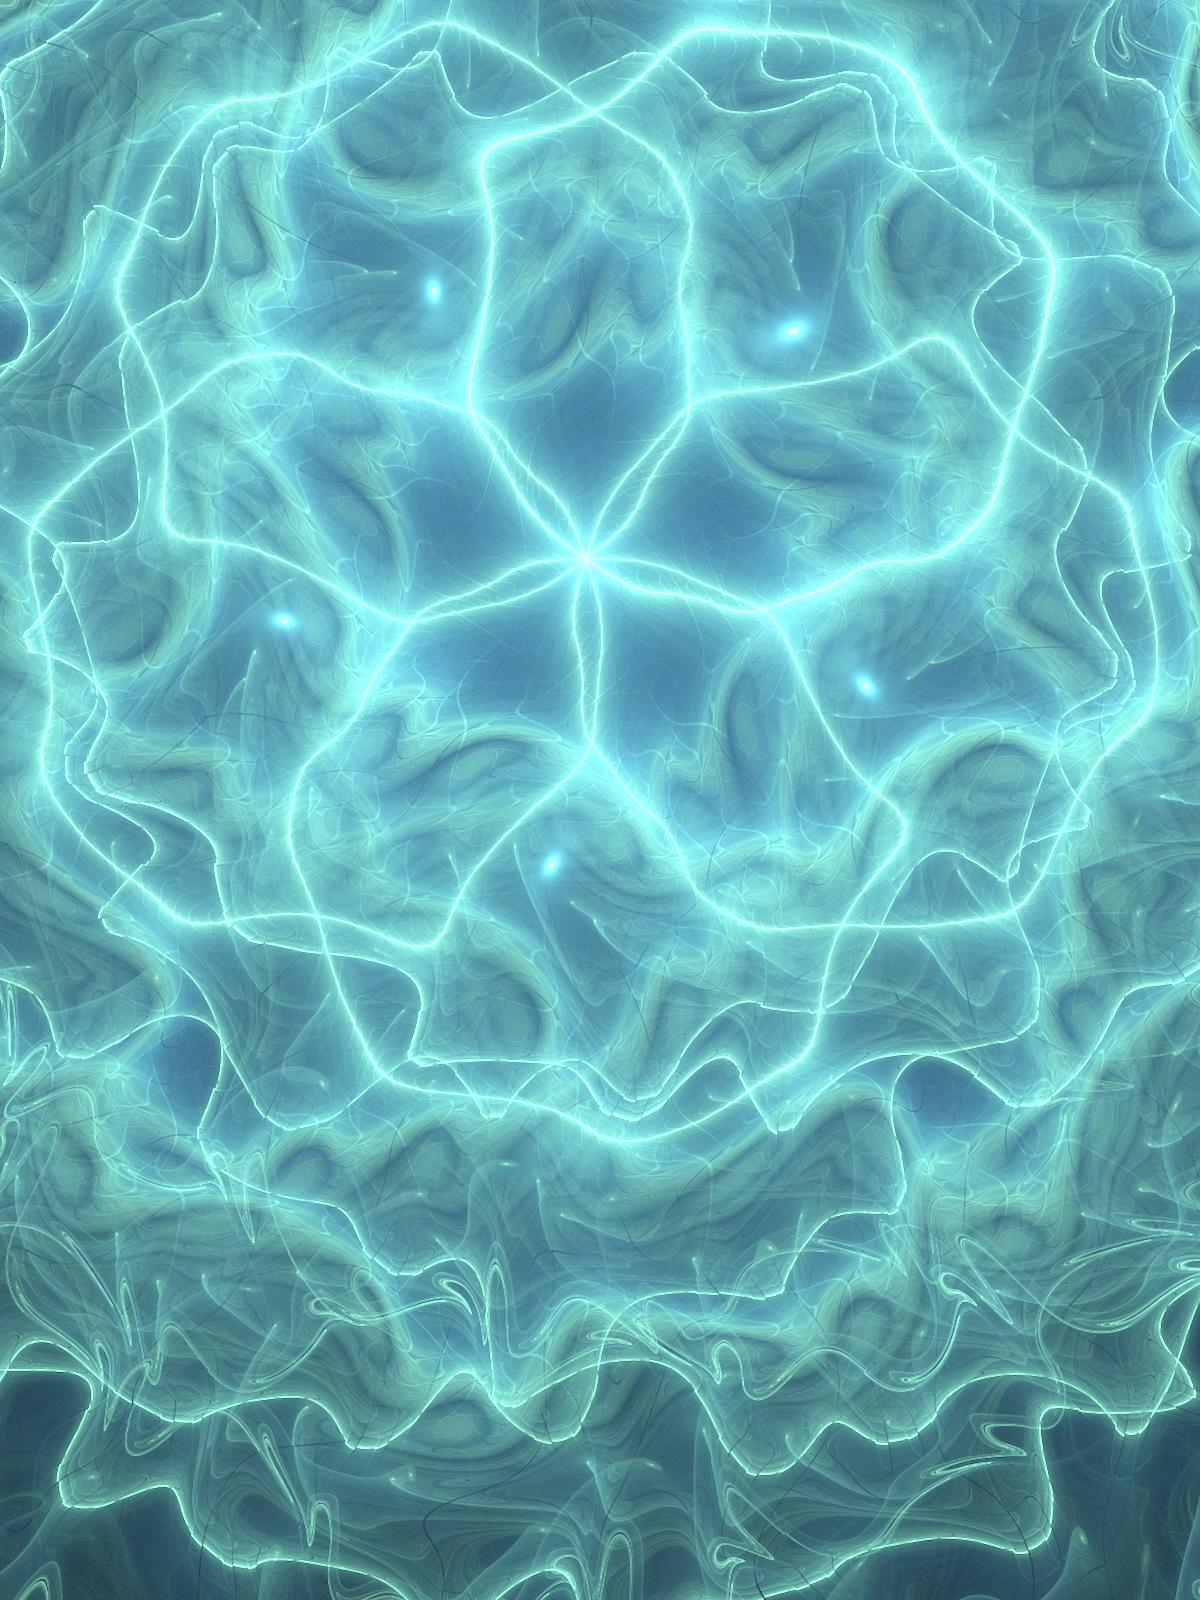
\includegraphics[width=\paperwidth, height=\paperheight]{images/blueback.jpg}};


    

      \begin{scope}[
        shift={(\pagewidth/2, -15cm)},
        draw=white,
        scale=1
      ]
        
        % Define the vector field function
        % Based on Van der Pol's equation with mu=0.08
        \def\vectorfieldx(#1,#2){0.08 * (1 - (#2)^2) * (#1) - (#2)}
        \def\vectorfieldy(#1,#2){(#1)}

        % Draw the vector field
        \foreach \x in {-10,-9.4,...,10}
            \foreach \y in {-6,-5.4,...,6}
            {
                % Calculate the vector at (\x, \y)
                \pgfmathsetmacro\vx{\vectorfieldx(\x,\y)}
                \pgfmathsetmacro\vy{\vectorfieldy(\x,\y)}
                
                % Normalize the vector for consistent arrow lengths
                \pgfmathsetmacro\norm{sqrt(\vx*\vx + \vy*\vy + 0.01)}
                \pgfmathsetmacro\scaleChange{atan(\norm)/100/\norm}
                \pgfmathsetmacro\vx{\vx*\scaleChange}
                \pgfmathsetmacro\vy{\vy*\scaleChange}
                            
                % Draw the vector as an arrow
                \draw[->] (\x,\y) -- ++(\vx,\vy);
            }

        
      \end{scope}



		\fill[path fading=north,covershade] (0,2.2in) rectangle ([yshift=-1.01in, xshift=2pt]current page.north east);
		\fill[covershade] (0,-1in) rectangle ([yshift=-2.05in]current page.north east);
		\fill[path fading=south, covershade] (0,-2in) rectangle ([xshift=1in,yshift=2in]current page.south east);
	\end{scope}


      \begin{scope}[
        shift={(\pagewidth/2, -15cm)},
        draw=white,
        scale=1
      ]
      \draw[very thick, coverblue] plot[smooth] coordinates {
        (-12.0, 7.0)
        (-7.767707632117724, 5.1136037435947825)
        (-6.55029161639424, 3.7063587117266086)
        (-6.291033918196791, 2.431866228538724)
        (-6.411138793864125, 1.1650517227439243)
        (-6.576468000195089, -0.1356950131526572)
        (-6.44221813555265, -1.4455579004483055)
        (-5.698360207820413, -2.6712777707594126)
        (-4.3170951341152985, -3.681408536248483)
        (-2.6524880454540365, -4.37905302197615)
        (-1.1398165469806572, -4.75315228434578)
        (0.01328155024075596, -4.859475753823552)
        (0.821915312513845, -4.770966774085827)
        (1.3846383135974278, -4.547077407312887)
        (1.7961623140784613, -4.227124320660122)
        (2.123678809225348, -3.8341569115250524)
        (2.4094036113245103, -3.3803996968979177)
        (2.6775274852229343, -2.8715397422619997)
        (2.9386885084803342, -2.3098255535481886)
        (3.190838170593432, -1.69663243845697)
        (3.4170363882183348, -1.0351789558166329)
        (3.582009820736538, -0.33385542452399053)
        (3.6319003441010573, 0.38997593972207234)
        (3.5045429976954092, 1.1070520961664807)
        (3.155148685264799, 1.7768762090366046)
        (2.587887900921836, 2.354441418187956)
        (1.8672212901679928, 2.801721875585408)
        (1.092152607672107, 3.0977299491587664)
        (0.3521124991605785, 3.241010555474463)
        (-0.3012250732092604, 3.2444440764401086)
        (-0.8544424867297288, 3.1272473241910546)
        (-1.3177350297141097, 2.9086793500487116)
        (-1.709817254884819, 2.604896520292268)
        (-2.0481012160157013, 2.2283238912763963)
        (-2.3434557798857867, 1.7884967847522988)
        (-2.5972850709562825, 1.2936842300215976)
        (-2.7995318396515483, 0.7529934864707473)
        (-2.9278428747642637, 0.17877669679455344)
        (-2.9498722041815304, -0.4110641575659039)
        (-2.8314891836259553, -0.991783374275332)
        (-2.5513563553185032, -1.532811519414777)
        (-2.1160520694453173, -2.0019036384168625)
        (-1.5647422912668723, -2.3714499982710877)
        (-0.9571888715832826, -2.624054645877739)
        (-0.35223637076719383, -2.7545420554150293)
        (0.208969609093618, -2.767917451822092)
        (0.7074017997129245, -2.6751774466319342)
        (1.1409678733905675, -2.4892999186199094)
        (1.5162256407417851, -2.2226802066727953)
        (1.8412312541603981, -1.8861516827108782)
        (2.1205905684074478, -1.4892157035815488)
        (2.352260492982905, -1.0410753957570995)
        (2.5256766930025374, -0.5521750545501195)
        (2.621620284466748, -0.03595560032841198)
        (2.6151475323385895, 0.489642956954491)
        (2.4828662364408713, 1.0016886486351866)
        (2.213661103089849, 1.4736108153020884)
        (1.8180343344692644, 1.87867104878967)
        (1.3293099813169997, 2.1945867570657827)
        (0.794190797901561, 2.4073061511888207)
        (0.25804987609744895, 2.51222531866222)
        (-0.24631674645531015, 2.512681356829908)
        (-0.7019367638291837, 2.416976971257817)
        (-1.1044256432520505, 2.2354636862561548)
        (-1.4562076752432407, 1.9785897841527467)
        (-1.7610609416378367, 1.6561027105679327)
        (-2.020002614298509, 1.277213574259159)
        (-2.228526532533583, 0.8514469679845532)
        (-2.375195446537731, 0.3899115410835035)
        (-2.4421349478709335, -0.09332365807743277)
        (-2.4084334761470485, -0.5802252701871604)
        (-2.256955233486863, -1.0488170439950872)
        (-1.9829845793569496, -1.4747978246149418)
        (-1.6003924258753368, -1.8347279568172121)
        (-1.1406761821858395, -2.109792485846884)
        (-0.6442804956115891, -2.2885599794563785)
        (-0.14905669061228027, -2.3676084893799945)
        (0.31787754049255496, -2.35009818117491)
        (0.7421113276838633, -2.2433266310881654)
        (1.119138965567409, -2.0564122105339555)
        (1.4496729869999478, -1.7987719532965614)
        (1.7351596765093849, -1.479539797410572)
        (1.9743152064050415, -1.1077853339754915)
        (2.1608397452464505, -0.6933087834541305)
        (2.2825158087168145, -0.2477611748453797)
        (2.3222938452721924, 0.2142407036486867)
        (2.2621209451040585, 0.6744809719789223)
        (2.0894657385199515, 1.1115611348709173)
        (1.8045089626601378, 1.5027415833371311)
        (1.4240855299322206, 1.8269671904607552)
        (0.9791376348682078, 2.06806108994217)
        (0.5063439362135758, 2.216775540958691)
        (0.03852092207133201, 2.2709535708439934)
        (-0.4014265867003714, 2.2340673110395572)
        (-0.8014088727874329, 2.1130654636693826)
        (-1.1573756131866144, 1.9164467311945423)
        (-1.4691961632545818, 1.6530581640768567)
        (-1.7367949045428668, 1.3317096385534777)
        (-1.9571899726047706, 0.961476199282158)
        (-2.1226527145621805, 0.5524838313440343)
        (-2.2203103862699436, 0.116926977800035)
        (-2.2338013602251845, -0.3300282070157654)
        (-2.1474985307327685, -0.7699250501521737)
        (-1.9527863128114766, -1.1817704006299714)
        (-1.6540334248527286, -1.5440681719746923)
        (-1.270731360880768, -1.837720725007975)
        (-0.8336872859941531, -2.0487709476862106)
        (-0.3768634432605625, -2.169889208925666)
        (0.07077143527120053, -2.200151187280596)
        (0.489693712624652, -2.143516599092316)
        (0.8698389827891272, -2.00687369097906)
        (1.2077367718350809, -1.7984036510000627)
        (1.502739299855169, -1.5266371015336484)
        (1.753602991749257, -1.2002432493885946)
        (1.9559428764769988, -0.8284203015062654)
        (2.1008147526865844, -0.421686841288038)
        (2.1748226436409226, 0.007186991769159341)
        (2.162328656981824, 0.4424707012207193)
        (2.0500252847240463, 0.8654457248214958)
        (1.8329280767882254, 1.2554641277632004)
        (1.51919861148228, 1.5921427727068889)
        (1.130697399744855, 1.8581381762698097)
        (0.6981551997160884, 2.041483871058576)
        (0.2532616593047968, 2.1365911862081575)
        (-0.17824373392450243, 2.1437023482517903)
        (-0.579701459542237, 2.067316017148458)
        (-0.9428033294882393, 1.914390887493251)
        (-1.2646214979968802, 1.6929509253499995)
        (-1.5440907544260531, 1.4113626474013903)
        (-1.778947488670822, 1.0782809921866066)
        (-1.9635539369440294, 0.7031235251737777)
        (-2.087896818752325, 0.29686806026276125)
        (-2.138207129951642, -0.12710255097312514)
        (-2.0997089249039522, -0.5524859428559366)
        (-1.9614753387919905, -0.9603155336591611)
        (-1.7220506686066896, -1.3302995021981292)
        (-1.3931134923157114, -1.6431396923995158)
        (-0.998585021637545, -1.8831569144828317)
        (-0.5689931640011031, -2.0402388269692353)
        (-0.13391225551434208, -2.110404276892739)
        (0.28379833982423563, -2.094982022582439)
        (0.6699835181429457, -1.9990034251459907)
        (1.0178468630950517, -1.8295530054695943)
        (1.324897085026137, -1.59458761616797)
        (1.5896448967126573, -1.3024102069389991)
        (1.8088545791135953, -0.9617572738068034)
        (1.9757183707830477, -0.582348425224214)
        (2.0792788944052543, -0.175682874320757)
        (2.1055730240775365, 0.24421200152425207)
        (2.040895821914876, 0.6604698581912402)
        (1.8768516354841762, 1.0539219298799434)
        (1.61548542293274, 1.4046923420456525)
        (1.2717444025090485, 1.694599509255421)
        (0.8712641888363498, 1.9095973507364619)
        (0.44414108668166763, 2.041335554647893)
        (0.017852270600155092, 2.087326642373181)
        (-0.38740254880218733, 2.049897877495028)
        (-0.7596902706986574, 1.934578001084655)
        (-1.0934959761230514, 1.748594590246179)
        (-1.3866259077743752, 1.4998916361508758)
        (-1.6371070224778699, 1.1967822580892171)
        (-1.840730763384624, 0.8481640531758838)
        (-1.9895752022801223, 0.46413286364143536)
        (-2.0718681911500787, 0.05676532753024312)
        (-2.0736665367191685, -0.3592450468258276)
        (-1.9825969322903052, -0.7664950664560172)
        (-1.7929881991203853, -1.145688727688495)
        (-1.510370575292366, -1.4774608039737998)
        (-1.152691840336067, -1.7448119142012528)
        (-0.7469146918320778, -1.9353256694087746)
        (-0.322421488196114, -2.0423399087455065)
        (0.09545032880050824, -2.0647536473458064)
        (0.4889962171687081, -2.005799354548482)
        (0.8482580152449181, -1.8714531921246096)
        (1.1687789621135087, -1.6690841403991947)
        (1.448507639830574, -1.4066598010739297)
    };
      \end{scope}



\newcommand{\titletext}[5]{
	\draw (#1, #2) node[right,opacity=0.55] {	
		\textpdfrender{
		    TextRenderingMode=Fill,
		    LineWidth=1pt,
		    FillColor=#4,
		  }{\fontsize{#5}{100}\fontfamily{phv}\selectfont  \bfseries #3}
	};
	\draw (#1, #2) node[right] {	
		\textpdfrender{
		    TextRenderingMode=Stroke,
		    LineWidth=1pt,
		    StrokeColor=#4,
		  }{\fontsize{#5}{100}\fontfamily{phv}\selectfont  \bfseries #3}
	};
}

\newcommand{\subtitletext}[5]{
	\draw (#1, #2) node[right,opacity=0.55] {	
		\textpdfrender{
		    TextRenderingMode=Fill,
		    LineWidth=1pt,
		    FillColor=#4,
		  }{\fontsize{#5}{100}\fontfamily{phv}\selectfont #3}
	};
	\draw (#1, #2) node[right] {	
		\textpdfrender{
		    TextRenderingMode=Stroke,
		    LineWidth=1pt,
		    StrokeColor=#4,
		  }{\fontsize{#5}{100}\fontfamily{phv}\selectfont #3}
	};
}




  \begin{scope}[yscale=-1, xscale=1, x=2.7pt, y=2.7pt,line join=miter,line cap=butt,line width=1.3pt, yshift=2.3cm, xshift=.7cm,
	  ]

	\coordinate (SUB) at (141, 30);

\begin{bookonly}
	\titletext{6}{23}{Differential Equations}{coverblue}{58}	
\end{bookonly}

\begin{displayonly}
	\titletext{6}{23}{Differential Equations}{coverblue}{50}	
\end{displayonly}


%    \begin{scope}[yscale=-9.7, xscale=9.7, yshift=-.96in]
%	  \fill[coverblue, opacity=.7] \LINEARALGEBRAoutline;
%	  \draw[coverblue, line width=1.3pt] \LINEARALGEBRAoutline;
%    \end{scope}
  \end{scope}
%


  

	\path[white] (SUB) node[anchor=north west] {\Large \bfseries \sffamily \coversubtitle};



\newcommand{\authornames}{\huge \sffamily \bfseries \begin{tabular}{r}Jason Siefken\\Bernardo Galv\~ao-Sousa\end{tabular}}
	\newcommand{\ypadd}{.5em}
	\newcommand{\xpadd}{1em}


\begin{bookonly}
	\draw (0, -24) node[right, xshift=10em] (AUTHOR) {\phantom{\authornames}};	
\end{bookonly}
\begin{displayonly}
	\draw (0, -8.5) node[right, xshift=10em] (AUTHOR) {\phantom{\authornames}};	
\end{displayonly}


	\path let \p1 = (AUTHOR.north) in coordinate (Ab1) at (0,\y1+\ypadd);
	\path let \p1 = (AUTHOR.north east) in coordinate (Ab2) at (\x1+\xpadd,\y1+\ypadd);
	\path let \p1 = (AUTHOR.south east) in coordinate (Ab3) at (\x1+\xpadd,\y1-\ypadd);
	\path let \p1 = (AUTHOR.south) in coordinate (Ab4) at (0,\y1-\ypadd);

	\path[fill=covershade, path fading=west, opacity=.8] (Ab1) -- (Ab2) -- (Ab3) -- (Ab4);
	\draw[covershade!80!black, line width=1.3pt] (Ab1) -- (Ab2) -- (Ab3) -- (Ab4);
\begin{bookonly}
	\draw (0, -24) node[right, xshift=10em, white] (AUTHOR) {\authornames};
\end{bookonly}
\begin{displayonly}
	\draw (0, -8.5) node[right, xshift=10em, white] (AUTHOR) {\authornames};
\end{displayonly}

\end{tikzpicture}


\newpage

\begin{bookonly}
	\clearpage
	\hbox{}
	\newpage
	\begin{center}
	{\color{myorange}\huge\bfseries\sffamily Linear Algebra}\\

\vspace{.2in}
{
\it \copyright\,Jason Siefken, 2016--2022 \\
Creative Commons By-Attribution Share-Alike\, \makebox(30,5){
\includegraphics[height=1.2em]{by-sa.pdf}}
}
\end{center}

\section*{About this Book}

\subsection*{For the student}

This book is your introductory guide to linear algebra. It is divided into
\emph{modules}, and each module is further divided into \emph{exposition},
\emph{practice problems}, and \emph{core exercises}.

The \emph{exposition} is easy to find---it's the text that starts each
module and explains the big ideas of linear algebra.  The \emph{practice
problems} immediately follow the exposition and are there so you can
practice with concepts you've learned.  Following the practice problems
are the \emph{core exercises}. The core exercises build up, through
examples, the concepts discussed in the exposition.

To optimally learn from this text, you should:
\begin{itemize}
	\item Start each module by reading through the \emph{exposition} to get familiar with the main ideas and 
		linear algebra terminology.

	\item Work through the \emph{core exercises} to develop an understanding and intuition behind the main ideas
		and their subtleties.

	\item Re-read the \emph{exposition} and identify which concepts each core exercise connects with.

	\item Work through the \emph{practice problems}. These will serve as a check on whether you've understood
		the main ideas well enough to apply them.
\end{itemize}

{\bf The core exercises.} Most (but not all) core exercises will be
worked through during lecture time, and there is space for you to work
provided after each
of the core exercises. The point of the core exercises is to develop the main ideas of
linear algebra by exploring examples. When working on core exercises, think
``it's the journey that matters not the destination''. The
answers are not the point! If you're struggling, keep with it. The
concepts you struggle with you remember well, and if you look up the
answer, you're likely to forget just a few minutes later. 

{\bf So many definitions.} A big part of linear algebra is learning precise and
technical language\footnote{ Beyond three dimensions, things get very confusing
very quickly.  Having precise definitions allows us to make arguments that
rely on logic instead of intuition; and logic works in all dimensions.}.
There are many terms and definitions you need to learn, and by far the
best way to successfully learn these terms is to understand where they
come from, why they're needed, and practice using them. That is, don't
try to memorize definitions word for word. Instead memorize the idea
and \emph{reconstruct} the definition; go through the core exercises and
identify which definitions appear where; and explain linear algebra to
others using these technical terms.

{\bf Contributing to the book.} Did you find an error? Do you
have a better way to explain a linear algebra concept? Please,
contribute to this book!  This book is open-source, and we welcome
contributions and improvements. To contribute to/fix part of
this book, make a \emph{Pull Request} or open an \emph{Issue} at
\url{https://github.com/siefkenj/IBLLinearAlgebra}. If you contribute,
you'll get your name added to the contributor list.


\subsection*{For the instructor}

This book is designed for a one-semester introductory linear algebra course
course with a focus on geometry (MAT223 at the University of Toronto). 
It has not been designed for an ``intro to proofs''-style course, but could be adapted for one.

Unlike a traditional textbook that is grouped into chapters and sections
by subject, this book is grouped into modules. Each module contains exposition
about a subject, practice problems (for students to work on by themselves), and core exercises
(for students to work on with your guidance). Modules group related concepts, but the 
modules have been designed to facilitate learning linear algebra rather than to serve
as a reference. For example, information about change-of-basis is spread across several non-consecutive
modules; each time change-of-basis is readdressed, more detail is added.

{\bf Using the book.} This book has been designed for use in large 
active-learning classrooms driven by a \emph{think, pair-share}/small-group-discussion format.
Specifically, the \emph{core exercises} (these are the problems which aren't labeled ``Practice Problems''
and for which space is provided to write answers) are designed for use during class time.

A typical class day looks like:
\begin{enumerate}
	\item {\bf Student pre-reading.} Before class, students will read through the relevant module.

	\item {\bf Introduction by instructor.} This may involve giving a definition,
		a broader context for the day's topics, or answering questions.

	\item {\bf Students work on problems.} Students work individually or in pairs/small groups
		on the prescribed core exercise. During this time the instructor moves
		around the room addressing questions that students may have and giving
		one-on-one coaching.

	\item {\bf Instructor intervention.} When most students have successfully solved
		the problem, the instructor refocuses the class by providing an
		explanation or soliciting explanations from students.
		This is also time for the instructor to ensure that everyone has
		understood the main point of the exercise (since it is sometimes
		easy to miss the point!).

		If students are having trouble, the instructor can give hints
		and additional guidance to ensure students' struggle is productive.

	\item {\bf Repeat step 3.}
\end{enumerate}

Using this format, students are thinking (and happily so) most of the class. Further,
after struggling with a question, students are especially primed to hear the insights of the instructor.

{\bf Conceptual lean.}
The \emph{core exercises} are geared towards concepts instead of computation, though some core exercises
focus on simple computation. They also have a geometric lean. Vectors are initially
introduced with familiar coordinate notation, but eventually, coordinates are understood to be
\emph{representations} of vectors rather than ``true'' geometric vectors, and objects like the
determinant are defined via oriented volumes rather than formulas involving matrix entries.

Specifically lacking are exercises focusing on the mechanical skills of row reduction and
computing matrix inverses. Students must practice these skills, but they require little instructor
intervention and so can be learned outside of lecture (which is why core exercises don't focus on
these skills).

{\bf How to prepare.}
Running an active-learning classroom is less scripted than lecturing.
The largest
challenges are: (i) understanding where students are at, (ii) figuring out what to do given the current
understanding of the students, and (iii) timing.

To prepare for a class day, you should:
\begin{enumerate}
	\item {\bf Strategize about learning objectives.} Figure out what the point of the day's lesson is
		and brain storm some examples that would illustrate that point.
	\item {\bf Work through the core exercises.} 
	%	By working through the exercises yourself, you
	%	will be ready to build off student reasoning, and better able to direct a class towards
	%	the important ideas\footnote{ The content of linear algebra is fairly non-linear. One of the hardest parts
	%	of teaching linear algebra is coming up with an explanation that only depends on ideas that have already been taught.}.
	\item {\bf Reflect.} Reflect on how each core exercise addresses the day's goals. Compare with the examples you
		brainstormed and prepare follow-up questions that you can use in class to test for understanding.
	\item {\bf Schedule.} Write timestamps next to each core exercise indicating at what minute you hope
		to start each exercise. Give more time for the exercises that you judge as foundational, and be prepared
		to triage. It's appropriate to leave exercises or parts of exercises for homework, but change the order
		of exercises at your peril---they really do build on each other.
\end{enumerate}

A typical
50 minute class is enough to get through 2--3 core exercises (depending on the difficulty), and class observations
show that class time is split 50/50 between students working and instructor explanations.

\subsection*{License}
 Unless otherwise mentioned, pages of this document are licensed under
the Creative Commons By-Attribution Share-Alike License. That means, you are free
to use, copy, and modify this document provided that you provide attribution to the
previous copyright holders and you release your derivative work under the same license.
Full text of the license is at \url{http://creativecommons.org/licenses/by-sa/4.0/}

If you modify this document, you may add your name to the copyright list. Also,
if you think your contributions would be helpful to others, consider making a
pull request, or opening an \emph{issue} at \url{https://github.com/siefkenj/IBLLinearAlgebra}

{\bf Incorporated content.}
Content from other sources is reproduced here with permission and retains the
Author's copyright. Please see the footnote of each page to verify the
copyright.

Included in this text are tasks created by the Inquiry-Oriented Linear Algebra (IOLA) project. Details
about these tasks can be found on their website \url{http://iola.math.vt.edu/}. Also included are some
practice problems from Beezer's \emph{A First Course in Linear Algebra} (marked with the symbol \beezer next to the
problem), and from Hefferon's \emph{Linear Algebra} (marked with the symbol \hefferon next to the problem).

{\bf Contributing.} You can report errors in the book or contribute to the book by filing an \emph{Issue} or
a \emph{Pull Request} on the book's GitHub page: \url{https://github.com/siefkenj/IBLLinearAlgebra/}


	\section*{Contributors}
	% sorting code from
% http://tex.stackexchange.com/questions/121489/alphabetically-display-the-items-in-itemize
\newcommand{\sortitem}[2][\relax]{%
  \DTLnewrow{list}% Create a new entry
  \ifx#1\relax
    \DTLnewdbentry{list}{sortlabel}{#2}% Add entry sortlabel (no optional argument)
  \else
    \DTLnewdbentry{list}{sortlabel}{#1}% Add entry sortlabel (optional argument)
  \fi%
  \DTLnewdbentry{list}{description}{#2}% Add entry description
}
\newenvironment{sortedlist}{%
  \DTLifdbexists{list}{\DTLcleardb{list}}{\DTLnewdb{list}}% Create new/discard old list
}{%
  \DTLsort{sortlabel}{list}% Sort list
  \begin{itemize*}[label={\color{mypink}$\circ$}]%
    \DTLforeach*{list}{\theDesc=description}{%
      \item \theDesc}% Print each item
  \end{itemize*}%
}

This book is a collaborative effort.  The following people have contributed
to its creation:
\begin{quote}
\begin{sortedlist}
	\sortitem[Wang]{Tianhao (Patrick) Wang}
	\sortitem[Khan]{Sameul Khan}
	\sortitem[King]{Avery King}
	\sortitem[Frohlich]{Jesse Frohlich}
	\sortitem[Wolske]{Zack Wolske}
	\sortitem[Le]{Dan Le}
	\sortitem[Qiu]{Ruo Ning (Nancy) Qiu}
    \sortitem[Li]{Xintong (Alucart) Li}
    \sortitem[Chen]{Shukui Chen}
    \sortitem[Kim]{Julia Kim}
    \sortitem[El-Sheikha]{Hassan El-Sheikha}
    \sortitem[Wang]{Robert Wang}
\end{sortedlist}
{\color{mypink}$\circ$}
\end{quote}

	\section*{Dedication}
	\begin{center}
		This book is dedicated to
		\href{https://www.gazettetimes.com/news/local/obituaries/dr-robert-main-burton/article_9c087f07-c005-515a-bb3f-2c9c6a6b7332.html}{\color{blue}Dr.~Bob Burton}---friend and mentor.

		\emph{\large ``Sometimes you have to walk the mystical path with practical feet.''}
	\end{center}
	\newpage
	\mbox{}
	{
		\pagestyle{empty}
		\setcounter{tocdepth}{1}
		\tableofcontents
		\thispagestyle{empty}
	}
	\newpage
	\mbox{}
	\newpage
\end{bookonly}

\setcounter{page}{1}
\pagestyle{siefken}


\addcontentsline{toc}{chapter}{Lessons}

\begin{module}\label{module1}
	\Title{Modeling}

	In this module you will learn
	\begin{itemize}
		\item ??
	\end{itemize}

	\Heading{Modeling}

Suppose you are observing some \emph{green} ants walking on the sidewalk.
In the first minute you record 10 ants. In the second minute you
record 20. In the third minute, you record 40 ants. This continues until
there are too many ants for you to count.

\begin{center}
	\begin{tabular}{c|c}
		Minute & \#Green Ants\\
		\hline
		1 & 10\\
		2 & 20\\
		3 & 40\\
		4 & 80\\
		$\vdots$ & $\vdots$
	\end{tabular}
\end{center}

Since you lost count of the ants, you decide to use mathematics to try and figure out
how many ants walked by on minutes $5$, $6$, \ldots. You notice the pattern that
\[
	\text{Green ants per minute $n$} = 2^{n-1}\cdot 10.
\]
Stupendous! Mathematics now predicts there were $160$ ants during minute $5$. But something
else catches your eye. Across the sidewalk are \emph{brown} ants. You count these
ants every minute.

\begin{center}
	\begin{tabular}{c|c}
		Minute & \#Brown Ants\\
		\hline
		1 & 3\\
		2 & 6\\
		3 & 12\\
		4 & 24\\
		$\vdots$ & $\vdots$
	\end{tabular}
\end{center}

The pattern is slightly different. This time, 
\[
	\text{Green ants per minute $n$} = 2^{n-1}\cdot 3.
\]

Your friend, who was watching you the whole time, looks confused. ``Why come up with two complicated equations
when you can describe both types of ant at once?'' they declare.

\begin{center}
	\begin{tabular}{c}
		$\text{\#Ants at minute $n$}\ =\ 2\cdot(\text{\#Ants at minute $n-1$})$\\
		$\text{\#Green ants at minute 1}=10$\\
		$\text{\#Brown ants at minute 1}=3$\\
	\end{tabular}
\end{center}

Your friend has a point. Their model is elegant, but \emph{your} model can predict how many ants pass by at minute $3.222$!
Though, your friend would probably complain that $46.654$ is not a number of ants\ldots.

\medskip

You and your friend have just come up with two different \emph{mathematical models} for the number of ants
that walk across the sidewalk. They happen to make similar predictions for each minute and each have their
strengths and weakenesses. In this course, we will be focused on a particular type of mathematical model---one
that uses \emph{differential equations} at its core.

\Heading{Types of Models}

\begin{definition}[Mathematical Model]
A \emph{mathematical model}\index{model} is a description of the world
	\begin{enumerate}
		\item created in the service of answering a question, and
		\item where the complexity of the world has been abstracted away to numbers, quantities, and their relationships\footnote{ Other
mathematical objects are also allowed.}.
	\end{enumerate}
\end{definition}

In the previous situation, the \emph{question} you were trying to answer was ``how many ants are there at a given minute?''.
We sidestepped difficult issues like, ``Is an ant that is missing three legs still an ant?'' by using the common-sense
convention that ``the number of ants is a whole number and one colored blob that moves under its own power corresponds to one ant''; thus,
we could use single numbers to represent our quantity of interest (the ants).

You and your friend already came up with two types of models.
\begin{itemize}
	\item An \textbf{analytic} model based on known functions.
	\item A \textbf{recursive} model where subsequent terms are based on previous terms and initial conditions.
\end{itemize}

If we define $A(n)$ to be the number of ants corssing the sidewalk at minute $n$, the \emph{analytic} model presented for green ants is
\[
	A(n)=2^{n-1}\cdot 10
\]
and the \emph{recursive} model presented is
\begin{align*}
	A(1) &= 10\\
	A(n) &= 2\cdot A(n-1).
\end{align*}

Each type of model has pros and cons. For example, the analytic model allows you to calculate the number of ants at any minute
with few button presses on a calculator, whereas the recursive model is more difficult to calculate but
makes it clear that the number of ants is doubling every minute.

Often times recursive models are easier to write down than analytic models\footnote{ In fact, in many real-world situations, an analytic model
doesn't exist}, but they maybe harder to analyze. A third type of model has similarities to both analytic and recursive models, and
brings the power of calculus to modeling.

\begin{itemize}
	\item A \textbf{differential-equations} model is a model based on a relationship between a function's derivative(s), its values, and initial conditions.
\end{itemize}

\emph{Differential-equations} models are useful because derivatives correspond to rates of change---and things in the world are always changing.
Let's try to come up with a differential equations model for the ants.

We'd like an equation relating $A(n)$, the number of ants at minute $n$, to $A'(n)$, the \emph{instantaneous rate of change} of the number of ants at minute $n$.
Making a table, we see

\begin{center}
	\begin{tabular}{c|c|c}
		Minute & \#Brown Ants & Change (from prev. minute)\\
		\hline
		1 & 3 & ?\\
		2 & 6 & 3\\
		3 & 12 & 6\\
		4 & 24 & 12\\
	\end{tabular}
\end{center}

or

\begin{center}
	\begin{tabular}{c|c|c}
		Minute & \#Brown Ants & Change (from next minute)\\
		\hline
		1 & 3 & 3\\
		2 & 6 & 6\\
		3 & 12 & 12\\
		4 & 24 & ?\\
	\end{tabular}
\end{center}

depending on whether we record the change from the previous minute or up to the subsequent minute. Neither table gives the \emph{instantaneous} rate of
change, but in both tables, the change is proportional to the number of ants. So, we can set up a model
\[
	A'(n) = kA(n)
\]
where $k$ is a constant of proportionality that we will try to determine later. We've just written down a \emph{differential equation} with an undetermined parameter, $k$.

\begin{definition}[Differential Equation]
	A \emph{differential equation}\index{differential equation} is an equation relating a function to one or more of its derivatives.
\end{definition}

We'd like to figure out what $k$ is. One way to do so is to solve the differential equation and find the values of $k$ so that our model
correctly predicts the data. This is called \emph{fitting} the model to data.

\begin{definition}[Fitting a Model]
	Given a model $M$ with parameters $k_1$, $k_2$, $\ldots$ and data $D$, \emph{fitting the model $M$ to the data $D$}
	is the process of finding values for the parameters $k_1$, $k_2$, $\ldots$ so that $M$ most accurately predicts the data $D$.
\end{definition}

Note that, in general, fitting a model to data doesn't necessarily produce \emph{unique} values for the unknown parameters, and a fitted model
(especially when the data comes from real-world observations) usually doesn't reproduce the data exactly. However, in the case of these ants, we
just might get lucky.

\Heading{Solving Differential Equations}

In general, \emph{there is no algorithm for solving differential equations}. Fortunately, it is easy to check whether any particular
function is a solution to a differential equation, since there \emph{is} an algorithm to differentiate functions\footnote{ More specifically, there is an algorithm
to differentiate the \emph{elementary} functions, those functions formed by compositions, sums, products, and quotients of polynomials, trig, exponentials, and logs.}.
Because of this, \emph{guess and check} will be our primary method for solving differential equations.

\begin{example}
Use educated guessing to solve $A'(n)=kA(n)$.

Since $A'\approx A$, we might start with a function that is equal to its own derivative. There is a famous one: $e^n$. Testing, we see
\[
	\frac{\d}{\d n}e^n=e^n=ke^n
\]
if $k=1$, but it doesn't work for other $k$'s. Trying $e^{kn}$ instead yields
\[
	\frac{\d}{\d n}e^{kn}=ke^{kn}
\]
which holds for all $k$. Thus $A(n)=e^{kn}$ is \emph{a} solution to $A'(n)=kA(n)$. However, there are other solutions, because
\[
	\frac{\d}{\d n}Ce^{kn}=C\left(ke^{kn}\right)=k\left(Ce^{kn}\right),
\]
and so for every $C$, the function $A(n)=Ce^{kn}$ is a solution to $A'(n)=kA(n)$.
\end{example}

By guessing-and-checking, we have found an infinite number of solutions to $A'(n)=kA(n)$.  It's now time to fit our
model to the data.

\begin{example}
	Find values of $C$ and $k$ so that $A(n)=Ce^{kn}$ best models brown ants.

	Taking two rows from our brown ants table, we see
	\begin{align*}
		A(1) &= Ce^{k} = 3\\
		A(2) & = Ce^{2k}=6.
	\end{align*}

	Since $e^k$ can never be zero, from the first equation we get $C=3/e^k$. Combining with the second equation we find
	\[
		Ce^{2k}=\frac{3}{e^k}e^{2k}=3e^k=6
	\]
	and so $e^k=2$. In other words $k=\ln 2$. Plugging this back in, we find $C=3/2$. Thus our fitted model is
	\[
		A(n)=\tfrac{3}{2}e^{n\ln 2}.
	\]
\end{example}

Upon inspection, we can see that $\tfrac{3}{2}e^{n\ln 2} = 3\cdot 2^{n-1}$, which is the analytic model
that was first guessed for brown ants.



%One of the beauties of the guess-and-check method is that it \emph{cannot} produce an incorrect answer,
%since you're always checking (though it may fail to produce answers, any answer that it \emph{does} produce
%will be correct). Thus, even if you did some mathematically-dubious steps to produce a guess, if it passes the checks,
%the final answer is valid.
%
%\begin{example}
%Use Leibniz notation, integral calculus, and guess-and-check to come up with solutions to $A'(n)=kA(n)$.
%
%In Leibniz notation, $A'(n)$ is written as $\displaystyle\frac{\d A}{\d n}$, and we may suppress the function variable and write $A$ in place of $A(n)$. Thus, our equation becomes
%\[
%	\frac{\d A}{\d n}=kA.
%\]
%Treating $\d A/\d n$ as an actual ratio, we can bring all $A$'s to the left and $n$'s to the right, giving
%\[
%	\frac{1}{A}\d A = k\d n.
%\]
%Integrating both sides gives
%\[
%	\int \frac{1}{A}\d A = \ln A + C_1 \qquad =\qquad  \int k\d n = kn + C_2,
%\]
%and so
%\[
%	\ln A + C_1 = kn + C_2 \qquad \iff \qquad \ln A = kn + (C_2-C_1) = kn + C_3.
%\]
%Solving for $A$ by exponentiating both sides gives
%\[
%	A = e^{\ln A} = e^{kn + C_3} = C_4 e^{kn}.
%\]
%Much of what we've done in the preceding calculation \emph{was not rigorous mathematics}, but that's okay, because
%it leads us to the guess: $A(n)=Ce^{kn}$. Finally, we can test our guess and verify
%\[
%	\frac{\d}{\d n}Ce^{kn}=C\left(ke^{kn}\right)=k\left(Ce^{kn}\right),
%\]
%and so $A(n)=Ce^{kn}$ is a solution for every $C$.\footnote{ Notice that in our ``guess work'', $C_4$ was actually restricted to be a positive
%number, but our solution works with $C$ being positive or negative.}
%
%\end{example}




	%\begin{exercises}
		% Topics:
		% Sets, set builder notation, set operations,
		% vectors \& scalars, vector notation, vectors \& points, vector arithmetic,
		% coordinates \& the standard basis, higher dimensions,
	\begin{problist}
		% Computation (4 questions)
		\prob
		\begin{enumerate}
			\item
			Write the following vectors as column vectors.
			\begin{enumerate}
				\item $4\xhat -3\zhat +2\yhat -2\xhat\in\R^3$.
				\item $\yhat +\xhat -5\yhat \in\R^2$.
			\end{enumerate}
			\item
			Write the following vectors as linear combinations of
			$\xhat$, $\yhat$, and $\zhat$.
			\begin{enumerate}
				\item $\mat{1\\-2\\3}$.
				\item $\mat{-2\\5\\4} + \mat{1\\-2\\ -5} + \mat{1\\0\\1}$.
			\end{enumerate}
		\end{enumerate}
		% Q1 Solution
		\begin{solution}
			\begin{enumerate}
				\item
				\begin{enumerate}
					\item $\mat{2\\2\\-3}$
					\item $\mat{1\\-4}$
				\end{enumerate}
				\item
				\begin{enumerate}
					\item $\xhat - 2\yhat + 3\zhat$
					\item $3\yhat$
				\end{enumerate}
			\end{enumerate}
		\end{solution}

		\prob
		Compute
		\[
			3\mat{2\\-1\\1\\1\\0}+
			(-2)\mat{1\\2\\-7\\3\\0}+
			\mat{-3\\3\\9\\2\\2}
		\]
		% Q2 Solutions
		\begin{solution}
		    $\mat{1\\-4\\26\\-1\\2}$
		\end{solution}

		\prob[\hefferon[2.21,2.22]]
		Decide if the vector is in the set. If it is, what value of the
		parameters produce that vector?
		\begin{enumerate}
			\item $\mat{5\\-5}$ and the set
			\[
				\Set*{\vec{v}\in\R^2 \given \vec{v}=k\mat{1\\-1} \text{ for some } k\in\R}
			\]
			\item $\mat{-1\\2\\1}$ and the set
			\[
				\Set*{\vec{v}\in\R^3 \given
				\vec{v}=i\mat{-2\\1\\0}+j\mat{3\\0\\1} \text{ for some } i,j\in\R}
			\]
			\item $\mat{3\\-1}$ and the set
			\[
				\Set*{\vec{v}\in\R^2 \given \vec{v}=k\mat{-6\\2} \text{ for some } k\in\R}
			\]
			\item $\mat{5\\4}$ and the set
			\[
				\Set*{\vec{v}\in\R^2 \given \vec{v}=j\mat{5\\-4} \text{ for some } j\in\R}
			\]
			\item $\mat{2\\1\\-1}$ and the set
			\[
				\Set*{\vec{v}\in\R^3 \given \vec{v}=r\mat{1\\-1\\3}+\mat{0\\3\\-7} \text{ for some } r\in\R}
			\]
			\item $\mat{1\\0\\1}$ and the set
			\[
				\Set*{\vec{v}\in\R^3 \given \vec{v}=j\mat{2\\0\\1}+k\mat{-3\\-1\\1} \text{ for some } j,k\in\R}
			\]
		\end{enumerate}
		% Q3 solution
		\begin{solution}
			\begin{enumerate}
		        \item Yes, take $k=5$.
		        \item Yes, take $i=2,j=1$.
		        \item Yes, take $k=-\frac{1}{2}$.
		        \item No.
		        \item Yes, take $r=2$.
		        \item No.
		    \end{enumerate}
		\end{solution}

		% Conceptual (3 questions)
		\prob
		% Purpose: get students to understand (the beginnings of) scale-invariance
		% of bases, as well as carefully reading mathematical expressions.
		Draw the following subsets of $\R^2$ and then determine which are equal or subsets of each other.
		\begin{enumerate}
			\item $A=\Set*{\vec v\in\R^2\given \vec v=n\mat{2\\1}\text{ for some integer }n\in\Z}$
			\item $B=\Set*{\vec v\in\R^2\given \vec v=t\mat{4\\2}\text{ for some }t\in\R}$
			\item $C=\Set*{\vec v\in\R^2\given \vec v=n\mat{4\\2}\text{ for some integer }n\in\Z}$
			\item $D=\Set*{\vec v\in\R^2\given \vec v=t\mat{2\\1}\text{ for some }t\in\R}$
		\end{enumerate}
		\begin{solution}
			\begin{enumerate}
				\item 
				\begin{tikzpicture}[baseline = (current bounding box.north)]
					\begin{axis}[
						anchor=origin,
						disabledatascaling,
						xmin=-4,xmax=4,
						ymin=-4,ymax=4,
						xtick={-4,-2,0,2,4},
						ytick={-4,-2,0,2,4},
						x=0.5cm,y=0.5cm,
						grid=both,
						grid style={line width=.1pt, draw=gray!10},
						axis lines=middle,
						minor tick num=0,
						enlargelimits={abs=1.0},
						axis line style={latex-latex},
						ticklabel style={font=\tiny,fill=white},
						xlabel style={at={(ticklabel* cs:1)},anchor=north west},
						ylabel style={at={(ticklabel* cs:1)},anchor=south west}
					]
					\end{axis}
					\foreach \n in {-2,...,2} {
						\fill [mypink] (\n,\n/2) circle[radius=2pt];
					}
				\end{tikzpicture}
				\item 
				\begin{tikzpicture}[baseline = (current bounding box.north)]
					\begin{axis}[
						anchor=origin,
						disabledatascaling,
						xmin=-4,xmax=4,
						ymin=-4,ymax=4,
						xtick={-4,-2,0,2,4},
						ytick={-4,-2,0,2,4},
						x=0.5cm,y=0.5cm,
						grid=both,
						grid style={line width=.1pt, draw=gray!10},
						axis lines=middle,
						minor tick num=0,
						enlargelimits={abs=1.0},
						axis line style={latex-latex},
						ticklabel style={font=\tiny,fill=white},
						xlabel style={at={(ticklabel* cs:1)},anchor=north west},
						ylabel style={at={(ticklabel* cs:1)},anchor=south west}
					]
						\draw [mygreen, thick] (-5,-2.5) -- (5,2.5);
					\end{axis}
				\end{tikzpicture}
				\item 
				\begin{tikzpicture}[baseline = (current bounding box.north)]
					\begin{axis}[
						anchor=origin,
						disabledatascaling,
						xmin=-4,xmax=4,
						ymin=-4,ymax=4,
						xtick={-4,-2,0,2,4},
						ytick={-4,-2,0,2,4},
						x=0.5cm,y=0.5cm,
						grid=both,
						grid style={line width=.1pt, draw=gray!10},
						axis lines=middle,
						minor tick num=0,
						enlargelimits={abs=1.0},
						axis line style={latex-latex},
						ticklabel style={font=\tiny,fill=white},
						xlabel style={at={(ticklabel* cs:1)},anchor=north west},
						ylabel style={at={(ticklabel* cs:1)},anchor=south west}
					]
					\end{axis}
					\foreach \n in {-1,...,1} {
						\fill [mypink] (\n*2,\n) circle[radius=2pt];
					}
				\end{tikzpicture}
				\item 
				The set $D$ and $B$ are equal.
			\end{enumerate}
			We have $C\subseteq A$, $C\subseteq B$, $C\subseteq D$,  $A\subseteq B$, $A\subseteq D$, and $B=D$.
		\end{solution}

		\prob
		Let $\vec a=\mat{1\\2}$, $\vec b=\mat{2\\4}$, $\vec c=\xhat+3\yhat$, and $\vec d=\vec a+\vec c$.
		\begin{enumerate}
			\item Is $\xhat$ a linear combination of $\vec a$ and $\vec b$?
			\item Is $\vec d$ a linear combination of $\vec a$ and $\vec b$?
			\item Is $\vec p=\mat{1\\1}$ a linear combination of $\vec a$ and $\vec c$?
			\item Is $\vec q=\mat{-3\\3}$ a linear combination of $\vec a$, $\vec b$, $\vec c$, and $\vec d$?
		\end{enumerate}
		% Q5 Solutions
		\begin{solution}
            \begin{enumerate}
    		    \item No.
    		    \item No.
    		    \item Yes.
    		    \item Yes.
		    \end{enumerate}
		\end{solution}
		
		\prob
		Use set-builder notation to describe the following sets.
		\begin{enumerate}
			\item The set of vectors in $\R^{2}$ whose coordinates are rational numbers.

			\item The set of vectors in $\R^{2}$ whose coordinates are irrational
				numbers.

			\item Let $P(\vec x) = -\vec x$. The set $\Set*{P(\vec e_{1}), P(\vec e_{2})}$.
		\end{enumerate}
		\begin{solution}
			\begin{enumerate}
				\item $\Set*{\vec{v}\in\R^2 \given \vec{v}=\mat{\alpha\\\beta} \text{ for some } \alpha,\beta\in\Q}$
				\item $\Set*{\vec{v}\in\R^2 \given \vec{v}=\mat{\alpha\\\beta} \text{ for some } \alpha,\beta\in\R\setminus\Q}$
				\item $\Set*{\vec{v}\in\R^2 \given \vec{v}=-\vec{e}_1 \text{ or } \vec{v}=-\vec{e}_2}$
			\end{enumerate}
		\end{solution}

		% Challenge (3 questions)
		\prob % Propose: get students to understand quantifiers and set operations
		% practice providing justification to their intuitive guesses
		Which of the following statements are true about the set listed below? Justify your
		answers.
		\begin{enumerate}
			\item $\mathcal{Y}$, the $y$-axis in $\R^{3}$.
				\begin{enumerate}
					\item $\mathcal{Y}$ is a finite set.

					\item Let
						\[
							\mathcal{A} = \Set*{\vec a \in \R^3 \given \vec a = \beta \vec v
										  \text{ for some } \vec v \in \mathcal{Y}, \beta \in \R},
						\]
						then $\mathcal{A} \subseteq \mathcal{Y}$.

					\item For all vectors $\vec v \in \mathcal{Y}$, we have $\vec v \neq
						\vec 0$.

					\item For some vectors $\vec v \in \mathcal{Y}$, we have $\vec v
						\neq \vec 0$.

					\item For all vectors $\vec v \in \mathcal{Y}$, there exists a vector
						$\vec x \in \mathcal{Y}$ such that $\vec x + \vec v = \vec e_{2}$.

					\item There exists a vector $\vec x \in \mathcal{Y}$ such that for
						all vectors $\vec v \in \mathcal{Y}$, we have $\vec x + \vec v =
						\vec e_{2}$.
				\end{enumerate}

			\item $\mathcal{S}$, the set of vectors in $\R^{3}$ whose coordinates are $\pm3$.
				\begin{enumerate}
					\item $\mathcal{S}$ is a finite set.

					\item Let
					\[
						\mathcal{A} = \Set*{\vec a \in \R^3 \given \vec a = \beta \vec v
									  \text{ for some } \vec v \in \mathcal{S}, \beta \in \R },
					\]
					then $\mathcal{A} \subseteq \mathcal{S}$.

					\item For all vectors $\vec v \in \mathcal{S}$, we have $\vec v \neq
						\vec 0$.

					\item For some vectors $\vec v \in \mathcal{S}$, we have $\vec v
						\neq \vec 0$.

					\item For all vectors $\vec v \in \mathcal{S}$, there exists a vector
						$\vec x \in \mathcal{S}$ such that $\vec x + \vec v = \vec 0$.

					\item There exists a vector $\vec x \in \mathcal{S}$ such that for
						all vectors $\vec v \in \mathcal{S}$, we have $\vec x + \vec v =
						\vec 0$.
				\end{enumerate}
		\end{enumerate}
		\begin{solution}
			\begin{enumerate}
				\item 
				\begin{enumerate}
					\item False.
					\item True.
					\item False.
					\item True.
					\item True.
					\item False.
				\end{enumerate}
				\item 
				\begin{enumerate}
					\item True.
					\item False.
					\item True.
					\item True.
					\item True.
					\item False.
				\end{enumerate}
			\end{enumerate}
		\end{solution}

		\prob % Propose: Give students some practices on proving general statements about sets
		For each of the following statements, determine whether it is correct or not. If
		it is, prove it. Otherwise, give a counterexample.
		\begin{enumerate}
			\item If $A \subseteq B$, then $A \cap B = A$.

			\item If $B \subseteq A$, then $A \cap B = A$.

			\item If $A \subseteq B$, then $A \cap B \neq B$.

			\item If $B \subseteq A$, then $A \cap B \neq B$.

			\item If $C \subseteq A \cap B$, then $C \subseteq A$.

			\item If $C \subseteq A \cup B$, then $C \subseteq A$.

			\item If $C \subseteq A \cup B$ and $C \subseteq B$, then $A \cap B
				\subseteq C$.
		\end{enumerate}
		\begin{solution}
			\begin{enumerate}
				\item Correct.
				\item Incorrect.
				\item Incorrect.
				\item Incorrect.
				\item Correct.
				\item Incorrect.
				\item Incorrect.
			\end{enumerate}
		\end{solution}
	\end{problist}
\end{exercises}

\end{module}

%
% Hours 1-6
%

\begin{slide}
	\question
	You are observing starfish that made their way to a previously uninhabited tide-pool.
	You'd like to predict the year-on-year population of these starfish.

	You start with a simple assumption
	\[
		\# \text{new children per year}\ \sim\ \text{size of current population}
	\]
	\begin{parts}
		\item Come up with a mathematical model for the number of star fish in a given year.
		Your model should
		\begin{itemize}
			\item Define any notation (variables and parameters) you use
			\item Include at least one formula/equation
			\item Explain how your formula/equation relates to the starting assumption
		\end{itemize}
	\end{parts}
\end{slide}

\begin{slide}
	\question
		Let

		\begin{tabular}{rl}
			(Birth Rate) & $K=1.1$ children per starfish per year \\
			(Initial Pop.) & $P_0=10$ star fish
		\end{tabular}

		and define the model \textbf{M$_1$} to be the model for starfish population with
		these parameters.
	\begin{parts}
		\item Simulate the total number of starfish per year using Excel.
	\end{parts}
\end{slide}

\begin{slide}
	\question
	Recall the model \textbf{M$_1$} (from the previous question). 

	Define the model \textbf{M$_1^*$} to be
	\[
		P(t) = P_0 e^{0.742 t}
	\]
	\begin{parts}
		\item Are \textbf{M$_1$} and \textbf{M$_1^*$} different models or the same?
		\item Which of \textbf{M$_1$} or \textbf{M$_1^*$} is better?
		\item List an advantage and a disadvantage for each of \textbf{M$_1$} and \textbf{M$_1^*$}.
	\end{parts}
\end{slide}

\begin{slide}
	\question
	In the model \textbf{M$_1$}, we assumed the starfish had $K$ children at one point during the year.

	\begin{parts}
		\item Create a model \textbf{M$_n$} where the starfish are assumed to have $K/n$ children $n$ times per year (at regular intervals).
		\item Simulate the models \textbf{M$_1$}, \textbf{M$_2$}, \textbf{M$_3$} in Excel. Which grows fastest?
		\item What happens to \textbf{M$_n$} as $n\to\infty$?
	\end{parts}

\end{slide}

\begin{slide}
	\question
	Exploring \textbf{M$_n$}

	We can rewrite the assumptions of \textbf{M$_n$} as follows:
	\begin{itemize}
		\item At time $t$ there are $P_n(t)$ starfish.
		\item $P_n(0)=10$
		\item During the time interval $(t, t+1/n)$ there will be (on average) $K/n$ new children per starfish.
	\end{itemize}

	\begin{parts}
		\item Write an expression for $P_n(t+1/n)$ in terms of $P_n(t)$.
		\item Write an expression for $\Delta P_n$, the change in population from time $t$ to $t+\Delta t$.
		\item Write an expression for $\frac{\Delta P_n}{\Delta t}$.
		\item Write down a \emph{differential equation} relating $P'(t)$ to $P(t)$ where $\displaystyle P(t)=\lim_{n\to\infty} P_n(t)$.
	\end{parts}
\end{slide}

\begin{slide}
	\question
	Recall the model \textbf{M$_1$} defined by
	\begin{itemize}
		\item $P_1(0)=10$
		\item $P_1(t+1) = KP(t)$ for $t\geq 0$ years and $K=1.1$.
	\end{itemize}
	Define the model \textbf{M$_\infty$} by
	\begin{itemize}
		\item $P(0)=10$
		\item $P'(t) = kP(t)$.
	\end{itemize}


	\begin{parts}
		\item If $k=K=1.1$, does the model \textbf{M$_\infty$} produce the same population estimates as \textbf{M$_1$}?
	\end{parts}

	\vspace*{1in}
\end{slide}

\begin{slide}
	\question
	Suppose that the estimates produced by \textbf{M$_1$} agree with the actual (measured) population of starfish.

	Fill out the table indicating which models have which
	properties.

	\begin{center}
	\begin{tabular}{|c|c|c|c|}
		\hline
		Model & Accuracy & Explanatory & (your favourite property)\\
		\hline
		\textbf{M$_1$} & \phantom{$\displaystyle\int$} & & \\
		\hline
		\textbf{M$_1^*$} &\phantom{$\displaystyle\int$} & & \\
		\hline
		\textbf{M$_\infty$} &\phantom{$\displaystyle\int$} & & \\
		\hline
	\end{tabular}
	\end{center}
\end{slide}

\begin{slide}
	\question
	Recall the model \textbf{M$_1$} defined by
	\begin{itemize}
		\item $P_1(0)=10$
		\item $P_1(t+1) = KP(t)$ for $t\geq 0$ years and $K=1.1$.
	\end{itemize}
	Define the model \textbf{M$_\infty$} by
	\begin{itemize}
		\item $P(0)=10$
		\item $P'(t) = kP(t)$.
	\end{itemize}

	\begin{parts}
		\item Suppose that \textbf{M$_1$} accurately predicts the population. Can you find a value of $k$ so that \textbf{M$_\infty$}
		accurately predicts the population?
		%\item What are some advantages and disadvantages of the models \textbf{M$_1$} and \textbf{M$_\infty$}?
	\end{parts}

	\vspace*{1in}
\end{slide}

\begin{slide}
	\question
	After more observations, scientists notice a seasonal effect on starfish. They propose a new model called \textbf{S}:
	\begin{itemize}
		\item $P(0)=10$
		\item $P'(t) = k\cdot P(t)\cdot |\sin(2\pi t)|$
	\end{itemize}
	
	\begin{parts}
		\item What can you tell about the population (without trying to compute it)?
		\item Assuming $k=1.1$, estimate the population after 10 years.
		\item Assuming $k=1.1$, estimate the population after 10.3 years.
	\end{parts}
\end{slide}

\begin{slide}
	\question
	Consider the following argument for the population model \textbf{S} where
	$P'(t)=P(t)\cdot\abs{\sin(2\pi t)}$ with $P(0)=10$:
	\begin{quote}
		\color{blue}
		At $t=0$, the change in population $\approx P'(0)=0$, so
		\[
			P(1) \approx P(0)+P'(0)\cdot 1 = P(0)=10.
		\]
		At $t=1$, the change in population $\approx P'(1)=0$, so
		\[
			P(2) \approx P(1)+P'(1)\cdot 1 = P(0)=10.
		\]
		And so on.

		So, the population of starfish remains constant.
	\end{quote}
	
	%\vspace*{.1in}
	\begin{parts}
		\item Do you believe this argument? Can it be improved?
		\item Simulate an improved version using a spreadsheet.
	\end{parts}
	\vspace*{1.5in}
\end{slide}

\begin{slide}
	\question
	(Simulating \textbf{M$_\infty$} with different $\Delta$s)
	
	\begin{center}
	\begin{tabular}{l|l|l|l}
		Time & Pop. ($\Delta=0.1$) & Time & Pop. ($\Delta=0.2$)\\
		\hline
		0.0&	10&		0.0&	10\\
		0.1&	11.1&		0.2&	12.2\\
		0.2&	12.321&		0.4&	14.884\\
		0.3&	13.67631&	0.6&	18.15848\\
		0.4&	15.1807041&	0.8&	22.1533456
	\end{tabular}
	\end{center}

	\begin{parts}
		\item Compare $\Delta=0.1$ and $\Delta=0.2$. Which approximation grows faster?
		\item Graph the population estimates for $\Delta=0.1$ and $\Delta=0.2$ on the same plot. What does the graph show?

		\vspace{1cm}
		\item What $\Delta$s give the largest estimate for the population at time $t$?
		\item Is there a limit as $\Delta\to 0$?
	\end{parts}
\end{slide}

\begin{slide}
	(Simulating \textbf{M$_\infty$} with different $\Delta$s)
	
	% https://www.desmos.com/calculator/x7qbgv6mkc
	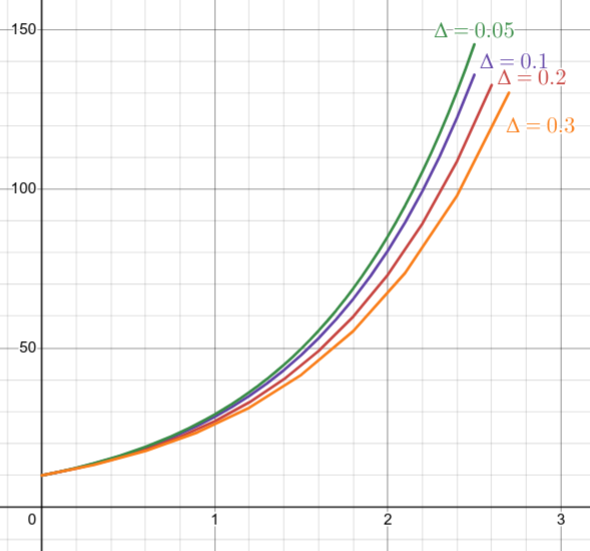
\includegraphics[width=2.5in]{compare-deltas.png}

	\begin{parts}
		\item Compare $\Delta=0.1$ and $\Delta=0.2$. Which approximation grows faster?
		\item Graph the population estimates for $\Delta=0.1$ and $\Delta=0.2$ on the same plot. What does the graph show?

		\vspace{1cm}
		\item What $\Delta$s give the largest estimate for the population at time $t$?
		\item Is there a limit as $\Delta\to 0$?
	\end{parts}
\end{slide}

\begin{slide}
	\question
	\label{many-models}
	Consider the following models for starfish growth
	\begin{itemize}
		\item[\textbf{M}] \# new children per year $\sim$ current population
		\item[\textbf{N}] \# new children per year $\sim$ current population times resources available per individual
		\item[\textbf{O}] \# new children per year $\sim$ current population times the fraction of total resources remaining
	\end{itemize}

	\begin{parts}
		\item Guess what the population vs. time curves look like for each model. \label{model-guess-part}
		\item Create a differential equation for each model.
		\item Simulate population vs. time curves for each model (but pick a common initial population).
	\end{parts}
\end{slide}

\begin{slide}
	\question
	Recall the models
	\begin{itemize}
		\item[\textbf{M}] \# new children per year $\sim$ current population
		\item[\textbf{N}] \# new children per year $\sim$ current population times resources available per individual
		\item[\textbf{O}] \# new children per year $\sim$ current population times the fraction of total resources remaining
	\end{itemize}

	\begin{parts}
		\item Determine which population grows fastest in the short term and which grows fastest in the long term.
		\item Are some models more sensitive to your choice of $\Delta$ when simulating?
		\item Are your simulations for each model consistently underestimates? Overestimates?
		\item Compare your simulated results with your guesses from question \ref{many-models}.\ref{model-guess-part}.
		What did you guess correctly? Where were you off the mark?
	\end{parts}
\end{slide}

%
% Hours 7-9
%


\begin{slide}
	\question
	A simple model for population growth has the form
	\[
		P'(t) = bP(t)
	\]
	where $b$ is the \emph{birth rate}.

	\begin{parts}
		\item Create a better model for population that includes both births and deaths.
	\end{parts}
\end{slide}

\begin{slide}
	\question
	\emph{Lotka-Volterra Predator-Prey} models predict two populations, $F$ (foxes) and $R$ (rabbits), simultaneously. They take the form
	\begin{align*}
		F'(t) &= (B_F - D_F)\cdot F(t)\\
		R'(t) &= (B_R - D_R)\cdot R(t)
	\end{align*}
	where $B_{?}$ stands for births and $D_{?}$ stands for deaths.

	We will assume:
	\vspace{-.3cm}
	\begin{itemize}
		\item Foxes die at a constant rate.
		\vspace{-.1cm}
		\item Foxes mate when food is plentiful.
		\vspace{-.1cm}
		\item Rabbits mate at a constant rate.
		\vspace{-.1cm}
		\item Foxes eat rabbits.
	\end{itemize}

	\bigskip
	\begin{parts}
		\item Speculate on when $B_F$, $D_F$, $B_R$, and $D_R$ would be at their maximum(s)/minimum(s), given our assumptions.
		\item Come up with appropriate formulas for $B_F$, $B_R$, $D_F$, and $D_R$.
	\end{parts}
	\bigskip
	\bigskip
	\bigskip
	\bigskip
	\bigskip
	\bigskip
	\phantom{x}
\end{slide}

\begin{slide}
	\question
	Suppose the population of $F$ (foxes) and $R$ (rabbits) evolves over time following the rule
	\begin{align*}
		F'(t) &= (0.01\cdot R(t) - 1.1)\cdot F(t)\\
		R'(t) &= (1.1 - 0.1\cdot F(t))\cdot R(t)
	\end{align*}

	\begin{parts}
		\item Simulate the population of foxes and rabbits with a spreadsheet.
		\item Do the populations continue to grow/shrink forever? Are they cyclic?
		\item Should the humps/valleys in the rabbit and fox populations be in phase? Out of phase?
	\end{parts}
\end{slide}

\begin{slide}
	\question
	% https://utoronto-my.sharepoint.com/:x:/g/personal/jason_siefken_utoronto_ca/Eay4QOMvy7lNr5pOKRv22NgBLGUw7qMpSCShUjeAdrhsHQ?e=bpg4CP
	Open the spreadsheet

	\url{https://uoft.me/foxes-and-rabbits}

	which contains an Euler approximation for the Foxes and Rabbits population.
	\begin{align*}
		F'(t) &= (0.01\cdot R(t) - 1.1)\cdot F(t)\\
		R'(t) &= (1.1 - 0.1\cdot F(t))\cdot R(t)
	\end{align*}

	\begin{parts}
		\item Is the max population of the rabbits over/under estimated? Sometimes over, sometimes under?
		\item What about the foxes?
		\item What about the min populations?
	\end{parts}
\end{slide}

\begin{slide}
	\question
	% https://utoronto-my.sharepoint.com/:x:/g/personal/jason_siefken_utoronto_ca/Eay4QOMvy7lNr5pOKRv22NgBLGUw7qMpSCShUjeAdrhsHQ?e=bpg4CP
	Open the spreadsheet

	\url{https://uoft.me/foxes-and-rabbits}

	which contains an Euler approximation for the Foxes and Rabbits population.
	\begin{align*}
		F'(t) &= (0.01\cdot R(t) - 1.1)\cdot F(t)\\
		R'(t) &= (1.1 - 0.1\cdot F(t))\cdot R(t)
	\end{align*}

	\SavedDefinitionRender{ComponentGraphAndPhasePlane}

	\begin{parts}
		\item Plot the Fox vs.~Rabbit population in the \emph{phase plane}. 
		\item Should your plot show a closed curve or a spiral?
		\item What ``direction'' do points move along the curve as time increases? Justify by referring to the model.
		\item What is easier to see from plots in the phase plane than from component graphs (the graphs of
		fox and rabbit population vs. time)?
	\end{parts}
\end{slide}

\begin{slide}
	\question
	% https://utoronto-my.sharepoint.com/:x:/g/personal/jason_siefken_utoronto_ca/Eay4QOMvy7lNr5pOKRv22NgBLGUw7qMpSCShUjeAdrhsHQ?e=bpg4CP
	Open the spreadsheet

	\url{https://uoft.me/foxes-and-rabbits}

	which contains an Euler approximation for the Foxes and Rabbits population.
	\begin{align*}
		F'(t) &= (0.01\cdot R(t) - 1.1)\cdot F(t)\\
		R'(t) &= (1.1 - 0.1\cdot F(t))\cdot R(t)
	\end{align*}

	\SavedDefinitionRender{EquilibriumSolution}

	\begin{parts}
		\item By changing initial conditions, what is the ``smallest'' curve you can get in the phase plane? What happens at
		those initial conditions?
		\item What should $F'$ and $R'$ be if $F$ and $R$ are \emph{equilibrium solutions}?
		\item How many equilibrium solutions are there for the fox-and-rabbit system? Justify your answer.
		\item What do the equilibrium solutions look like in the phase plane? What about their component graphs?
	\end{parts}
\end{slide}

\begin{slide}
	\question
	Recall the logistic model for starfish growth:
	\begin{itemize}
		\item[\textbf{O}] \# new children per year $\sim$ current population times the fraction of total resources remaining
	\end{itemize}
	which can be modeled with the equation
	\[
		P'(t) = k\cdot P(t)\cdot \left(1-\tfrac{R_i}{R}\cdot P(t)\right)
	\]
	where 
	\begin{itemize}
		\item $P(t)$ is the population at time $t$
		\item $k$ is a constant of proportionality 
		\item $R$ is the total number of resources
		\item $R_i$ is the resources that one starfish wants to consume
	\end{itemize}

	Use $k=1.1$, $R=1$, and $R_i=0.1$ unless instructed otherwise.

	\begin{parts}
		\item What are the equilibrium solutions for model \textbf{O}?
		\item What does a ``phase plane'' for model \textbf{O} look like? What do graphs of equilibrium solutions look like?
		\item Classify the behaviour of solutions that lie \emph{between} the equilibrium solutions. E.g., are they increasing, decreasing, oscillating?
	\end{parts}
\end{slide}

\begin{slide}
	\question

	\SavedDefinitionRender{ClassificationOfEquilibria}

	\SavedDefinitionRender{ClassificationOfEquilibriaFormal}
\end{slide}

\begin{slide}
	\SavedDefinitionRender{ClassificationOfEquilibria}

	Let
	\[
		F'(t) =\ ?
	\]
	be an unknown differential equation with equilibrium solution $f(t)=1$.

	\begin{parts}
		\item Draw an example of what solutions might look like if $f$ is \emph{attracting}.
		\item Draw an example of what solutions might look like if $f$ is \emph{repelling}.
		\item Draw an example of what solutions might look like if $f$ is \emph{stable}.
		\item Could $f$ be stable but \emph{not} attracting?
	\end{parts}
\end{slide}

\begin{slide}
	\question
	
	\SavedDefinitionRender{ClassificationOfEquilibria}
	
	Recall the starfish population model \textbf{O} given by
	\[
		P'(t) = k\cdot P(t)\cdot \left(1-\tfrac{R_i}{R}\cdot P(t)\right)
	\]
	Use $k=1.1$, $R=1$, and $R_i=0.1$ unless instructed otherwise.


	\begin{parts}
		\item Classify the equilibrium solutions for model \textbf{O} as attracting/repelling/stable/unstable/semi-stable.
		\item Does changing $k$ change the nature of the equilibrium solutions? How can you tell?
	\end{parts}
\end{slide}

%
% Hours 10-12
%

\begin{slide}
	% https://www.desmos.com/calculator/ghavqzqqjn

	\question
	
	\begin{center}
	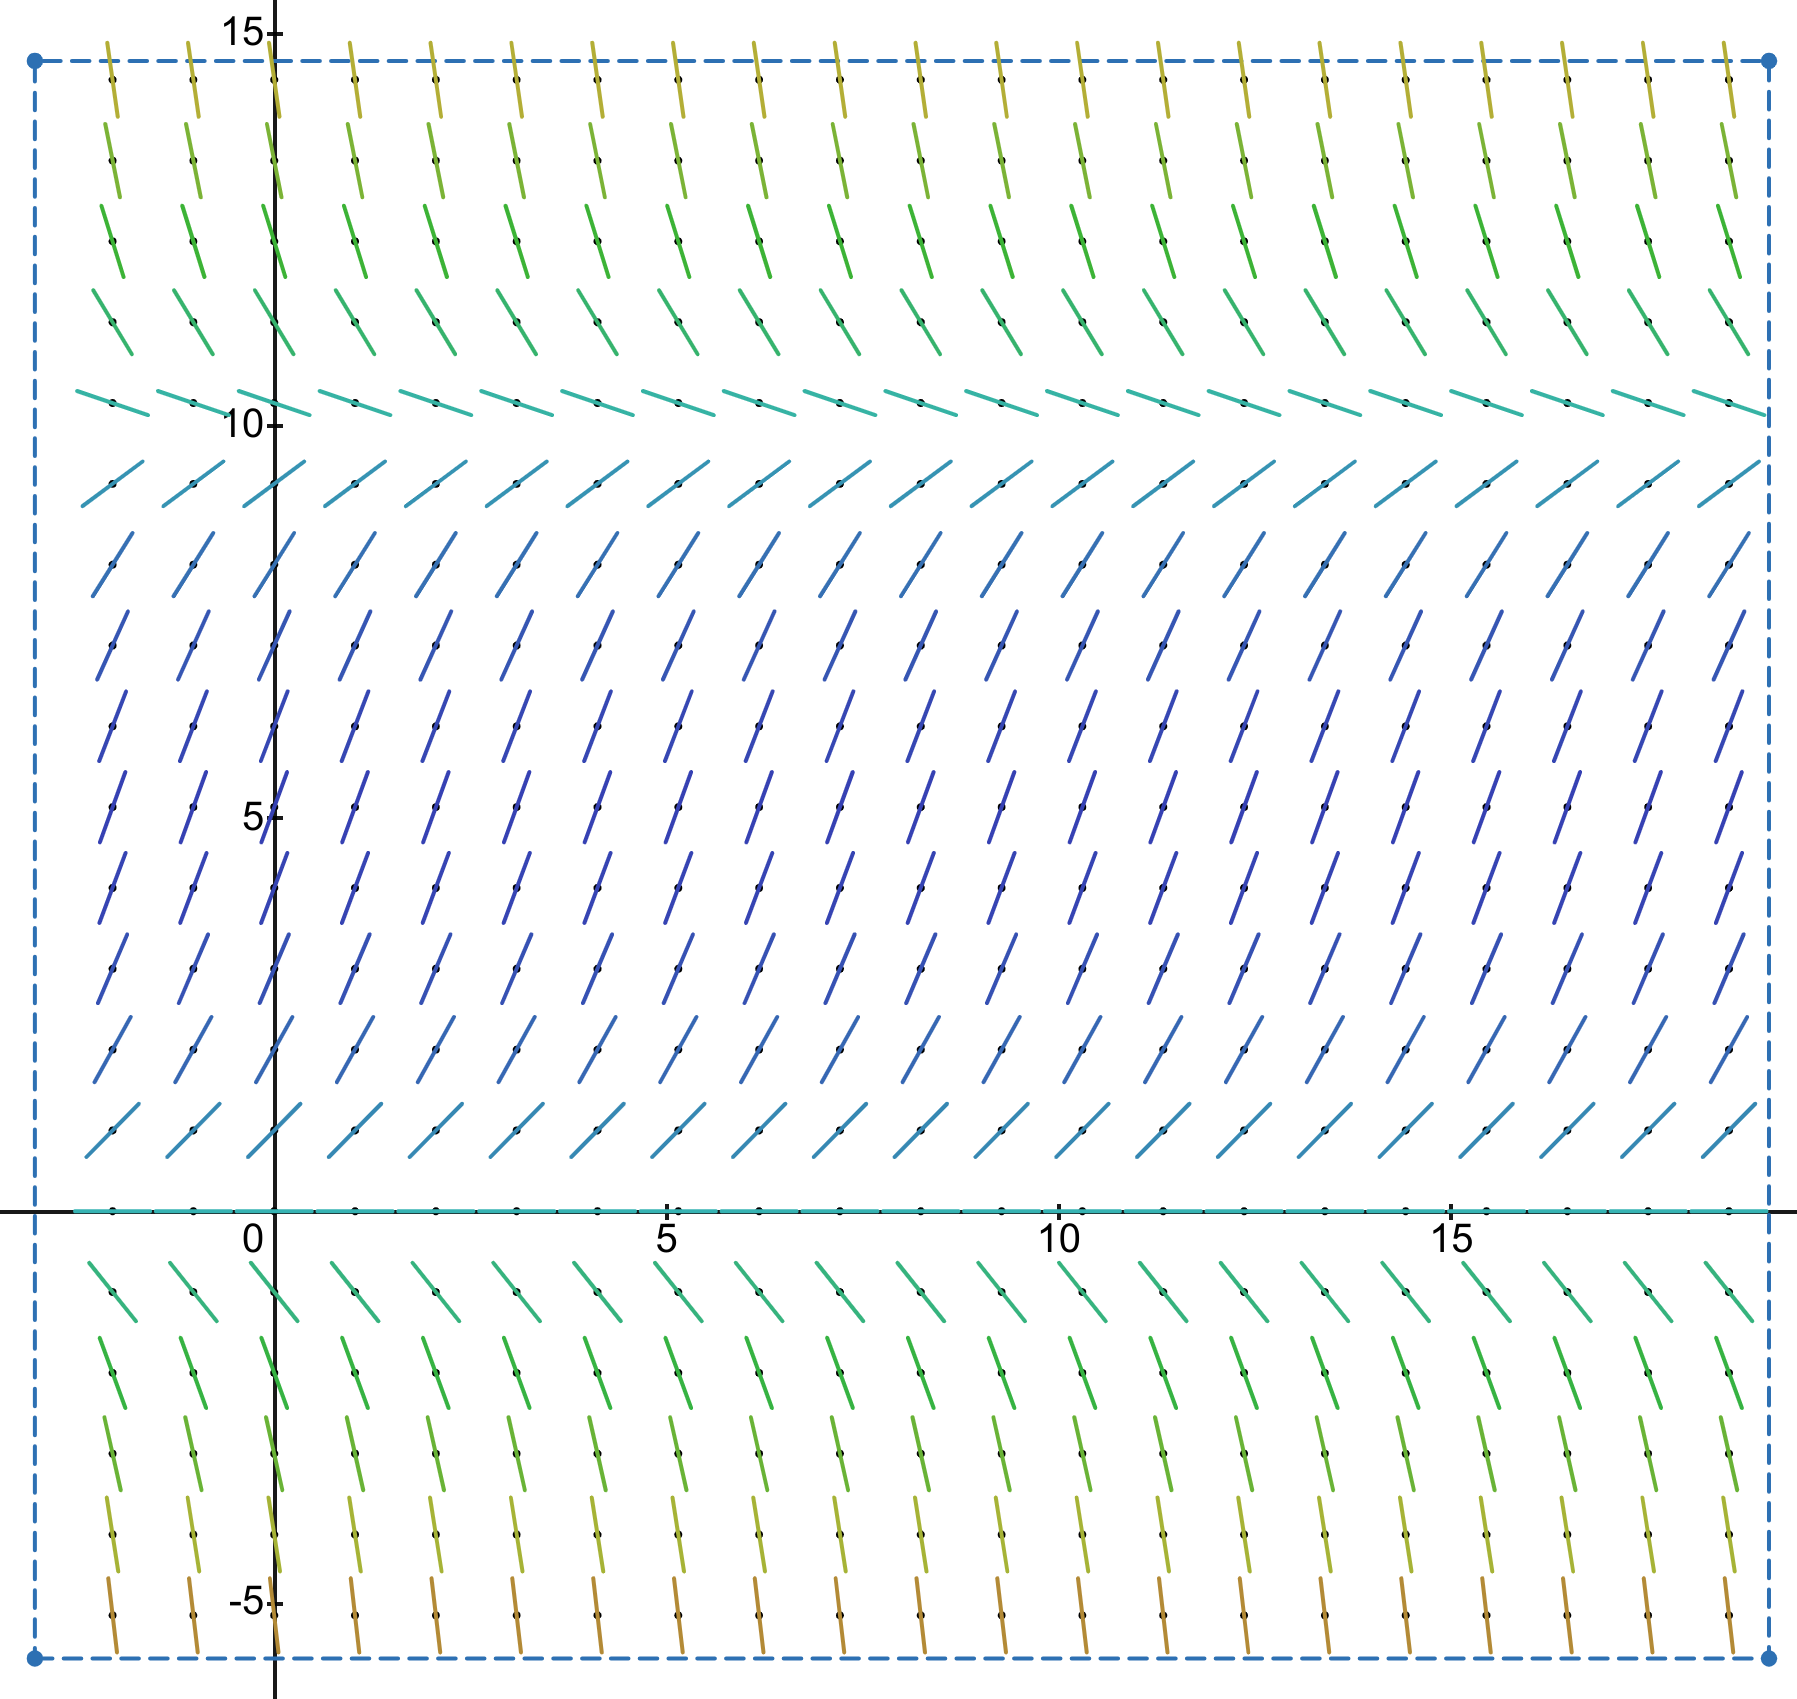
\includegraphics[width=2.5in]{slope-field-for-O.png}
	\end{center}

	A \emph{slope field} is a plot of small segments of tangent lines
	to solutions of a differential equation at different initial conditions.
	
	On the left is a slope field for model \textbf{O}, available at

	\url{https://www.desmos.com/calculator/ghavqzqqjn}

	\begin{parts}
		\item If you were sketching the slope field for model \textbf{O} by hand, what line would you sketch
		(a segment of) at $(5,3)$? Write an equation for that line.
		\item How can you recognize equilibrium solutions in a slope field?
		\item Give qualitative descriptions of different solutions to the \emph{differential equation} used in model \textbf{O} (i.e., use words to describe them). Do all
		of those solutions make sense in terms of \emph{model \textbf{O}}?
	\end{parts}
\end{slide}

\begin{slide}
	% https://www.desmos.com/3d/kvyztvmp0g

	\question
	
	\begin{center}
		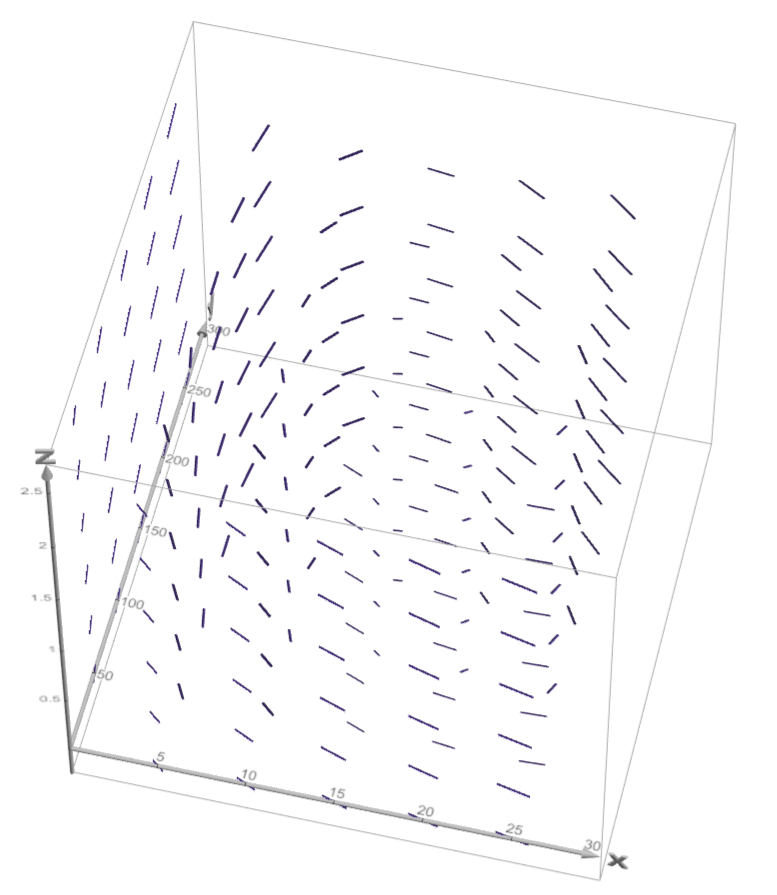
\includegraphics[width=2in]{slope-field-3d.png}
	\end{center}

	3d slope fields are possible, but hard to interpret.

	On the left is a slope field for the Foxes--Rabbits model.

	\url{https://www.desmos.com/3d/kvyztvmp0g}

	\begin{parts}
		\item What are the three dimensions in the plot?
		\item What should the graph of an equilibrium solution look like?
		\item What should the graph of a typical solution look like?
		\item What are ways to simplify the picture so we can more easily analyze solutions?
	\end{parts}
\end{slide}


\begin{slide}
	% https://www.desmos.com/calculator/wdgtznxndp
	%
	% Without Euler's built in:
	% https://www.desmos.com/calculator/vrk0q4espx

	\question
	
	\begin{center}
		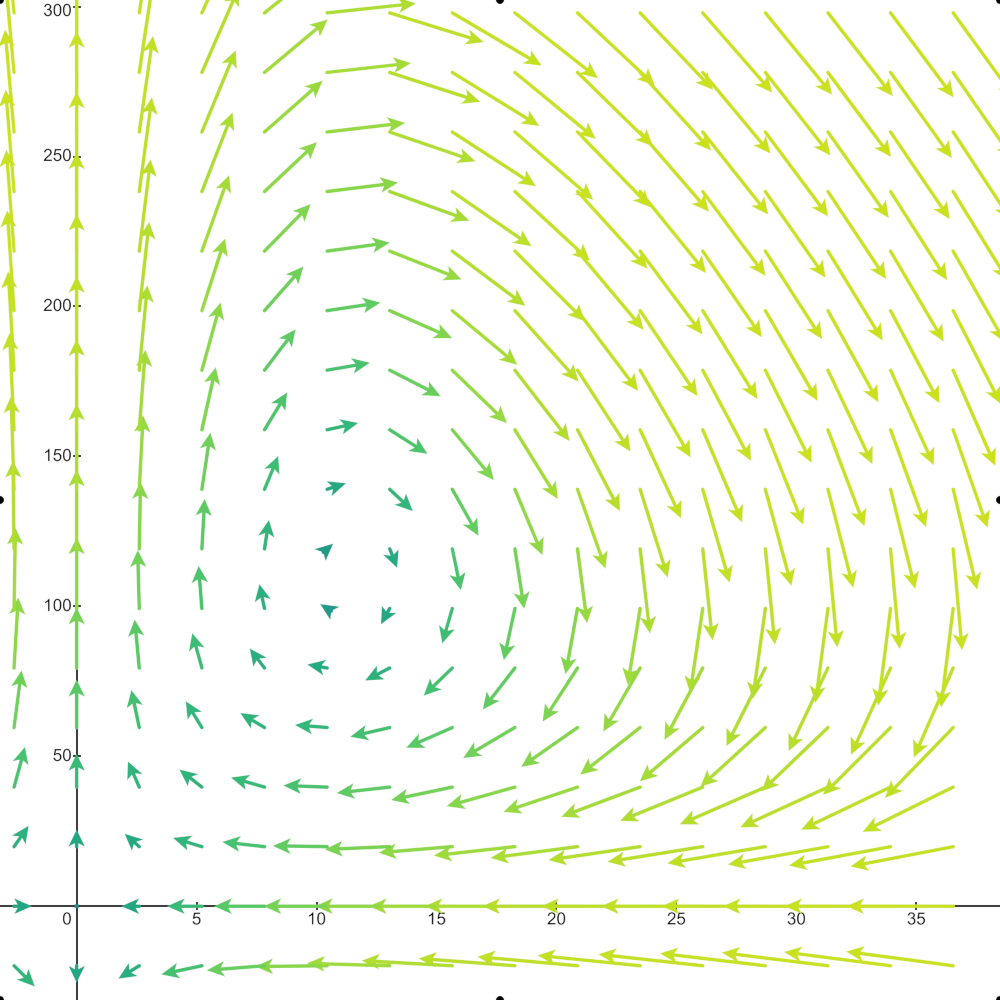
\includegraphics[width=2.5in]{phase-portrait-foxes-wolves.png}
	\end{center}


	\SavedDefinitionRender{PhasePortrait}

	On the left is a phase portrait for the Foxes--Rabbits model.

	\url{https://www.desmos.com/calculator/vrk0q4espx}

	\begin{parts}
		\item What do the $x$ and $y$ axes correspond to?
		\item Identify the equilibria in the phase portrait. What are the lengths of the vectors at those points?
		\item Classify each equilibrium as stable/unstable.
		\item Copy and paste data from your simulation spreadsheet into the Desmos plot. Does the resulting
		curve fit with the picture?
		%\item Why is the vector at $(5,100)$ longer than the vector at $(10,100)$? Justify numerically.
	\end{parts}
\end{slide}

\begin{slide}
	% https://www.desmos.com/calculator/wdgtznxndp
	%
	% Without Euler's built in:
	% https://www.desmos.com/calculator/vrk0q4espx

	\question
	Sketch your own vector field where the corresponding system of differential equations:

	\begin{parts}
		\item Has an attracting equilibrium solution.
		\item Has a repelling equilibrium solution.
		\item Has no equilibrium solutions.
	\end{parts}
\end{slide}

\begin{slide}
	% https://www.desmos.com/calculator/ghavqzqqjn

	\question
	
	\begin{center}
	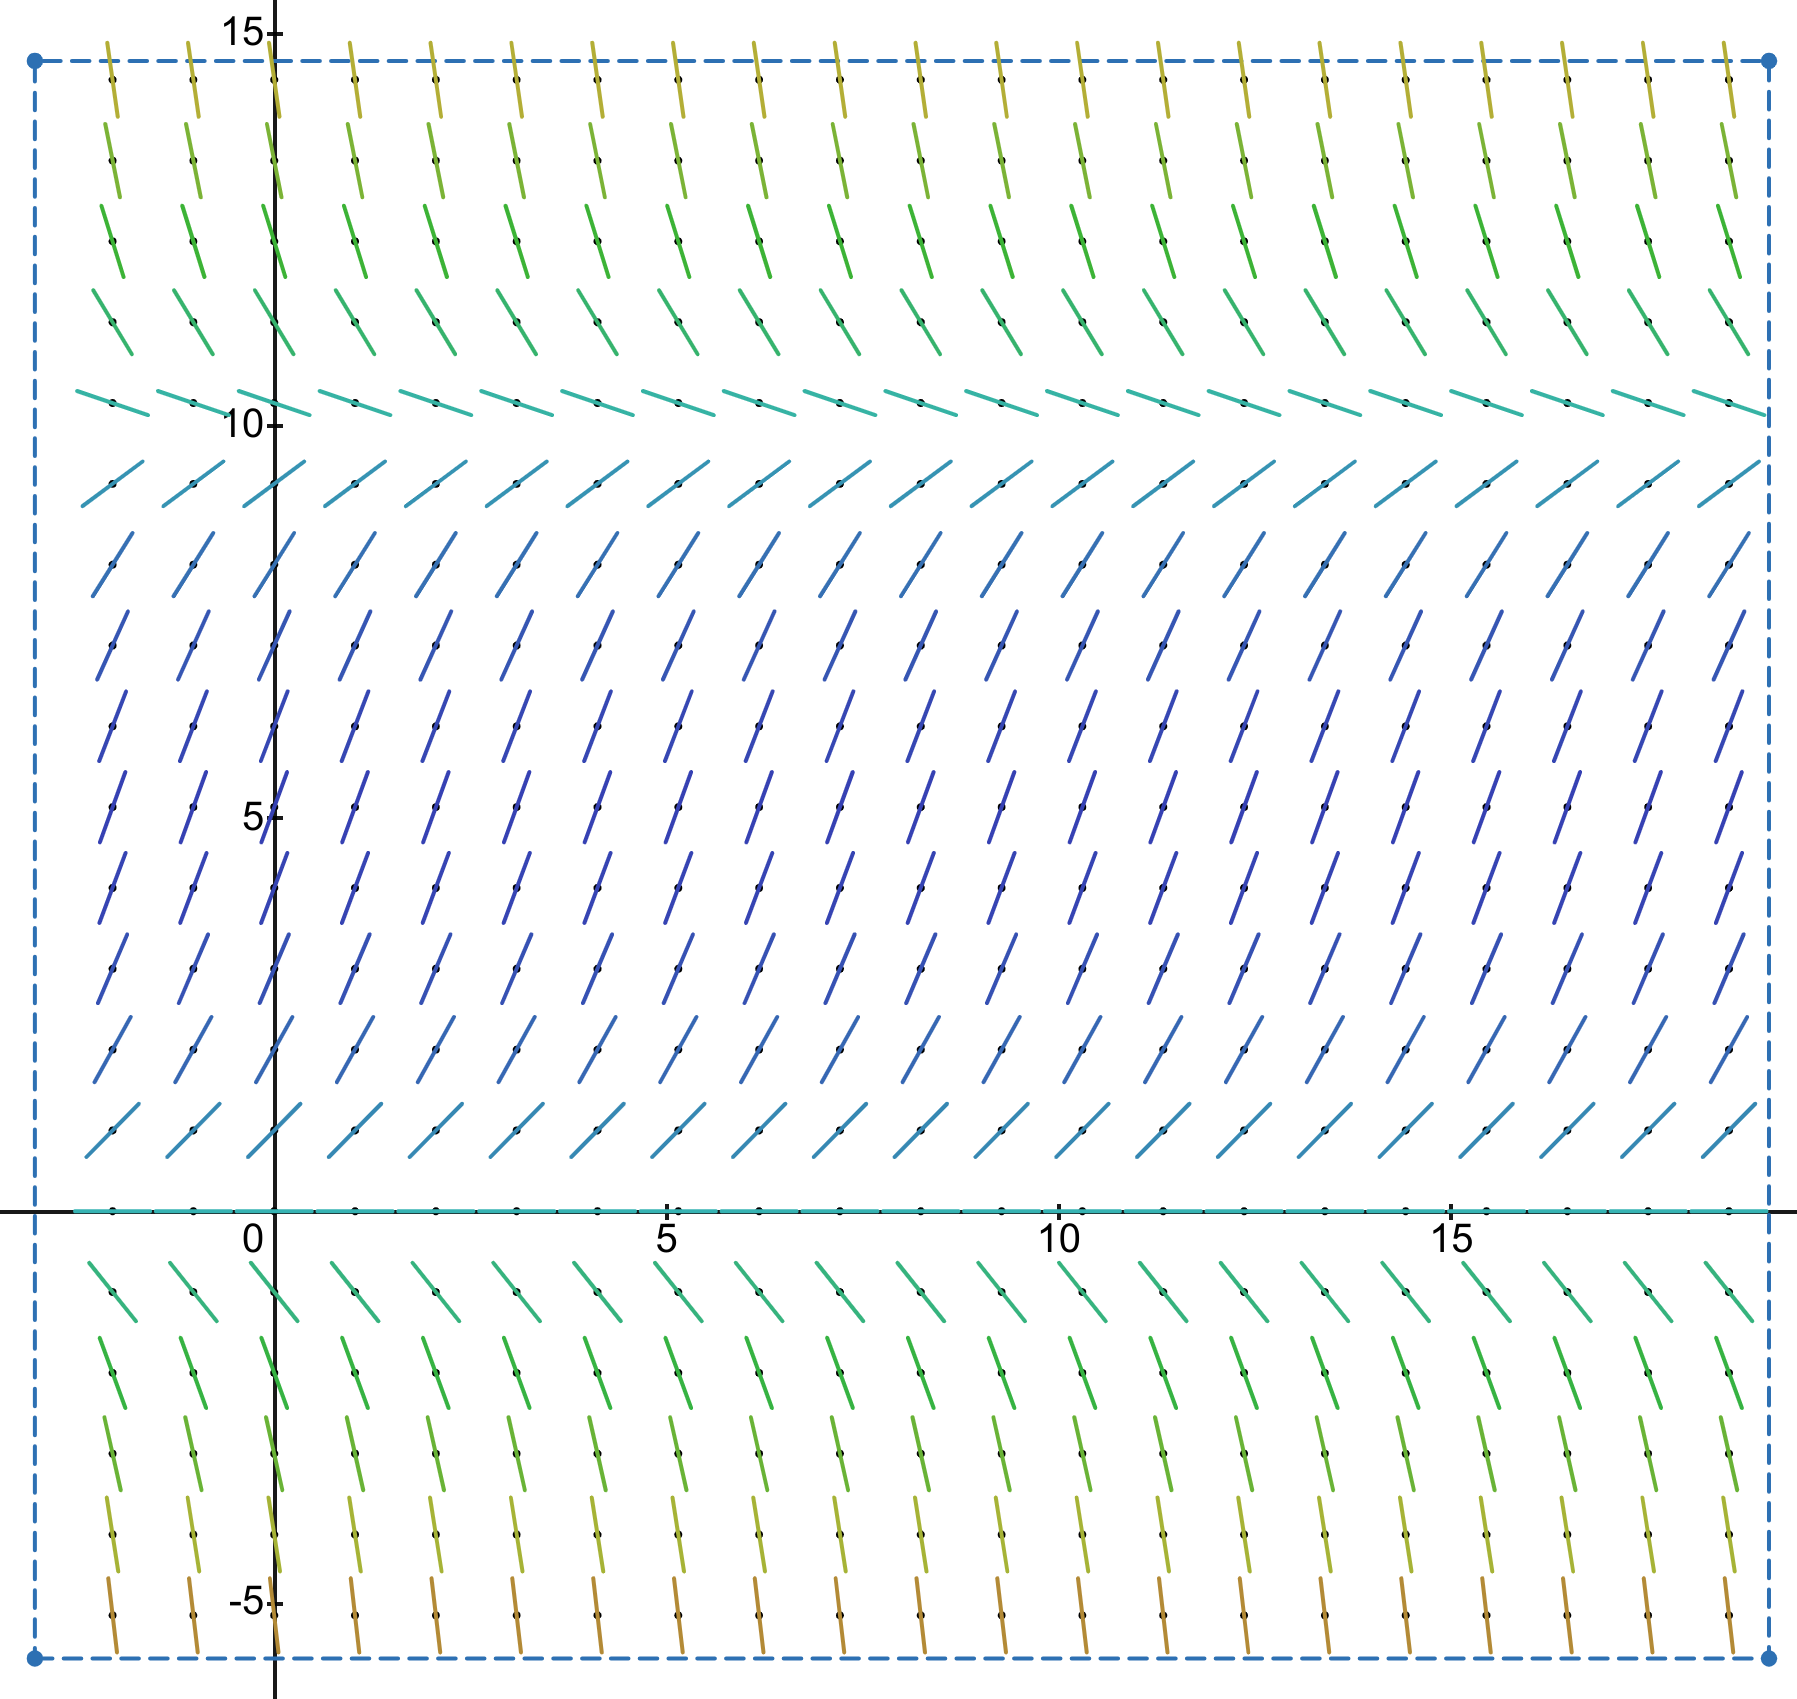
\includegraphics[width=2.5in]{slope-field-for-O.png}
	\end{center}

	Recall the slope field for model \textbf{O}.

	\begin{parts}
		\item What would a phase portrait for model \textbf{O} look like? Draw it.
		\item Where are the arrows the longest? Shortest?
		\item How could you tell from a 1d phase portrait whether an equilibrium solution is
		attracting/repelling/etc.?
	\end{parts}
\end{slide}

\begin{slide}
	%
	% Completed phase portrait in desmos:
	% https://www.desmos.com/calculator/tvjag852ja
	\question
	\label{q-phase}
	The following differential equation models the life cycle of a tree.
	In the model
	\begin{itemize}
		\item $H(t)\ =$ height (in meters) of tree trunk at time $t$
		\item $A(t)\ =$ surface area (in square meters) of all leaves at time $t$
	\end{itemize}
	\begin{align*}
		H'(t) &= 0.3\cdot A(t)-b\cdot H(t)\\
		A'(t) &= -0.3\cdot (H(t))^2 + A(t)
	\end{align*}
	and $0 \leq b \leq 2$

	\bigskip
	\phantom{x}
	\begin{parts}
		\item 
		\label{part-phase}
		Modify 

		{\small
		\url{https://www.desmos.com/calculator/vrk0q4espx}
		}

		to make a phase portrait for the tree model.
		\item What do equilibrium solutions mean in terms of tree growth?
		\item For $b=1$ what are the equilibrium solution(s)?
	\end{parts}
	\bigskip
	\phantom{x}
\end{slide}

\begin{slide}
	%
	% Completed phase portrait in desmos:
	% https://www.desmos.com/calculator/tvjag852ja
	\question
	The following differential equation models the life cycle of a tree.
	In the model
	\begin{itemize}
		\item $H(t)\ =$ height (in meters) of tree trunk at time $t$
		\item $A(t)\ =$ surface area (in square meters) of all leaves at time $t$
	\end{itemize}
	\begin{align*}
		H'(t) &= 0.3\cdot A(t)-b\cdot H(t)\\
		A'(t) &= -0.3\cdot (H(t))^2 + A(t)
	\end{align*}
	and $0 \leq b \leq 2$

	\bigskip
	\phantom{x}
	\begin{parts}
		\item Fix a value of $b$ and use a spreadsheet to simulate some solutions with different initial conditions.
		Plot the results on your phase portrait from \ref{q-phase}.\ref{part-phase}.
		\item What will happen to a tree with $(H(0), A(0))=(20,10)$? Does this depend on $b$?
		\item What will happen to a tree with $(H(0), A(0))=(10,10)$? Does this depend on $b$?
	\end{parts}
	\bigskip
	\phantom{x}
\end{slide}

\begin{slide}
	\question
	The tree model
	\begin{align*}
		H'(t) &= 0.3\cdot A(t)-b\cdot H(t)\\
		A'(t) &= -0.3\cdot (H(t))^2 + A(t)
	\end{align*}
	was based on the premises
	\begin{itemize}[leftmargin=3em]
		\item[ $P_{\text{height 1}}$] CO$_2$ is absorbed by the leaves and turned directly into trunk height.
		\item[ $P_{\text{height 2}}$] The tree is in a swamp and constantly sinks at a speed proportional to its height.
		\item[ $P_{\text{leaves 1}}$] Leaves grow proportionality to the energy available.
		\item[ $P_{\text{energy 1}}$] The tree gains energy from the sun proportionally to the leaf area.
		\item[ $P_{\text{energy 2}}$] The tree loses energy proportionally to the square of its height.
		%\item[ $P_{\text{energy 1}}$] The tree absorbs energy from the sun proportionality to the leaf area.
		%\item[ $P_{\text{energy 2}}$] It costs energy proportional to the square of the height for the tree to maintain its current size.
	\end{itemize}

	\begin{parts}
		\item How are the premises expressed in the differential equations?
		\item What does the parameter $b$ represent (in the real world)?
		\item Applying Euler's method to this system shows solutions that pass from the 1st to 4th quadrants of the phase plane.
			Is this realistic? Describe the life cycle of such a tree?
	\end{parts}
\end{slide}

\begin{slide}
	\question
	Recall the tree model
	\begin{align*}
		H'(t) &= 0.3\cdot A(t)-b\cdot H(t)\\
		A'(t) &= -0.3\cdot (H(t))^2 + A(t)
	\end{align*}

	\begin{parts}
		\item Find all equilibrium solutions for $0\leq b\leq 2$.
		\item For which $b$ does a tree have the possibility of living forever? If the wind occasionally blew off a few random leaves,
		would that change your answer?
		\item
		Find a value $b_5$ of $b$ so that there is an equilibrium with $H=5$.

		Find a value $b_{12}$ of $b$ so that there is an equilibrium with $H=12$.
		
		\item
		Predict what happens to a tree near equilibrium in condition $b_5$ and a tree near equilibrium in condition $b_{12}$.

	\end{parts}
\end{slide}

%
% Hours 13-14
%

\begin{slide}
	\question
	Consider the system of differential equations
	\begin{align*}
		x'(t) &= x(t)\\
		y'(t) &= 2y(t)
	\end{align*}

	\begin{parts}
		\item Make a phase portrait for the system.

		{\small \url{https://www.desmos.com/calculator/h3wtwjghv0}}
		\item What are the equilibrium solution(s) of the system?
		\item 
		Find a formula for $x(t)$ and $y(t)$ that satisfy the initial conditions $(x(0), y(0))=(x_0, y_0)$.
		\item Let $\vec r(t)=(x(t),y(t))$. Find a matrix $A$ so that the differential equation can be equivalently expressed
		as
		\[
			\vec r'(t) = A\,\vec r(t).
		\]
		\item Write a solution to $\vec r' = A\,\vec r$ (where $A$ is the matrix you came up with).
	\end{parts}
\end{slide}


\begin{slide}
	\question
	Let $A$ be an unknown matrix and suppose $\vec p$ and $\vec q$ are solutions to $\vec r'=A\,\vec r$.

	\begin{parts}
		\item Is $\vec s(t)=\vec p(t)+\vec q(t)$ a solution to $\vec r'=A\,\vec r$? Justify your answer.
		\item Can you construct other solutions from $\vec p$ and $\vec q$? If yes, how so?
	\end{parts}
\end{slide}

\begin{slide}
	\question
	Recall from MAT223:
	\SavedDefinitionRender{LinearlyDependentIndependentAlgebraic}

	Define
	\[
		\vec p(t) = \mat{e^t\\0}\qquad
		\vec q(t) = \mat{4e^t\\0}\qquad
		\vec h(t) = \mat{0\\ e^{2t}}\qquad
		\vec z(t) = \mat{0\\ e^{3t}}.
	\]


	\begin{parts}
		\item Are $\vec p$ and $\vec q$ linearly independent or linearly dependent? Justify with the definition.
		\item Are $\vec p$ and $\vec h$ linearly independent or linearly dependent? Justify with the definition.
		\item Are $\vec h$ and $\vec z$ linearly independent or linearly dependent? Justify with the definition.
		\item Is the set of three functions  $\Set{\vec p,\vec h,\vec z}$ linearly independent or linearly dependent? Justify with the definition.
	\end{parts}
\end{slide}

\begin{slide}
	\question
	Recall
	\[
		\vec p(t) = \mat{e^t\\0}\qquad
		\vec q(t) = \mat{4e^t\\0}\qquad
		\vec h(t) = \mat{0\\ e^{2t}}\qquad
		\vec z(t) = \mat{0\\ e^{3t}}.
	\]


	\begin{parts}
		\item Describe $\Span\Set{\vec p, \vec h}$. What is its dimension? What is a basis for it?
		\item Let $S$ be the set of all solutions to $\vec r'(t) = \mat{1&0\\0&2}\vec r(t)$. {
		\small(You've seen this equation before.)}

		Is $S$ a subspace? If so, what is its dimension?
		\item Provided $S$ is a subspace, give a basis for $S$.
	\end{parts}
\end{slide}

\begin{slide}
	\question
	Consider the differential equation
	\[
		y'(t) = 2\cdot y(t).
	\]


	\begin{parts}
		\item Write a solution whose graph passes through the point $(t,y)=(0,3)$.
		\item Write a solution whose graph passes through the point $(t,y)=(0,y_0)$.
		\item Write a solution whose graph passes through the point $(t,y)=(t_0,y_0)$.
		\item Consider the following argument:
		\begin{quote}
			For every point $(t_0, y_0)$, there is a corresponding solution to $y'(t) = 2\cdot y(t)$.

			Since $\Set{(t_0,y_0):t_0,y_0\in \R}$ is two dimensional, this means the set of solutions
			to $y'(t) = 2\cdot y(t)$ is two dimensional.
		\end{quote}
		Do you agree? Explain.

	\end{parts}
\end{slide}

\begin{slide}
	\question
	%\begin{theorem}
	%	For an \emph{autonomous} ordinary differential equation (whose solutions are defined on all of $\R$),
	%	a solution that passes through $(t_0, y_0)$ also passes through $(0,y_0^*)$ for some $y_0^*$.
	%\end{theorem}
	\begin{theorem}[(Existence \& Uniqueness 1)]
		The system of differential equations represented by
		 $\vec r\,'(t) = M \vec r(t) + \vec p$ (or the single differential equation 
		 $y'=ay+b$) has a unique solution passing through every initial condition. Further, the domain of every
		solution is $\R$.
	\end{theorem}

	Let $S$ be the set of all solutions to $\vec r'(t) = \mat{1&0\\0&2}\vec r(t)$.

	\begin{parts}
		\item Show that $\Dim(S) \geq 2$ by finding at least two linearly independent solutions.
		\item Let $I$ be the set of all initial conditions. What is $I$?
		\item Show that $\Dim(S) \leq 3$ by applying the theorem to the set of initial conditions.
		\item Can two points in $I$ correspond to the same solution? Explain?
		\item Find a subset $U\subseteq I$ so that every solution corresponds to a unique point in $U$.
		\item Show that $\Dim(S) \leq 2$.
		\item Suppose $M$ is an $n\times n$ matrix. Consider the differential equation
		$\vec r\,'(t)=M\vec r(t)$. If you have found $n$ linearly
		independent solutions, can you determine the dimension of the set of all solutions?
		Explain. 
	\end{parts}
\end{slide}

%
% Hours 15-18
%

\begin{slide}
	\question
	\label{qeignsoln}
	Consider the system
	\begin{align*}
		x'(t) &= 2x(t)\\
		y'(t) &= 3y(t)
	\end{align*}

	\begin{parts}
		\item Rewrite the system in matrix form.
		\item 
		\label{eigsoln}
		Classify the following as solutions or non-solutions to the system.
		\begin{align*}
			\vec r_1(t) &= e^{2t} &\qquad			\vec r_2(t) &= \mat{e^{2t}\\0}\\
			\vec r_3(t) &= \mat{e^{2t}\\4e^{3t}} &\qquad			\vec r_4(t) &= \mat{4e^{3t}\\e^{2t}}\\
			\vec r_5(t) &= \mat{0\\0}
		\end{align*}
		\item State the definition of an eigenvector for the matrix $M$.
		\item What should the definition of an \emph{eigen solution} be for this system?
		\item Which functions from \ref{qeignsoln}.\ref{eigsoln} are eigen solutions?
		\item Find an eigen solution $\vec r_6$ that is linearly independent from $\vec r_2$.
		\item Let $S=\Span\{\vec r_2, \vec r_6\}$. Does $S$ contain \emph{all} solutions to the system? Justify your answer.
	
	\end{parts}
\end{slide}

\begin{slide}
	\question
	Recall the system
	\begin{align*}
		x'(t) &= 2x(t)\\
		y'(t) &= 3y(t)
	\end{align*}
	has eigen solutions $\vec r_2(t)=\mat{e^{2t}\\0}$ and $\vec r_6(t)=\mat{0\\e^{3t}}$.

	\begin{parts}
		\item Sketch $\vec r_2$ and $\vec r_6$ in the phase plane.
		\item Use

		\url{https://www.desmos.com/calculator/h3wtwjghv0}

		to make a phase portrait for the system.

		\item 	
		\begin{minipage}[t]{.45\textwidth}
		\begin{center}
			\begin{tikzpicture}[scale=1.2, baseline=(current bounding box.north)]
					\begin{axis}[
						width=4cm,
						height=4cm,
						xmin=-.5,xmax=3.5,ymin=-.5,
						ymax=3.5, xmajorgrids, ymajorgrids,
						xtick={-4,...,4}, ytick={-4,...,4}, axis lines=middle, yticklabels={,,}, xticklabels={,,},
						samples=50, domain=0:5]
						
						\addplot[blue, mark=none] coordinates {(0,0) (0,10)};
						\addplot[red] {0};
						\addplot[forestgreen, thick, dashed, dash pattern=on 3pt off 1pt] {x^(2/3)};
					\end{axis}
			\end{tikzpicture}%
			~~~~~\begin{tikzpicture}[scale=1.2, baseline=(current bounding box.north)]
					\begin{axis}[
						width=4cm,
						height=4cm,
						xmin=-.5,xmax=3.5,ymin=-.5,
						ymax=3.5, xmajorgrids, ymajorgrids,
						xtick={-4,...,4}, ytick={-4,...,4}, axis lines=middle, yticklabels={,,}, xticklabels={,,},
						samples=50, domain=0:5]
						
						\addplot[blue, mark=none] coordinates {(0,0) (0,10)};
						\addplot[red] {0};
						\addplot[forestgreen, thick, dashed, dash pattern=on 3pt off 1pt] {x^(3/2)};
					\end{axis}
			\end{tikzpicture}\\
			\begin{tikzpicture}[scale=1.2, baseline=(current bounding box.north)]
					\begin{axis}[
						width=4cm,
						height=4cm,
						xmin=-.5,xmax=3.5,ymin=-.5,
						ymax=3.5, xmajorgrids, ymajorgrids,
						xtick={-4,...,4}, ytick={-4,...,4}, axis lines=middle, yticklabels={,,}, xticklabels={,,},
						samples=50, domain=0:5]
						
						\addplot[blue, mark=none] coordinates {(0,0) (0,10)};
						\addplot[red] {0};
						\addplot[forestgreen, thick, dashed, dash pattern=on 3pt off 1pt] {1.5*x};
					\end{axis}
			\end{tikzpicture}\\
			\end{center}
		\end{minipage}
			In which phase plane above is the dashed (green) curve the graph of a solution to the system? Explain.

		%\item Should graphs of solutions in the phase plane extend to other quadrants, or should every graph occupy only one quadrant?

	\end{parts}
\end{slide}

\begin{slide}
	\question
		Suppose $A$ is a $2\times 2$ matrix and $\vec s_1$ and $\vec s_2$ are eigen solutions to $\vec r'=A\,\vec r$ with eigenvalues $1$ and $-1$, respectively.
	\begin{parts}
		\item Write possible formulas for $\vec s_1(t)$ and $\vec s_2(t)$.
		\item Sketch a phase plane with graphs of $\vec s_1$ and $\vec s_2$ on it.
		\item Add a non-eigen solution to your sketch.
		\item Sketch a possible phase portrait for $\vec r'=A\,\vec r$. Can you extend your phase portrait to all quadrants?
	\end{parts}
\end{slide}

\begin{slide}
	\question
		Consider the following phase portrait for a system of the form $\vec r'=A\,\vec r$
		for an unknown matrix $A$.

		\begin{center}
		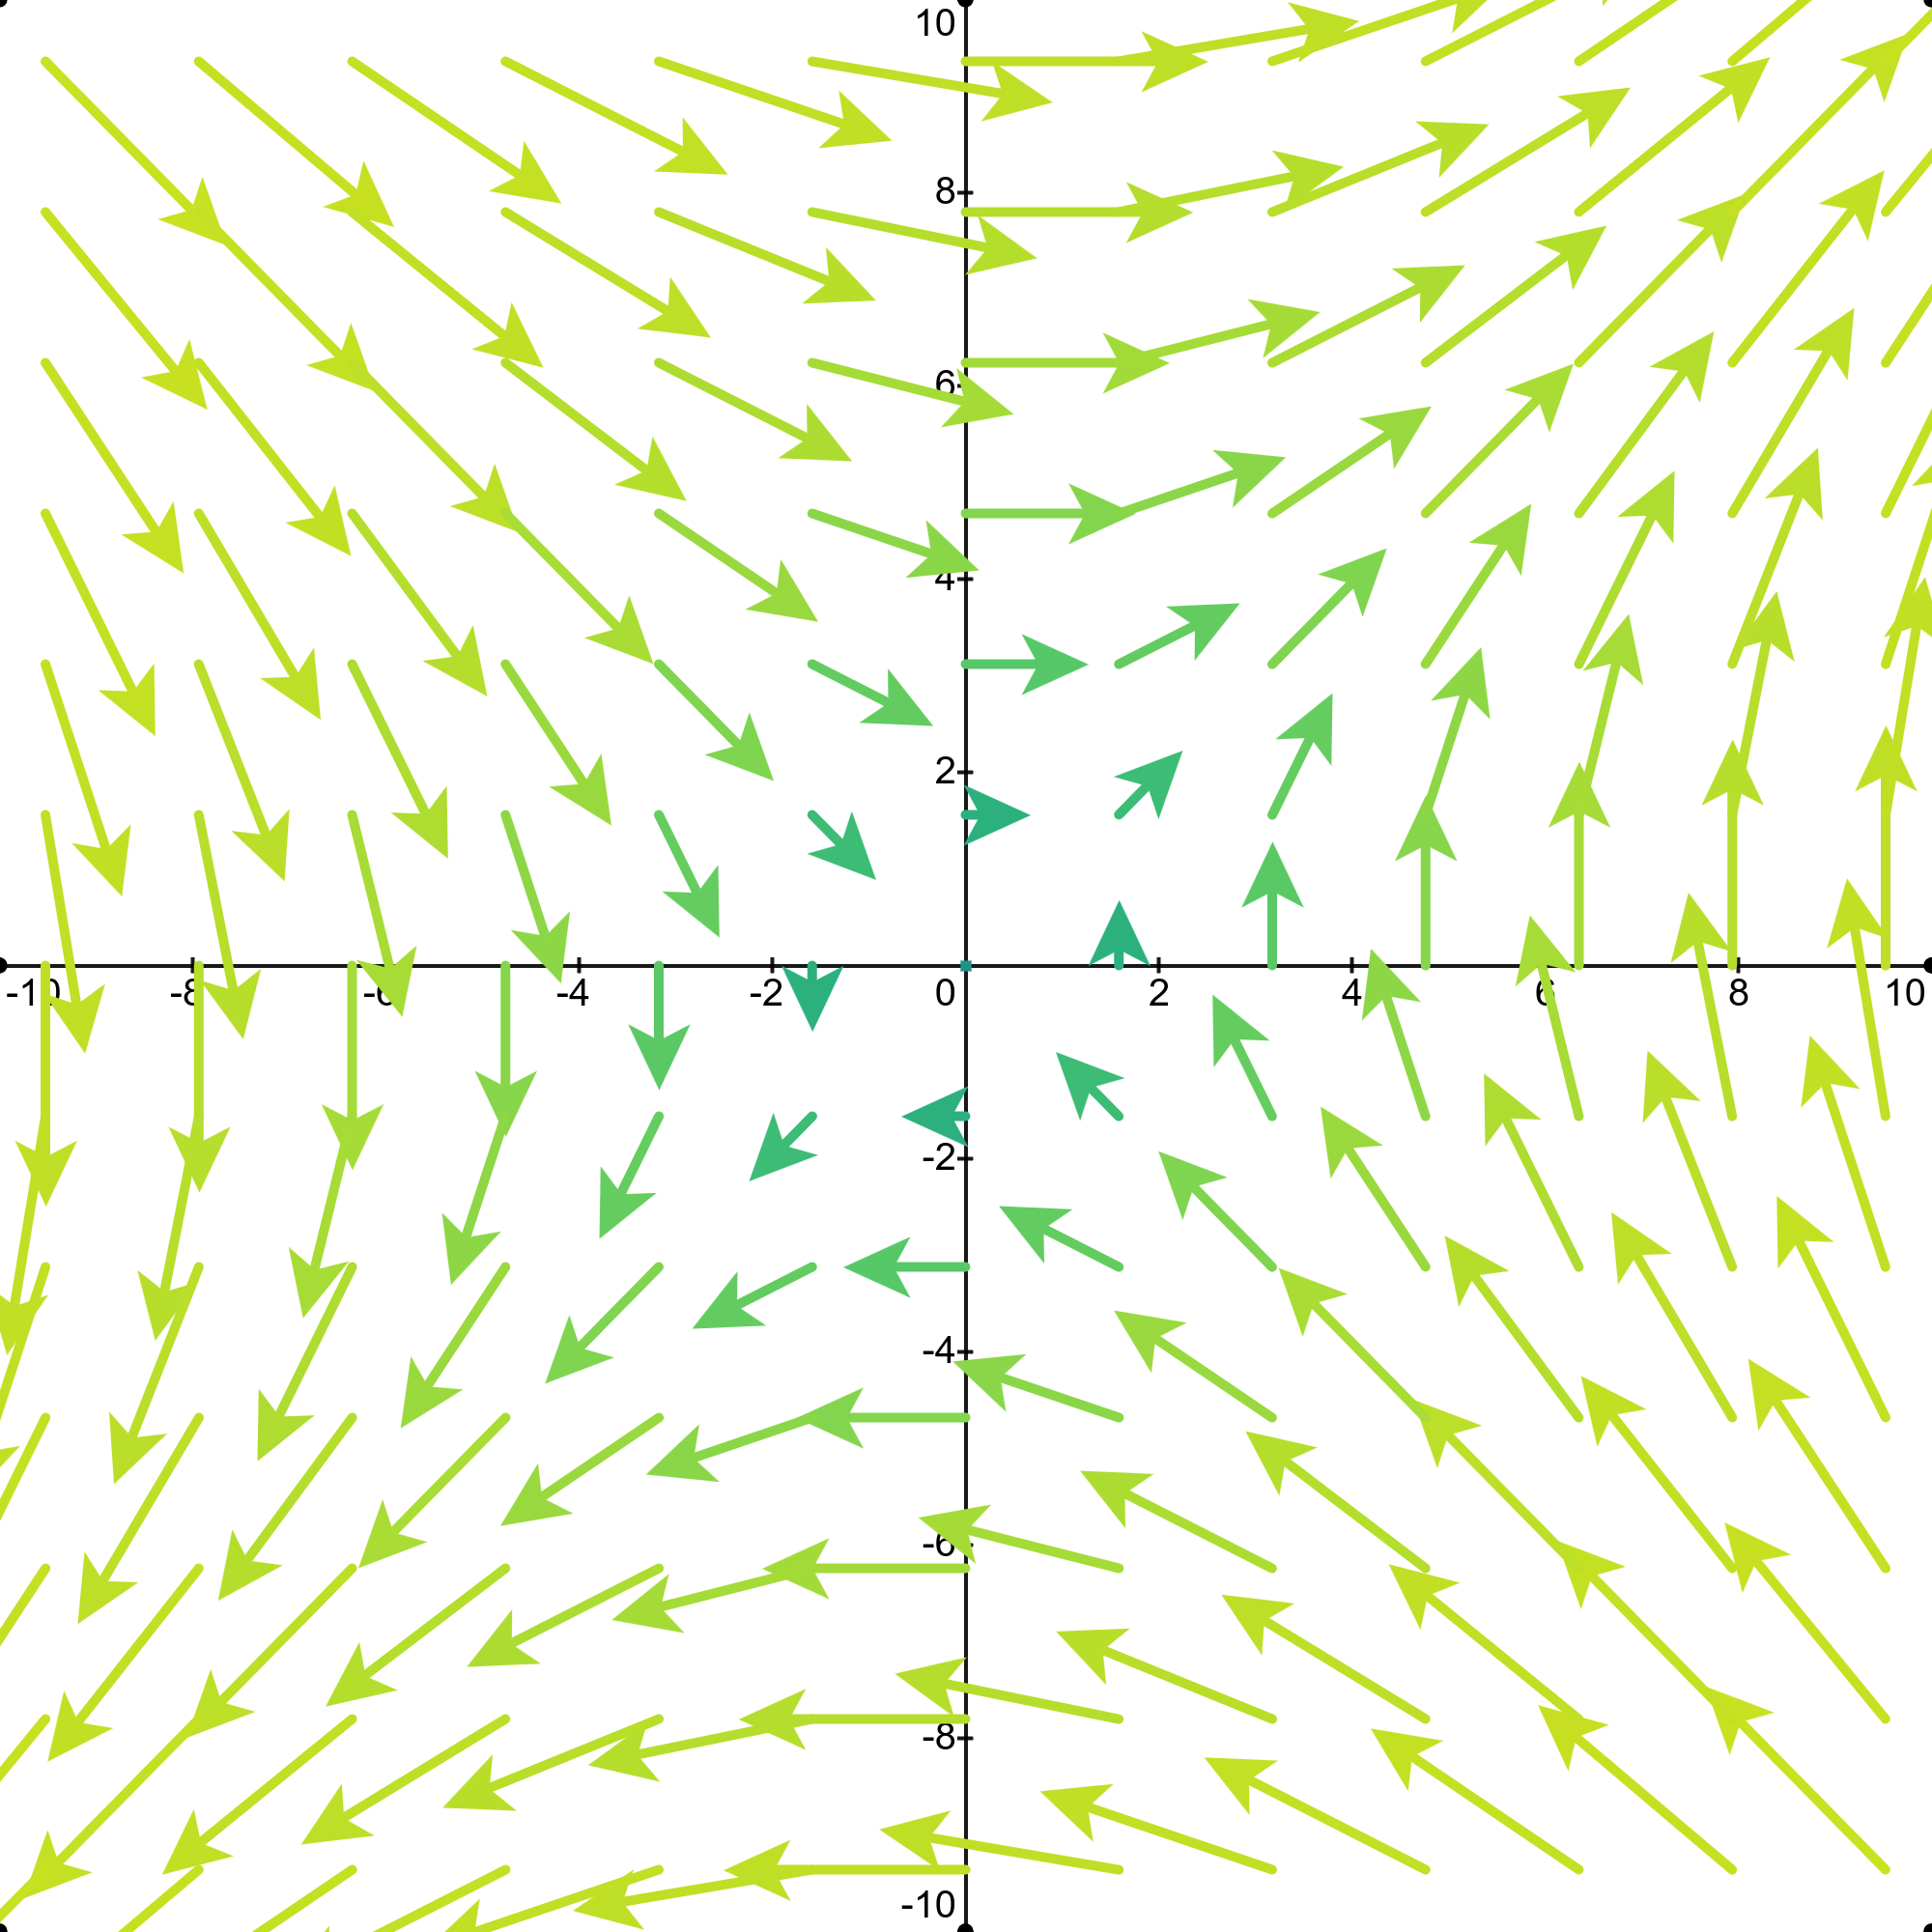
\includegraphics[width=2in]{slope-field-eig-pm-one.png}
		\end{center}
	\begin{parts}
		\item Can you identify any eigen solutions?
		\item What are the eigenvalues of $A$? What are their sign(s)?
	\end{parts}
\end{slide}

\begin{slide}
	\question
	Consider the differential equation $\vec r'(t) = M\,\vec r(t)$ where $M=\mat{0&1\\1&0}$.

	\begin{parts}
		%\item Find the eigenvectors and eigenvalues for $M$.
		\item Verify that $\mat{1\\1}$ and $\mat{1\\-1}$ are eigenvectors for $M$. What are the
		corresponding eigenvalues?
		\item 
		\begin{enumerate}
			\item Is $\vec r_1(t) =e^t \mat{1\\0}$ a solution to the differential equation? An eigen solution?
			\item Is $\vec r_2(t) =e^t \mat{1\\1}$ a solution to the differential equation? An eigen solution?
			\item Is $\vec r_3(t) =e^{2t} \mat{1\\-1}$ a solution to the differential equation? An eigen solution?
		\end{enumerate}

		\item Find an eigen solution for the system corresponding to the eigenvalue $-1$. Write your answer
		in vector form.

		\item Let $\vec v$ is an eigenvector for $M$ with eigenvalue $\lambda$. Explain how to write down an eigen solution
		to $\vec r'(t) = M\,\vec r(t)$ with eigenvalue $\lambda$.

		\item Let $\vec v\neq \vec 0$ be a non-eigenvector for $M$. Could $\vec r(t)=e^{\lambda t}\vec v$ be a solution
		to $\vec r'(t) = M\,\vec r(t)$ for some $\lambda$? Explain.
	\end{parts}
\end{slide}

\begin{slide}
	\question
	Recall the differential equation $\vec r'(t) = M\,\vec r(t)$ where $M=\mat{0&1\\1&0}$.

	\begin{parts}
		\item Write down a general solution to the differential equation.
		\item Write down a solution to the initial value problem $\vec r(0)=\mat{x_0\\y_0}$.
		\item Are your answers to the first two parts the same? Do they contain the same information?
	\end{parts}
\end{slide}

\begin{slide}
	\question
	The phase portrait for a differential equation arising from the matrix $\mat{0&1\\1&0}$ (left)
	and $\mat{1&0\\0&-1}$ (right) are shown.
	\begin{center}
		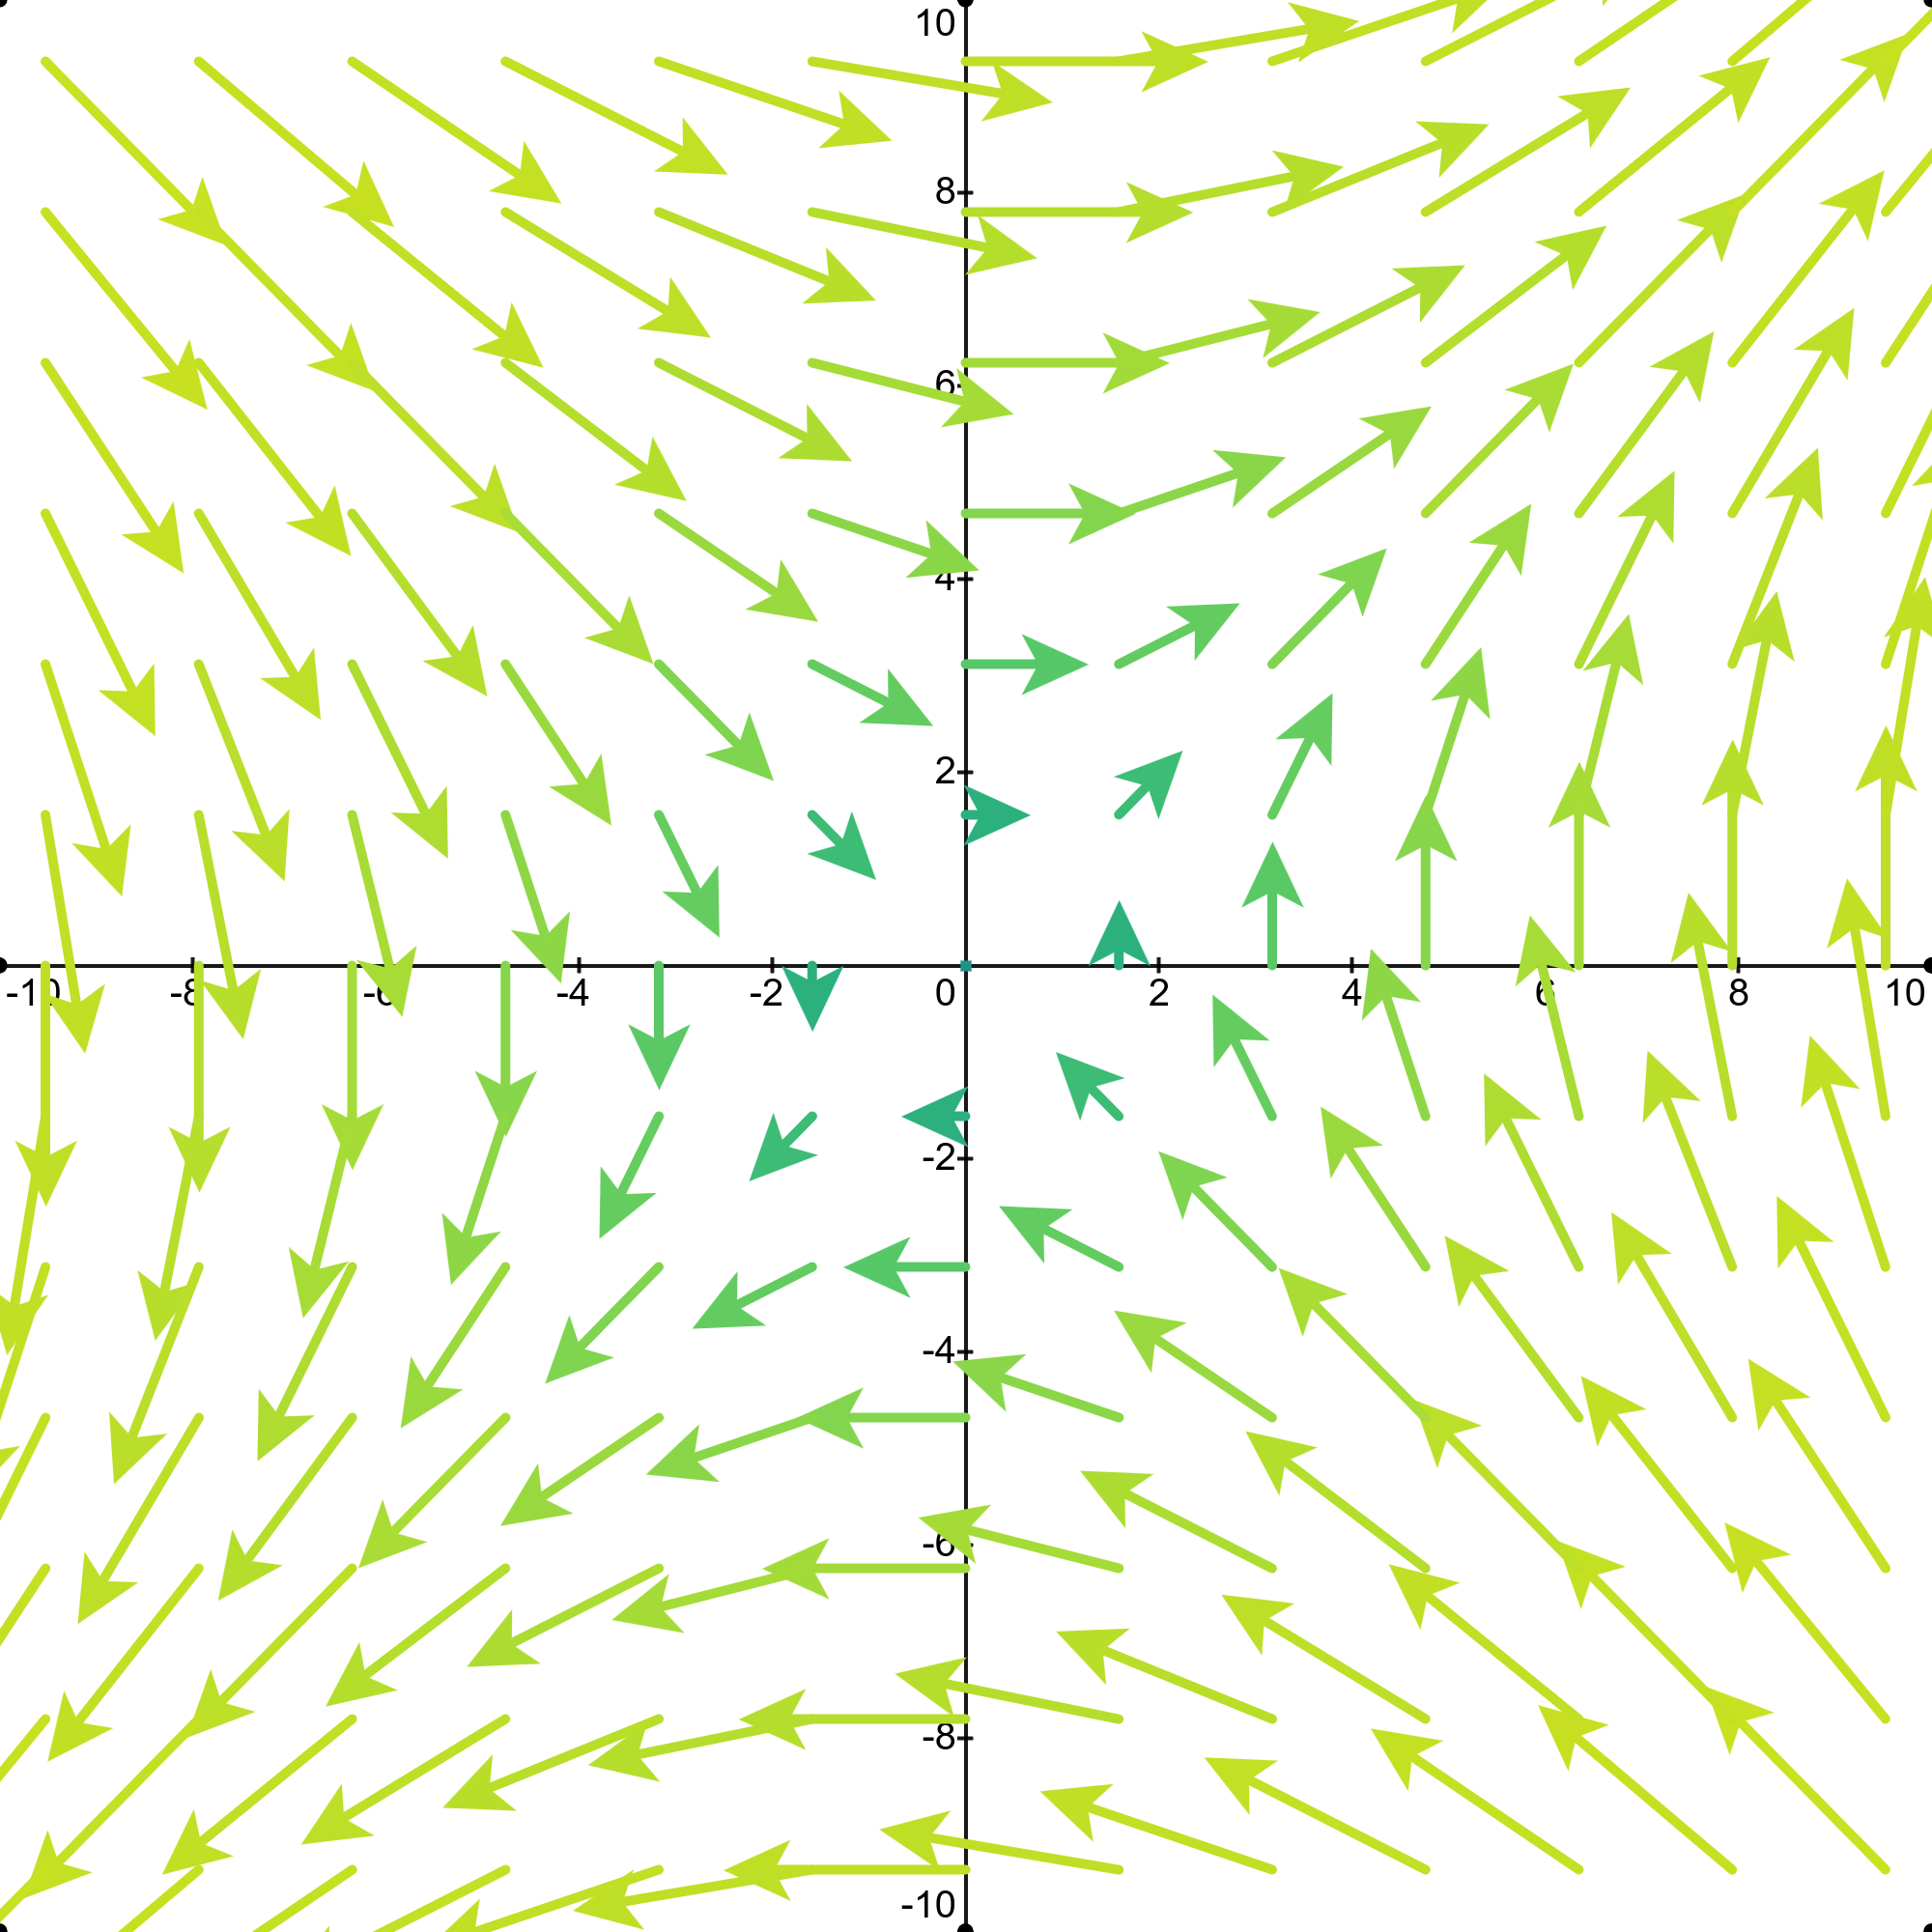
\includegraphics[width=1.7in]{slope-field-eig-pm-one.png}~~~~
		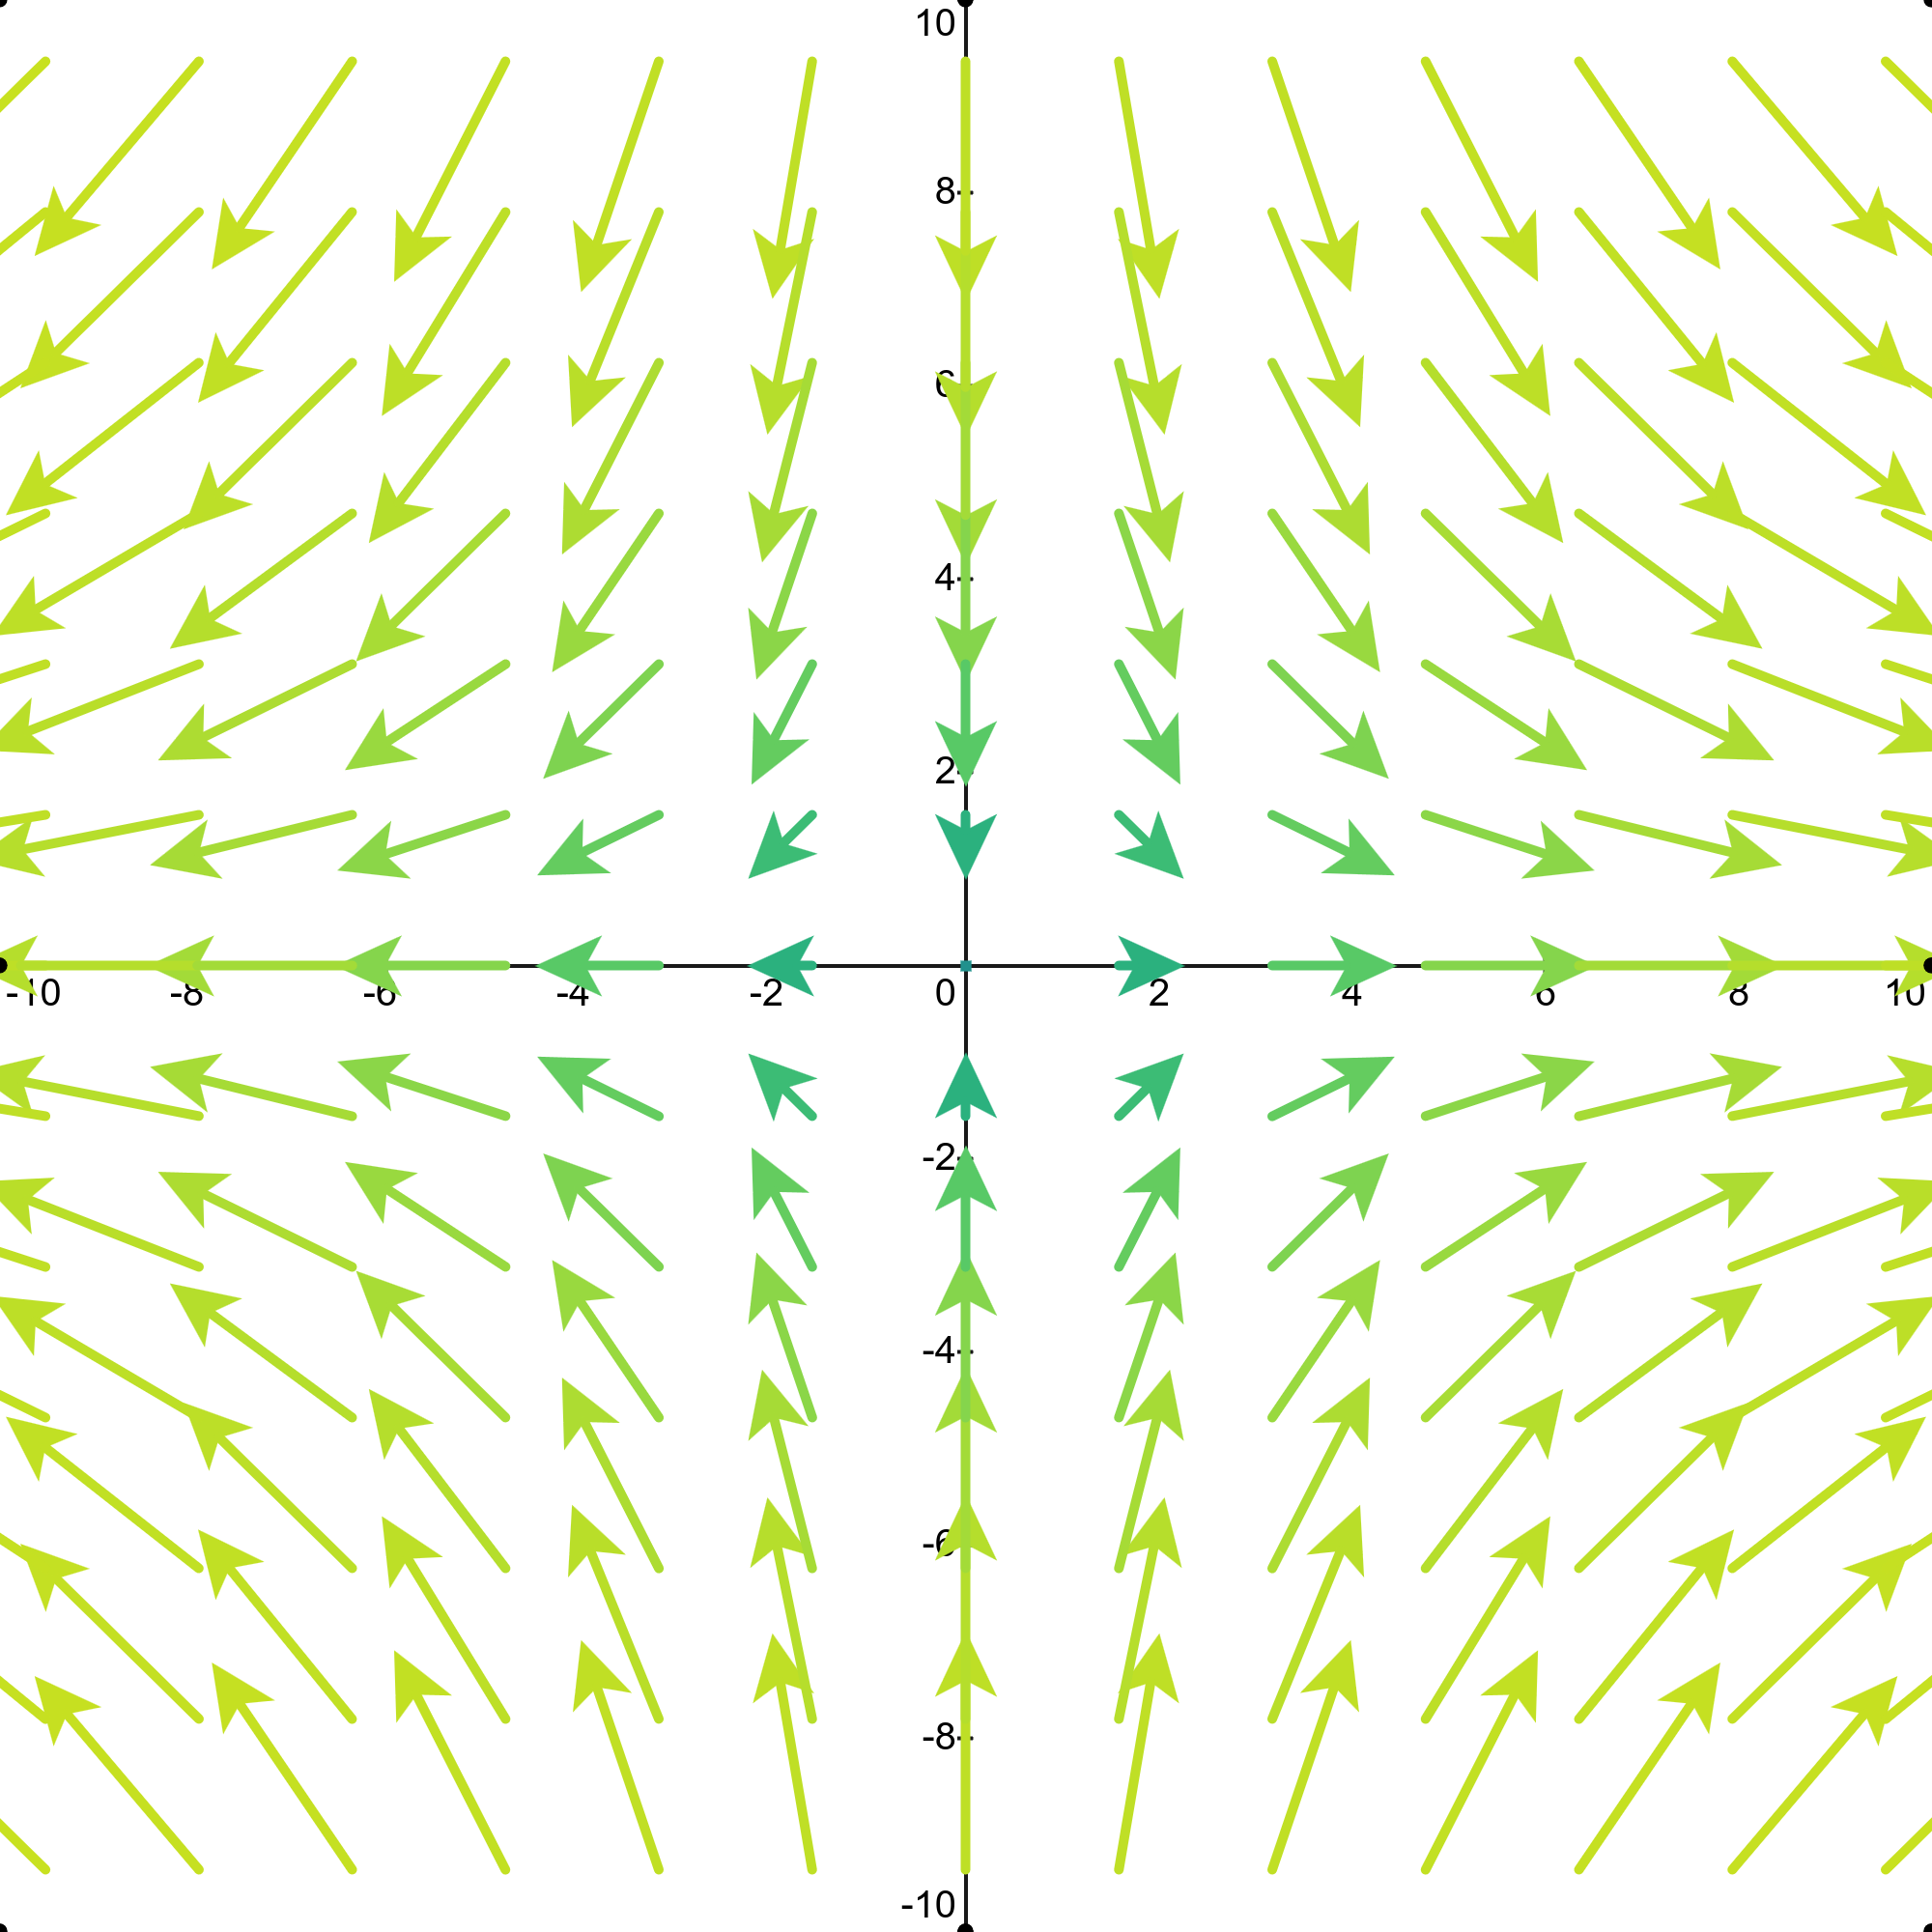
\includegraphics[width=1.7in]{slope-field-eig-pm-one-rot.png}
	\end{center}

	Both have eigenvalues $\pm 1$, but they have different eigenvectors.

	\begin{parts}
		\item How are the phase portraits related to each other?
		\item Suppose $P$ is a $2\times 2$ matrix with eigenvalues $\pm 1$. In what ways could
		the phase portrait for $\vec r'(t) = P\,\vec r(t)$ look \emph{different} from the above portraits?
		In what way(s) must it look the same?
	\end{parts}
\end{slide}

\begin{slide}
	\question
	\label{qclassifyorigin}
	Consider the following phase plane with lines in the direction of $\vec a$ (dashed green) and $\vec b$ (red).
			
			\begin{center}
			\begin{tikzpicture}[scale=1]
					\begin{axis}[
						width=5cm,
						height=5cm,
						xmin=-3.5,xmax=3.5,ymin=-3.5,
						ymax=3.5, xmajorgrids, ymajorgrids,
						xtick={-4,...,4}, ytick={-4,...,4}, axis lines=middle, yticklabels={,,}, xticklabels={,,},
						samples=5, domain=-5:5]
						
						\addplot[red, thick] {3*x} node[pos=0.6, left] {$\vec b$};
						\addplot[forestgreen, thick, dashed, dash pattern=on 3pt off 1pt] {1/3*x} node[pos=0.75, above] {$\vec a$};
					\end{axis}
			\end{tikzpicture}%
			\end{center}

	\begin{parts}
		\item Sketch a phase portrait where the directions $\vec a$ and $\vec b$ correspond to eigen solutions with eigenvalues that are

		\begin{tabular}{ccc}
		&sign for $\vec a$ & sign for $\vec b$\\
		\hline
		(1) & pos & pos\\
		(2) & neg & neg\\
		(3) & neg & pos\\
		(4) & pos & neg\\
		(5) & pos & zero\\
		\end{tabular}

		\item\label{partclassifyorigin} Classify the solution at the origin for situations (1)--(5) as stable or unstable.
		\item Would any of your classifications in \ref{qclassifyorigin}.\ref{partclassifyorigin} change if the directions of $\vec a$ and $\vec b$ changed?

	\end{parts}
\end{slide}


\begin{slide}
	\question
	You are examining a differential equation $\vec r'(t) = M\, \vec r(t)$ for an unknown $2\times 2$ matrix $M$.

	 You would like to determine whether $\vec r(t)=\mat{0\\0}$ is stable/unstable/attracting/repelling.
	\begin{parts}
		\item Come up with a rule to determine the nature of the equilibrium solution $\vec r(t) =\mat{0\\0}$ based on the eigenvalues of $M$ (provided there exists two linearly independent eigen solutions).
		\item Consider the system of differential equations
		\begin{align*}
			x'(t) &= x(t)+2\,y(t)\\
			y'(t) &= 3\, x(t)-4\,y(t)
		\end{align*}
		\begin{enumerate}
			\item Classify the stability of the equilibrium solution $(x(t), y(t))=(0,0)$ using any method you want.
			\item Justify your answer analytically using eigenvalues.
		\end{enumerate}
	\end{parts}
\end{slide}

%
% Hours 19-20
%

\begin{slide}
	\question
	Consider the following model of Social Media Usage where
	\begin{align*}
		P(t) &= \text{millions of social media posts at year $t$}\\
		U(t) &= \text{millions of social media users at year $t$}
	\end{align*}
	\begin{itemize}
		\item[(P1$_P$)] Ignoring all else, each year posts decay proportionally to the current number of posts with proportionality constant 1.
		\item[(P2$_P$)] Ignoring all else (independent of decay), posts grow by a constant amount of 2 million posts every year.
		\item[(P1$_U$)] Ignoring all else, social media users increase/decrease in proportion to the number of posts.
		\item[(P2$_U$)] Ignoring all else, social media users increase/decrease in proportion to the number of users.
		\item[(P3$_U$)] Ignoring all else, 1 million people stop using the platform every year.
	\end{itemize}

	\bigskip
	A school intervention is described by the parameter $a\in [-1/2, 1]$:
	\begin{itemize}
		\item After the intervention, the proportionality constant for (P1$_U$) is $1-a$.
		\item After the intervention, the proportionality constant for (P2$_U$) is $a$.
	\end{itemize}

	\begin{parts}
		\item Model this situation using a system of differential equations. Explain
			which parts of your model correspond to which premise(s).
	\end{parts}
\end{slide}

\begin{slide}
	\question
	The \textbf{SM} model of Social Media Usage is
	\begin{align*}
		P'&=-P+2\\
		U'&=(1-a)P + aU - 1
	\end{align*}
	where
	\begin{align*}
		P(t) &= \text{millions of social media posts at year $t$}\\
		U(t) &= \text{millions of social media users at year $t$}\\
		a &\in [-1/2, 1]
	\end{align*}

	\begin{parts}
		\item What are the equilibrium solution(s)?
		\item Make a phase portrait for the system.
		
		{\small \url{https://www.desmos.com/calculator/h3wtwjghv0}}
		\item Use phase portraits to conjecture: what do you think happens to the equilibrium
			solution(s) as $a$ transitions from negative to positive? Justify with a computation.
	\end{parts}
\end{slide}

\begin{slide}
	\question
	The \textbf{SM} model of Social Media Usage is
	\begin{align*}
		P'&=-P+2\\
		U'&=(1-a)P + aU - 1
	\end{align*}
	where
	\begin{align*}
		P(t) &= \text{millions of social media posts at year $t$}\\
		U(t) &= \text{millions of social media users at year $t$}\\
		a &\in [-1/2, 1]
	\end{align*}

	\begin{parts}
		\item Can you rewrite the system in matrix form? I.e., in the form $\vec r'(t) = M\, \vec r(t)$ for some matrix $M$ where $\vec r(t)=\Big(P(t), U(t)\Big)$.
		\item Define $\vec s(t)=\Big(S_P(t),S_U(t)\Big)$  to be the displacement from equilibrium in the \textbf{SM} model at time $t$ (provided an equilibrium exists).
		\begin{enumerate}
			\item Write $\vec s$ in terms of $P$ and $U$.
			\item Find $\vec s\,'$ in terms of $P$ and $U$.
			\item Find $\vec s\,'$ in terms of $S_P$ and $S_U$.
			\item Can one of your differential equation for $\vec s$ be written in matrix form? Which one?
			\item Analytically classify the equilibrium solution for your differential equation for $\vec s$
				when $a=-1/2$, $1/2$, and $1$. (You may use a calculator for computing eigenvectors/values.)
		\end{enumerate}
	\end{parts}
\end{slide}


\begin{slide}
	\question
	The \textbf{SM} model of Social Media Usage is
	\begin{align*}
		P'&=-P+2\\
		U'&=(1-a)P + aU - 1
	\end{align*}
	where
	\begin{align*}
		P(t) &= \text{millions of social media posts at year $t$}\\
		U(t) &= \text{millions of social media users at year $t$}\\
		a &\in [-1/2, 1]
	\end{align*}

	Some politicians have been looking at the model. They made the following posts on social media:
	\begin{enumerate}
			\item \emph{The model shows the number of posts will always be increasing. SAD!}
			\item \emph{I see the number of social media users always increases. That's not what we want!}
			\item \emph{It looks like social media is just a fad. Although users initially increase, they eventually settle down.}
			\item \emph{I have a dream! That one day there will be social media posts, but eventually there will be no social media users!}
	\end{enumerate}
		
	\begin{parts}
		\item For each social media post, make an educated guess about what initial conditions and what
		value(s) of $a$ the politician was considering.
		\item The school board wants to limit the number of social media users to fewer than 10 million.
		Make a recommendation about what value of $a$ they should target.
	\end{parts}
\end{slide}

%
% Hours 21-23
%


\begin{slide}
	\question
	Consider the following \textbf{FD} model of Fleas and Dogs where 
	\begin{align*}
		F(t) &= \text{number of parasites (fleas) at year $t$ (in millions)}\\
		D(t) &= \text{number of hosts (dogs) at year $t$ (in thousands)}
	\end{align*}
	\begin{itemize}
		\item[(P1$_F$)] Ignoring all else, the number of parasites decays in proportion to its population (with constant 1).
		\item[(P2$_F$)] Ignoring all else, parasite numbers grow in proportion to the number of hosts (with constant 1).
		\item[(P1$_D$)] Ignoring all else, hosts numbers grow in proportion to their current number (with constant 1).
		\item[(P2$_D$)] Ignoring all else, host numbers decrease in proportion to the number of parasites (with constant 2).
		\item[(P1$_c$)] Anti-flea collars remove 2 million fleas per year.
		\item[(P2$_c$)] Constant dog breeding adds 1 thousand dogs per year.
	\end{itemize}

	\bigskip
	\begin{parts}
		\item Write a system of differential equations for the \textbf{FD} model.
		\item Can you rewrite the system in matrix form $\vec r' = M\,\vec r$? What about in \emph{affine}
		form $\vec r' = M\,\vec r + \vec b$?
		\item Make a phase portrait for your model.
		\item What should solutions to the system look like in the phase plane? What are the equilibrium solution(s)?
	\end{parts}
\end{slide}


\begin{slide}
	\question
 		Recall the \textbf{FD} model of Fleas and Dogs where 
	\begin{align*}
		F(t) &= \text{number of parasites (fleas) at year $t$ (in millions)}\\
		D(t) &= \text{number of hosts (dogs) at year $t$ (in thousands)}\\
		\vec r(t) &= \mat{F(t)\\D(t)}
	\end{align*}
	and
	\[
		\vec r'(t) = \mat{-1&1\\-2&1}\,\vec r(t) + \mat{-2\\1}
	\]
	
	Define $\vec s(t)$ to be the displacement of $\vec r(t)$ from equilibrium at time $t$.
	\begin{parts}
		\item Find a formula for $\vec s$ in terms of $\vec r$.
		\item Can you find a matrix $M$ so that $\vec s'(t) = M\,\vec s(t)$?
		\item What are the eigenvalues of $M$?
		\item Find an eigenvector for each eigenvalue $M$?
		\item What are the eigen solutions for $\vec s'=M\,\vec s$?
	\end{parts}
\end{slide}

\begin{slide}
	\question
 		Recall the \textbf{FD} model of Fleas and Dogs where 
	\begin{align*}
		F(t) &= \text{number of parasites (fleas) at year $t$ (in millions)}\\
		D(t) &= \text{number of hosts (dogs) at year $t$ (in thousands)}\\
		\vec r(t) &= \mat{F(t)\\D(t)} \qquad\qquad
		\vec s(t) = \vec r(t) - \mat{3\\5}
	\end{align*}
	and
	\begin{align*}
		\vec s\,'(t) &= M\,\vec s(t)\qquad\text{where}\qquad M=\mat{-1&1\\-2&1}.
	\end{align*}
	
	This equation has eigen solutions
	\begin{align*}
		\vec s_1(t) &= e^{it}\matc{1-i\\2}\\
		\vec s_2(t) &= e^{-it}\matc{1+i\\2}
	\end{align*}
	
	\begin{parts}
		\item Recall Euler's formula $e^{it}=\cos(t)+i\sin(t)$. 
		\begin{enumerate}
			\item Use Euler's formula to expand $\vec s_1 + \vec s_2$. Are there any imaginary numbers remaining?
			\item Use Euler's formula to expand $i(\vec s_1 - \vec s_2)$. Are there any imaginary numbers remaining?
		\end{enumerate}
		\item Verify that your formulas for $\vec s_1+\vec s_2$ and $i(\vec s_1-\vec s_2)$ are solutions to
			$\vec s\,'(t) = M\,\vec s(t)$.
		\item Can you give a third \emph{real} solution to $\vec s\,'(t) = M\,\vec s(t)$?
	\end{parts}
\end{slide}

\begin{slide}
	\question
 		Recall the \textbf{FD} model of Fleas and Dogs where 
	\begin{align*}
		F(t) &= \text{number of parasites (fleas) at year $t$ (in millions)}\\
		D(t) &= \text{number of hosts (dogs) at year $t$ (in thousands)}\\
		\vec r(t) &= \mat{F(t)\\D(t)} \qquad\qquad
		\vec s(t) = \vec r(t) - \mat{3\\5}
	\end{align*}
	and
	\begin{align*}
		\vec s\,'(t) &= M\,\vec s(t)\qquad\text{where}\qquad M=\mat{-1&1\\-2&1}.
	\end{align*}
	
	\begin{parts}
		\item What is the dimension of the space of solutions to $\vec s\,'(t) = M\,\vec s(t)$?
		\item Give a basis for all solutions to $\vec s\,'(t) = M\,\vec s(t)$.
		\item Find a solution satisfying $\vec s(0)=\mat{1\\3}$.
		\bigskip 
		\item Using what you know, find a general formula for $\vec r(t)$.
		\item Find a formula for $\vec r(t)$ satisfying $\vec r(0)=\mat{4\\8}$.
	\end{parts}
\end{slide}


\begin{slide}
	\question
 		Recall the \textbf{FD} model of Fleas and Dogs where 
	\begin{align*}
		F(t) &= \text{number of parasites (fleas) at year $t$ (in millions)}\\
		D(t) &= \text{number of hosts (dogs) at year $t$ (in thousands)}\\
		\vec r(t) &= \mat{F(t)\\D(t)} \qquad\qquad
		\vec s(t) = \vec r(t) - \mat{3\\5}
	\end{align*}
	and
	\begin{align*}
		\vec s\,'(t) &= M\,\vec s(t)\qquad\text{where}\qquad M=\mat{-1&1\\-2&1}.
	\end{align*}

	Some research is being done on a shampoo for the dogs. It affects flea and dog reproduction:
	\begin{itemize}
		\item[(PS$_F$)] Ignoring all else, the number of parasites decays in proportion to its population with constant $1+a$.
		\item[(PS$_D$)] Ignoring all else, hosts numbers grow in proportion to their current number with constant $1-a$.
	\end{itemize}
	
	\vspace{-1.5em}
	where $-1\leq a\leq 1$. \emph{These premises replace (P1$_F$) and (P1$_D$).}
	
	\begin{parts}
		\item Modify the previous \textbf{FD} model to incorporate the effects of the shampoo.
		\item Make a phase portrait for the \textbf{FD Shampoo} model.
		\item Find the equilibrium solutions for the \textbf{FD Shampoo} model.
		\item For each equilibrium solution determine its stability/instability/etc..
		\item Analytically justify your conclusions about stability/instability/etc..
	\end{parts}
\end{slide}

\begin{slide}
	\question
		Consider the differential equation
		\[
		\vec s\,'(t) = M\vec s(t)\qquad\text{where}\qquad M=\mat{-1&-4\\2&3}
		\]
	
	\begin{parts}
		\item Make a phase portrait. Based on your phase portrait, classify the equilibrium solution.

		{\small \url{https://www.desmos.com/calculator/h3wtwjghv0}}
		\item Find eigen solutions for this differential equation (you may use a calculator/computer to assist).
		\item Find a general \emph{real} solution.
		\item Analytically classify the equilibrium solution.
	\end{parts}
\end{slide}


%
% Hours 24-26
%


\begin{slide}
	%
	% Completed phase portrait in desmos:
	% https://www.desmos.com/calculator/tvjag852ja
	\question
	Recall the tree model from Question \ref{q-phase}:
	\begin{itemize}
		\item $H(t)\ =$ height (in meters) of tree trunk at time $t$
		\item $A(t)\ =$ surface area (in square meters) of all leaves at time $t$
	\end{itemize}
	\begin{align*}
		H'(t) &= 0.3\cdot A(t)-b\cdot H(t)\\
		A'(t) &= -0.3\cdot (H(t))^2 + A(t)
	\end{align*}
	and $0 \leq b \leq 2$

	A phase portrait for this model is available at 
	
		{\small
		\url{https://www.desmos.com/calculator/tvjag852ja}
		}
	\bigskip
	\phantom{x}
	\begin{parts}
		\item Visually classify the nature of each equilibrium solution as attracting/repelling/etc.. 
		Does the nature depend on $b$? Are you confident in your visual assessment?
		\item Can you rewrite the system in matrix/affine form? Why or why not?
	\end{parts}
	\bigskip
	\phantom{x}
\end{slide}

\begin{slide}
	\question\label{qapprox1d}
	A simple logistic model for a population is
	\[
		\frac{\d P}{\d t} = P(t)\cdot\left(1-\frac{P(t)}{2}\right)
	\]
	where $P(t)$ represents the population at time $t$.
	
	We'd like to approximate $\d P/\d t$ when $P\approx 1/2$.
	\begin{parts}
		\item What is the value of $\d P/\d t$ when $P=1/2$?
		
		\item %\hbox{\vbox{
			Define $f(P)=P(t)\cdot\left(1-\frac{P(t)}{2}\right)$ and notice\\ $\d P/\d t = f(P)$.

		Approximate $\d P/\d t$ (i.e, approximate $f$) when\\ $P=1/2+\Delta$ and $\Delta$ is small.
		%}}

		\bigskip
		\item Write down an approximation $S(\Delta)$ that approximates $\d P/\d t$ when $P$ is $\Delta$ away from $1/2$.
		\item 
		
		Let $A_{1/2}(P)$ be an \emph{affine} approximation to $\d P/\d t$ that is a good approximation when $P\approx 1/2$.
		Find a formula for $A_{1/2}(P)$.
		\item Find additional affine approximations to $\d P/\d t$ centered at each equilibrium solution.
		\vspace{1cm}
		\phantom{x}
	\end{parts}
\end{slide}

\begin{slide}
	\question
	Based on our calculations from Exercise \ref{qapprox1d}, we have several different affine approximations.

	\begin{tabular}{rll}
		(Original) & $P'=P(1-P/2)$
		& ({\small \url{https://www.desmos.com/calculator/v1coz4shtw}})\\
		($A_{1/2}$) & $P'\approx \frac{3}{8}+\frac{1}{2}(P-\frac{1}{2})$
		& ({\small \url{https://www.desmos.com/calculator/zsb2apxhqs}})\\
		($A_0$) & $P'\approx P$
		& ({\small \url{https://www.desmos.com/calculator/vw48bvqgrc}})\\
		($A_2$) & $P'\approx -(P-2)$
		& ({\small \url{https://www.desmos.com/calculator/i2utk6vnqh}})\\

	\end{tabular}
	
	\begin{parts}
		\item What are the similarities/differences in the Desmos plots of solutions
		to the original equation vs. the other equations?
		\item Does the nature of the equilibrium solutions change when using an affine approximation?
		\item Classify each equilibrium solution of the original equation by using affine approximations.
	\end{parts}
\end{slide}

\begin{slide}
	\question
	Consider the differential equation whose slope field is sketched below.
	\begin{align*}
		P'(t) &= -P(t)\cdot(0.1+P(t))\cdot(0.2+P(t))\\ 
		&=-(P(t))^3-0.3\cdot (P(t))^2 -0.02\cdot P(t)
	\end{align*}

	{\small \url{https://www.desmos.com/calculator/ikp9rgo0kv}}
	\begin{center}
	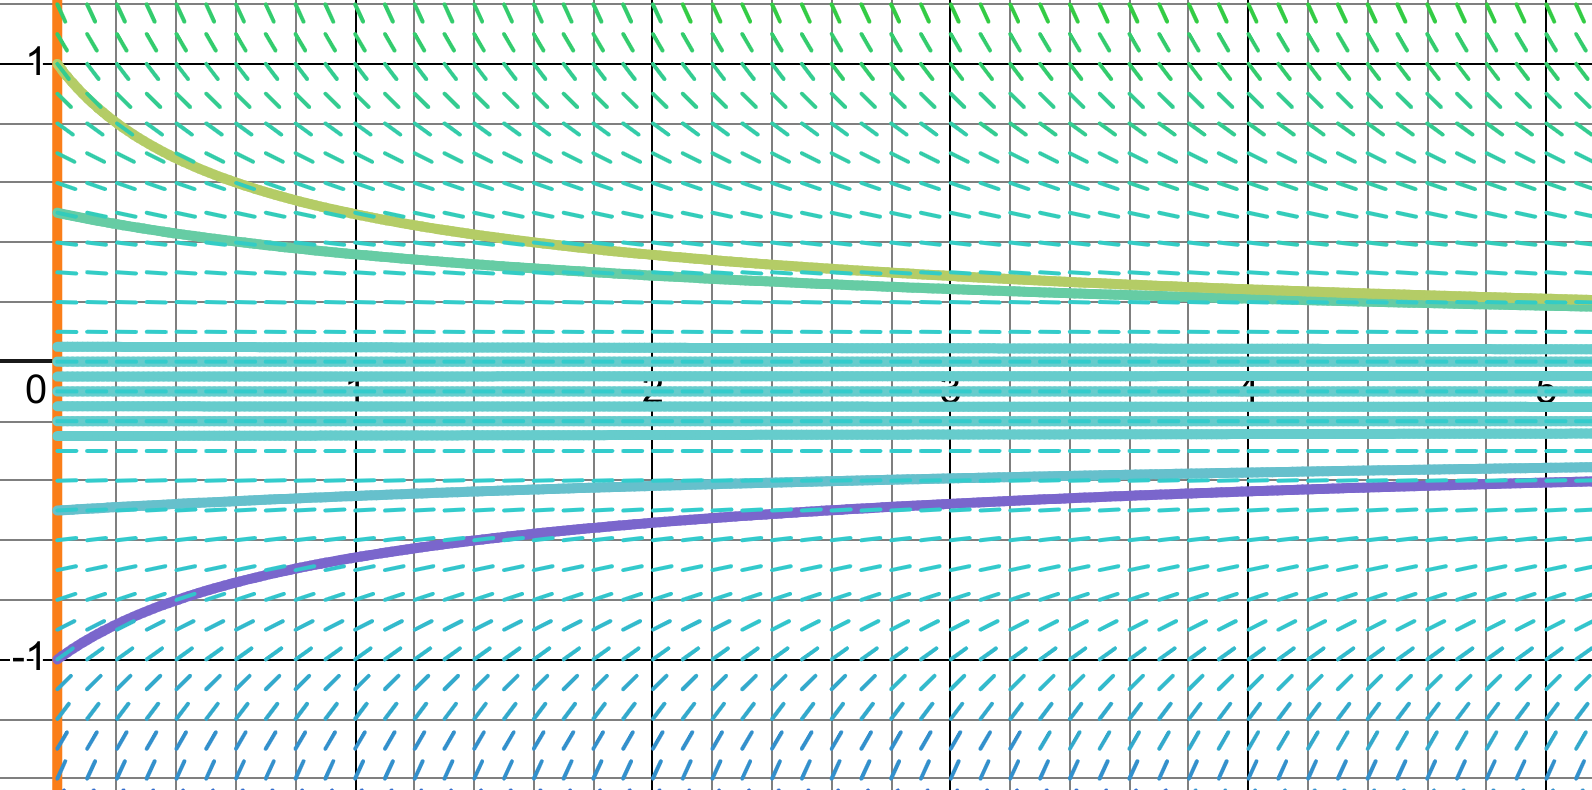
\includegraphics[width=2.5in]{slope-field-ambiguous.png}
	\end{center}


	\bigskip	
	\bigskip	
	\bigskip	
	\begin{parts}
		\item Find all equilibrium solutions.
		\item Use affine approximations to classify the equilibrium solutions as stable/unstable/etc..
	\end{parts}
\end{slide}

\begin{slide}
	\question
	To make a 1d affine approximation of a function $f$ at the point $E$ we have the formula
	\[
		f(x)\qquad \approx\qquad f(E) + f'(E)(x-E).
	\]		

	To make a 2d approximation of a function $\vec F(x,y)=\Big(F_1(x,y), F_2(x,y)\Big)$ at the point $\vec E$,
	we have a similar formula
	\[
		\vec F(x,y)\qquad \approx \qquad \vec F(\vec E) + D_{\vec F}(\vec E)\left(\mat{x\\y}-\vec E\right)
	\]
	where $D_{\vec F}(\vec E)$ is the \emph{total derivative} of $\vec F$ at $\vec E$, which can be expressed
	as the matrix
	\[
		D_{\vec F}(\vec E) = \mat{
			\rule[-0.5cm]{0pt}{.8cm}\displaystyle \frac{\partial F_1}{\partial x} &\displaystyle  \frac{\partial F_1}{\partial y}\\
			\rule[-0.2cm]{0pt}{.3cm}\displaystyle  \frac{\partial F_2}{\partial x} &\displaystyle  \frac{\partial F_2}{\partial y}
		}
	\]
	evaluated at $\vec E$.
\end{slide}

\begin{slide}

	Recall our model from Exercise \ref{q-phase} for the life cycle of a tree where $H(t)$ was
	height, $A(t)$ was the leaves' surface area, and $t$ was time:
	\begin{align*}
		H'(t) &= 0.3\cdot A(t)-b\cdot H(t)\\
		A'(t) &= -0.3\cdot (H(t))^2 + A(t)
	\end{align*}
	with $0 \leq b \leq 2$

	\bigskip
	
	We know the following:
	\begin{itemize}
		\item The equations cannot be written in matrix form.
		\item The equilibrium points are $(0,0)$ and $\Big(\frac{100}{9}b,\frac{1000}{27}b^2\Big)$.			
	\end{itemize}	

	We want to find an affine approximation to the system.

	Define $\vec F(H,A)=(H', A')$
	\begin{parts}
		\item Find the matrix for $D_{\vec F}$, the total derivative of $\vec F$.
		\item Create an affine approximation to $\vec F$ around $\vec e=(0,0)$ and use this to write an approximation to the original system.
		\item In the original system, the equilibrium $(0,0)$ is unstable and not repelling. Justify this using your affine approximation.
		\item\label{affine-approx}
		 Create an affine approximation to $\vec F$ around $\vec e=(\frac{100}{9}b,\frac{1000}{27}b^2)$ and use this to write an approximation to the original system.
		
		\item Make a phase portrait for the original system and your approximation from part \ref{affine-approx}. How do they compare?
		\item Analyze the nature of the equilibrium solution in part \ref{affine-approx} using eigen techniques. Relate your analysis to
		the original system.

	\end{parts}
\end{slide}


\begin{slide}
	\question
	Define $\vec F(x,y)=\matc{y\\-xy+x^2-x-y}$ and consider the differential equation
	\[
		\mat{x'\\y'}=\vec F(x,y).
	\]



	\begin{parts}
		\item Make a phase portrait for this differential equation. Based on your phase 
		portrait, can you determine the nature of the equilibrium at $(0,0)$?

		{\small \url{https://www.desmos.com/calculator/peby3xd7jj}}

		\bigskip
		\item Find an affine approximation to $\vec F$ centered at $(0,0)$.
		\item Write down a differential equation that approximates the original equation 
		near $(0,0)$.
		\item Analyze the nature of the equilibrium solution $\vec r(t)=(0,0)$ using eigen techniques. (You may use a computer to assist in eigen computations.) Relate your analysis to
		the original system.

		\bigskip
		\phantom{x}
	\end{parts}
\end{slide}

%
% Hours 27-29
%

\begin{slide}
	\question
	Consider a spring with a mass attached to the end.
	
	\begin{tikzpicture}[scale=.4]
		\draw[ultra thick] (0,-1) -- (0,1);
		\draw[ultra thick,variable=\t,domain=1.5:30,samples=150] plot ({0.6+1.2*(0.3*\t-sin(180*\t/pi))},{1.2*(1-cos(180*\t/pi))-1});
		\draw[fill=brown!65!black,draw=none] (-1,-1) rectangle (0,1);
		\draw[fill=gray!50!white,ultra thick] ({0.6+1.2*(0.3*30-sin(180*30/pi))},{1.2*(1-cos(180*30/pi))-1}) circle (1) node {M};
	\end{tikzpicture}
	%[XXX Diagram] |-www-[M]
	
	Let $x(t) =$ displacement to the right of the spring from equilibrium at time $t$
	
	Recall from Physics the following laws:
	\vspace{-1em}
	\begin{itemize}
		\item[(HL)] Hooke's Law: For an elastic spring, force is proportional to negative the displacement from equilibrium. 
		\item[(NL)] Newton's Second Law: Force is proportional to acceleration (the proportionality constant is called \emph{mass}).
		\item[(ML)] Laws of Motion: Velocity is the time derivative of displacement and acceleration is the time derivative of velocity.
	\end{itemize}

	\bigskip
	\bigskip
	\begin{parts}
		\item Model $x(t)$ with a differential equation.
		
		For the remaining parts, assume the elasticity of the spring is $k=1$ and the mass is $1$.
		\item Suppose the spring is stretched $0.5m$ from
		equilibrium and then let go (at time $t=0$).
		\begin{enumerate}
			\item At $t=0$, what are $x$, $x'$, and $x''$?
			\item Modify Euler's method to approximate a solution to the initial value problem.
		\end{enumerate}

		\item Introduce the auxiliary equation $y=x'$. Can the second-order spring equation
		be rewritten as a first-order system involving $x'$ and $y'$? If so, do it.
		
		\item Simulate the system you found in the previous part using Euler's method.
		
	\end{parts}
	\bigskip
	\phantom{x}
\end{slide}

\begin{slide}
	\question
	Recall the a spring with a mass attached to the end.
	
	\begin{tikzpicture}[scale=.4]
		\draw[ultra thick] (0,-1) -- (0,1);
		\draw[ultra thick,variable=\t,domain=1.5:30,samples=150] plot ({0.6+1.2*(0.3*\t-sin(180*\t/pi))},{1.2*(1-cos(180*\t/pi))-1});
		\draw[fill=brown!65!black,draw=none] (-1,-1) rectangle (0,1);
		\draw[fill=gray!50!white,ultra thick] ({0.6+1.2*(0.3*30-sin(180*30/pi))},{1.2*(1-cos(180*30/pi))-1}) circle (1) node {M};
	\end{tikzpicture}
	
	$x(t) =$ displacement to the right of the spring from equilibrium at time $t$
	
	
	We have two competing models
	\begin{equation}
		x''=-kx \tag{A}
	\end{equation}
	\vbox{% prevent the equation and its description from splitting across columns
	\begin{equation}
			\mat{x\\y}' = \mat{0&1\\-k&0}\mat{x\\y}
		\tag{B}
	\end{equation}
	where $y=x'$.
	}

	\bigskip
	\begin{parts}
		\item Make a phase portrait for system (B). What are the axes on the phase portrait? What do you expect general solutions to look like?
		\item Use eigenvalues/eigenvectors to find a general solution to (B). (You may use a computer to compute eigenvalues/vectors.)
		\item Use your solution to (B) to find a general solution to (A).
		
	\end{parts}
\end{slide}

\begin{slide}
	\question
	Consider the second-order differential equation
	\[
		x''=-(1+x)\cdot x'+x^2-x
	\]

	\begin{parts}
		\item Rewrite the second-order differential equation as a system of first-order differential equations. (Hint:
		you may need to introduce an auxiliary equation.)

		\item The following Desmos link plots a phase portrait and draws an Euler approximation on the phase portrait:

		{\small \url{https://www.desmos.com/calculator/fvqxqp6eds}}

		Use the link to make a phase portrait for your system and answer the following questions:
		\begin{enumerate}
			\item Are there initial conditions with $x(0)<0$ so that a solution $x(t)$ is always increasing?
			\item Are there initial conditions with $x(0)<0$ so that a solution $x(t)$ first decreases and then increases?
		\end{enumerate}

		\item Show that $x(t)=0$ is an equilibrium solution for this equation.

		\item Use linearization and eigenvalues to classify the equilibrium $(x,x')=(0,0)$
		in phase space.

		\item Let $x(t)$ be a solution to the original equation and suppose $x(0)=\delta_1\approx 0$.
		\begin{enumerate}
			\item If $x'(0)=\delta_2\approx 0$, speculate on the long term behaviour of $x(t)$.
			\item If we put no conditions on $x'(0)$ will your answer be the same? Explain.
		\end{enumerate}

	\end{parts}
\end{slide}

\begin{slide}
	\textbf{Boundary Value Problems}

	\question
	Recall the spring-mass system modeled by
	\[
		x''=-x
	\]
	We would like to use the spring-mass system to ring a bell at regular intervals, 
	so we put a hammer at the end of the spring. Whenever the displacement is maximal,
	the hammer strikes a bell producing a ring.

	\begin{parts}
		\item Convert the spring-mass system into a system of differential equations.
		Make a phase portrait for the system using the following Desmos link:

		{\small \url{https://www.desmos.com/calculator/fvqxqp6eds}}
		\item In the \emph{Options Euler} on Desmos, adjust $\Delta$ and the number of steps so that simulated solutions are only 
		shown for $t\in[0,1]$.

		Use simulations to answer the remaining questions.
		\item You start by displacing the hammer by $1m$ and letting go. Is it possible that the bell rings every 1 second?
		\item You start by displacing the hammer by $1m$ and giving the hammer a push. Is it possible that the bell rings every 1 second?
		\item What is the smallest amount of time between consecutive rings (given a positive displacement)?
	\end{parts}
\end{slide}

\begin{slide}
	\textbf{Boundary Value Problems}

	\question
	Recall the spring-mass system modeled by
	\[
		x''=-x
	\]
	We would like to use the spring-mass system to ring a bell at regular intervals, 
	so we put a hammer at the end of the spring. Whenever the displacement is maximal,
	the hammer strikes a bell producing a ring.

	Consider the subspaces
	\[
		S_1=\Span\{\,\sin(t),\cos(t)\,\}\quad S_2=\{\,A\cos(t+d):A,d\in\R\,\}
	\]

	\begin{parts}
		\item What dimension is each subspace?
		\item Which subspaces are sets of solutions to the spring-mass system?
		\item Use what you know about complete solutions and linear algebra to prove $S_1=S_2$.

		\medskip
		Use your knowledge about $S_1$ and $S_2$ to analytically answer the remaining questions.
		\item You start by displacing the hammer by $1m$ and letting go. Is it possible that the bell rings every 1 second?
		\item You start by displacing the hammer by $1m$ and giving the hammer a push. Is it possible that the bell rings every 1 second?
		\item What is the smallest amount of time between consecutive rings (given a positive displacement)?
	\end{parts}
\end{slide}

\begin{slide}
	\textbf{Boundary Value Problems}

	\question
		A \emph{boundary value problem} is a differential equation paired with two conditions
		at different values of $t$.

		Consider the following boundary value problems:
		\begin{center}
			\begin{tabular}{ccc}
				(i) & (ii) & (iii) \\
				$x''=-x$ &
				$x''=-x$ &
				$x''=-x$ \\
				$x(0)=1$ &
				$x(0)=1$ &
				$x(0)=1$ \\ 
				$x(\pi)=1$ & 
				$x(\pi)=-1$ & 
				$x(\frac{\pi}{2})=0$
			\end{tabular}
		\end{center}

	\begin{parts}
		\item Using phase portraits and simulations, determine how many solutions each boundary value problem has.
		\item Can you find analytic arguments to justify your conclusions?

	\end{parts}
\end{slide}

\begin{slide}
	\textbf{Existence and Uniqueness}

	Whether a solution to a differential equations exists or is unique is a \emph{hard} question
	with many partial answers.

	\begin{theorem}[Existence and Uniqueness II]
		Let $F(t,x,x')=0$ with $x(t_0)=x_0$ describe an initial value problem.

		~~\hbox{\vbox{
		\begin{itemize}
		\item[IF] $F(t,x,x')=x'(t)+p(t)x(t)+g(t)$ for some functions $p$ and $g$\quad 
		\item[AND]
		$p$ and $g$ are continuous on an open interval $I$ containing $t_0$\quad 
		\item[THEN]
		the initial value problem has a unique solution on $I$.
		\end{itemize}
		}}
	\end{theorem}

	\question

	\begin{parts}
		\item The theorem expresses differential equations in the form $F(t,x,x',x'',\ldots)=0$ 
		(i.e. as a level set of some function $F$).

		Rewrite the following differential equations in the form $F(t,x,x',x'',\ldots)=0$:\\
			(i) $x''=-kx$\qquad
			(ii) $x''=-x\cdot x'+x^2$\quad\\
			(iii) $x'''=(x')^2-\cos x$

		\item Which of the following does the theorem say \emph{must} have a unique solution on 
		an interval containing $0$?
		\begin{enumerate}
			\item $y'=\frac{3}{2}y^{1/3}$ with $y(0)=0$
			\item $x'(t)=\lfloor t\rfloor x(t)$ with $x(0)=0$
			\item $x'(t)=\lfloor t-\frac{1}{2}\rfloor x(t)+t^2$ with $x(0)=0$
		\end{enumerate}

		Note: $\lfloor x\rfloor$ is the \emph{floor} of $x$, i.e., the largest integer less than or equal to $x$.

	\end{parts}
\end{slide}




\begin{slide}

\question

Consider a rope hanging from two poles.

\vspace{-1em}
\begin{center}
%\begin{tikzpicture}
%  \draw (-1,0) node[below] {0} -- (-1,{cosh(-1)});
%  \draw (1.5,0) node[below] {1} -- (1.5,{cosh(1.5)});
%  \draw[fill=brown!65!black,draw=none] (-1.5,-0.1) rectangle (2,0);
%  \draw (-1.5,0) -- (2,0);
%  \draw[blue, ultra thick, variable=\x,domain=-1:1.5,samples=100] plot ({\x},{cosh(\x)});
%\end{tikzpicture}	
\begin{tikzpicture}
  \draw (-1,0) -- (-1,{cosh(-1)});
  \draw (1.5,0) -- (1.5,{cosh(1.5)});
  \draw[fill=brown!65!black,draw=none] (-1.5,-0.1) rectangle (2,0);
  \draw (-1.5,0) -- (2,0);
  \draw[blue, thick, variable=\x,domain=-1:1.5,samples=100] plot ({\x},{cosh(\x)});
  \draw[ultra thick,violet!50!white] (0,1) -- (0.5,{cosh(0.5)});
  \draw[->] (0,1) -- node[above] {\small $\vec{T}_L$} (-0.5,{2-cosh(0.5)+0.15});
  \draw[->] (0.5,{cosh(0.5)}) -- node[above] {\small $\vec{T}_R$} (1,{2*cosh(0.5)-1+0.15});
  \draw[->] (0.25,0.9) -- (0.25, 0.5) node[below] {\small $\vec{F}_g$};
  \draw[dashed,gray] (0,-0.12) node[below] {\scriptsize $d$} -- (0,1);
  \draw[dashed,gray] (0.5,-0.12) node[below] {\scriptsize $\quad d+\Delta$} -- (0.5,{cosh(0.5)});
\end{tikzpicture}
\end{center}
\vspace{-1em}
$H(d)=$ height of the rope above ground at position $d$.

We will consider the following premises and physics laws:
\vspace{-1em}
\begin{itemize}
	\item[($P_D$)] The linear density of the rope is constant: $\rho$ kg/m

	\item[($P_G$)] Gravity pulls downwards in proportion to mass (the proportionality constant is called $g$)
	
	\item[($P_T$)] Tension pulls tangentially to the rope

%	\item[(S)] The rope is not moving (it is stationary)

	\item[($P_{NL}$)] Newton's First Law: a body at rest will remain at rest unless it is acted upon by a force

%	\item[(NL)] Newton's Second Law: Force is proportional to acceleration (the proportionality constant is called mass).

%	\item[(ML)] Laws of Motion: Velocity is the time derivative of displacement and acceleration is the time derivative of velocity.
\end{itemize}

To model the rope, imagine it is made of \textbf{small rigid rods}.
We will focus on one such rod, $S$, (drawn in the figure) from $d$ to $d+\Delta$.

\begin{parts}

\item Given ($P_{NL}$), find a relation between the force vectors $\vec{T}_L, \vec{T}_R, \vec{F}_g$.
\item Approximate the length of the segment $S$ and its mass. Approximate the vector $\vec{F}_g$.
\item Find a vector $\vec{V}_L$ in the direction of $\vec{T}_L$ (the magnitude doesn't matter at this point).
\end{parts}
	
\end{slide}


\begin{slide}

\question

Consider a rope hanging from two poles.

The only forces acting on the rope are gravity and tension.
\vspace{-1em}
\begin{center}
%\begin{tikzpicture}
%  \draw (-1,0) node[below] {0} -- (-1,{cosh(-1)});
%  \draw (1.5,0) node[below] {1} -- (1.5,{cosh(1.5)});
%  \draw[fill=brown!65!black,draw=none] (-1.5,-0.1) rectangle (2,0);
%  \draw (-1.5,0) -- (2,0);
%  \draw[blue, ultra thick, variable=\x,domain=-1:1.5,samples=100] plot ({\x},{cosh(\x)});
%\end{tikzpicture}	
\begin{tikzpicture}
  \draw (-1,0)  -- (-1,{cosh(-1)});
  \draw (1.5,0)  -- (1.5,{cosh(1.5)});
  \draw[fill=brown!65!black,draw=none] (-1.5,-0.1) rectangle (2,0);
  \draw (-1.5,0) -- (2,0);
  \draw[blue, thick, variable=\x,domain=-1:1.5,samples=100] plot ({\x},{cosh(\x)});
  \draw[ultra thick,violet!50!white] (0,1) -- (0.5,{cosh(0.5)});
  \draw[->] (0,1) -- node[above] {\small $\vec{T}_L$} (-0.5,{2-cosh(0.5)+0.15});
  \draw[->] (0.5,{cosh(0.5)}) -- node[above] {\small $\vec{T}_R$} (1,{2*cosh(0.5)-1+0.15});
  \draw[->] (0.25,0.9) -- (0.25, 0.5) node[below] {\small $\vec{F}_g$};
  \draw[dashed,gray] (0,-0.12) node[below] {\scriptsize $d$} -- (0,1);
  \draw[dashed,gray] (0.5,-0.12) node[below] {\scriptsize $\quad d+\Delta$} -- (0.5,{cosh(0.5)});
\end{tikzpicture}
\end{center}
\vspace{-1em}


Similarly to the previous exercise, we can find a vector $\vec{V}_R = \matc{1\\H'(d+\Delta)}$ in the direction of $\vec{T}_R$, but with possibly different magnitude.

So far we have:
\begin{itemize}
	\item $\vec{T}_L = \alpha \vec{V}_L$  for some $\alpha > 0$, and
	\item $\vec{T}_R = \beta \vec{V}_R$ for some $\beta >0$.
\end{itemize}


\begin{parts}

\item Can you find approximations of the vectors $\vec{F}_g, \vec{T}_L, \vec{T}_R$ that only use $H(d)$, $H'(d)$, and $H''(d)$?

Hint:
	\begin{itemize}
		\item $H(d+\Delta) \approx H(d) + \Delta \cdot H'(d)$,
		\item $H'(d+\Delta) \approx H'(d) + \Delta \cdot H''(d)$.
	\end{itemize}

\item Put everything together to find a (second order) differential equation for $H$.

\item Do $\alpha$ or $\beta$ depend on $d$? Explain.
	
\end{parts}
		
\end{slide}


\begin{slide}

\question

Recall a rope hanging from two poles.

\vspace{-1em}
\begin{center}
\begin{tikzpicture}
  \draw (-1.5,0)  -- (-1.5,{cosh(-1.5)});
  \draw (1.5,0) -- (1.5,{cosh(1.5)});
  \draw[fill=brown!65!black,draw=none] (-2,-0.1) rectangle (2,0);
  \draw (-1.5,0) -- (2,0);
  \draw[blue, ultra thick, variable=\x,domain=-1.5:1.5,samples=100] plot ({\x},{cosh(\x)});
\end{tikzpicture}
\end{center}
\vspace{-1em}
$H(d)=$ the height of the rope at position $d$.

We have the following model for it:
\[
H''(d) = k \sqrt{1+\big(H'(d)\big)^2}
\]
\vspace{1pt}

Toronto Hydro is stringing some wire. The posts are 20m apart and at a height of 10m. At the lowest point, the wire is 5m above the ground.
\begin{parts}

	\item Set up a boundary value problem that can be used to find the total length of the wire.

	\item Using the following Desmos link, can you find a solution to the boundary value problem?

		{\small \url{https://www.desmos.com/calculator/l4fair6454}}

	
	\item It happens that $k=\frac{\rho g}{T}$ where $T$ is the minimum tension in the rope.

	Suppose Toronto Hydro hung the wires so that they were at minimum 9m above the ground.
	Would the tension be higher or lower? By how much?

	\item Should the difference between maximum and minimum tension
	be higher or lower for low-hanging wires? What does your intuition say? What does the phase portrait say?

	%The wire has a (linear) density of 1 kg/m and gravity is 9.8 m/s$^2$.
	
	%For safety reasons, the wire's tensile strength needs to be 5 times the maximum tension when the wire is resting.
	
	%What strength of wire do they need?
	
	%\item Assuming the posts are both the same height, relate the length of the rope with the tension at the posts. 

	%\item Assuming the posts have different heights, relate the length of the rope with the tension at the posts. 
	
\end{parts}


	
\end{slide}





\begin{bookonly}
%\begin{appendix}\label{APPSLEI}
%	\Title{Systems of Linear Equations I}
%
%	In this appendix you will learn
%	\begin{itemize}
%		\item What a system of linear equations is.
%		\item What the solution set to a system of equations is, and what it means for a system of equations
%			to be consistent or inconsistent.
%		\item How augmented matrices can be used to solve systems of linear equations.
%		\item How to apply row reduction to find a unique solution to a system of linear
%			equations and to determine if a system of linear equations is consistent or inconsistent.
%	\end{itemize}
%
%		An \emph{equation} encodes a relationship between quantities. For
	example, writing
	\[
		\underbrace{\text{Slices of cake}}_C = \underbrace{\text{Slices you ate}}_M + \underbrace{\text{Slices your brother ate}}_B
	\]
	specifies a precise relationship between the quantities $C$, $M$, and $B$. 
	Without more information, $C$, $M$, and $B$ could be almost anything. As such, we call 
	$C$, $M$, and $B$
	\emph{variables} or \emph{unknowns}. 
	However, the
	relationship \emph{between} them is precisely defined. 

	Additional relationships give rise to additional equations, which we express concisely as a
	\emph{system of equations}, that is, a list of equations. For example, suppose you know the cake
	had six pieces and your brother ate twice as many pieces as you. We might now write the system
 
	\begin{align*}
  		C &= M + B \\
  		B &= 2M \\
  		C &= 6
	\end{align*}
 
	which should be interpreted as: ``the relationship $C=M+B$ holds \emph{and} the relationship $B=2M$ holds \emph{and}
	the relationship $C=6$ holds.''
	All this information, taken together, is enough to deduce the unknowns: $M=2$, $B=4$, and $C=6$.

	Systems of equations naturally appear in linear algebra through vector equations. Suppose $\vec u=\mat{1\\2}$, $\vec v=\mat{2\\3}$,
	and $\vec w=\mat{1\\1}$. You might wonder if $\vec w$ was a linear combination of $\vec u$ and $\vec v$. The answer is \emph{yes} if and
	only if the vector equation
	\[
		\vec w=a\vec u+b\vec v
	\]
	has a solution for some $a$ and $b$. Written in coordinates, this equation is equivalent to
	\[
		\mat{1\\1}=a\mat{1\\2}+b\mat{2\\3} = \mat{a+2b\\2a+3b}.
	\]
	Equating coordinates, a system of equations appears:
	\[
		\systeme{a+2b=1,2a+3b=1}
	\]

	Every vector equation, by way of coordinates, corresponds to a system of equations. And, fortunately for us, there is
	an \emph{algorithm} to find all solutions to these systems\footnote{ Saying there is an \emph{algorithm} for ``$X$''
	means that there is a specific set of (non-random) rules that \emph{always} accomplishes ``$X$''. As a consequence, doing
	``$X$'' never requires special insight. For example, there \emph{is} an algorithm for multiplying numbers, but there \emph{is not}
	an algorithm for factoring polynomials of degree 5 or greater.}.

	\Heading{Systems of Linear Equations}

	There's no guarantee that a general equation, like $x^4-e^x+7=0$, has a solution, and it might
	be impossible to decide if an arbitrary equation has a solution, let alone what the solutions 
	are!\footnote{ Fermat's Last Theorem famously claimed that $a^n+b^n=c^n$
	has no positive integer solutions for $n\geq 3$. However, it took 350 years of human ingenuity before anyone was able rigorously
	back up the claim.} However, for \emph{linear} equations and systems of linear equations we can \emph{always} tell
	whether there is a solution and what the solution(s) are.
	
	\begin{definition}[Linear Equation]
		A \emph{linear equation} in the variables $x_1,\ldots,x_n$ is one that can be expressed
		as
		\[
			a_1x_1+a_2x_2+\cdots+a_nx_n=c
		\]
		for constants $a_1,\ldots, a_n$ and $c$. A \emph{system of linear equations} is a system of equations 
		consisting of one or more linear equations.
	\end{definition}

	Every vector equation corresponds to an \emph{equivalent} system of linear equations and vice versa, where equivalent
	means ``expresses the same relationships between variables''.

	\begin{example}
		Write down the vector equation corresponding to the system of linear equations $\systeme{2x+3y+z=2,y-z=-1}$
		and the system of linear equations corresponding to the vector equation $t\vec w+\vec u=r\vec v$ where $\vec w=\mat{1\\-1}$, $\vec u=\mat{2\\3}$,
		and $\vec v=\mat{4\\4}$.

		The system $\systeme{2x+3y+z=2,0x+y-z=-1}$ corresponds to the vector equation
		\[
			x\mat{2\\0} + y\mat{3\\1} + z\mat{1\\-1} = \mat{2\\-1}.
		\]
		
		As for the vector equation $t\vec w+\vec u=r\vec v$, rewriting each vector in coordinates gives us a corresponding system of linear equations:
		\begin{align*}
			t\vec w + \vec u = r\vec v
			\rightarrow
			t\mat{1\\-1} + \mat{2\\3} &= r\mat{4\\4}\\
			\mat{t+2\\-t+3} &= \mat{4r\\4r}
			\rightarrow
			\systeme{t-4r=-2, -t-4r=-3}.
		\end{align*}
	\end{example}

	\begin{emphbox}[Takeaway]
		Every vector equation corresponds to a system of linear equations and every system of linear equations
		corresponds to a vector equation.
	\end{emphbox}

	\Heading{Solution Sets}

	Before looking at how to solve systems of linear equations, let's agree on some terminology.

	A \emph{solution} to an equation is a particular choice of values for the variables that satisfy (i.e. make true)
	the equation. For example
	\begin{equation}
		\label{SOLNSETEXAMPLE}
		x+y=4
	\end{equation}
	has a solution $x=y=2$. However, $x=y=2$ is just one of \emph{many} possible solutions; we also have $x=4$ and $y=0$ or $x=-2$ and
	$y=6$. The \emph{solution set},
	also called the \emph{complete solution}, to an equation (or system of equations) is the set of all possible solutions.
	For example, the solution set to Equation \eqref{SOLNSETEXAMPLE} is $S=\Set{(x,y)\given y=4-x}$. %=\Set{(t,4-t)\given a\in \R}$.
	In this case, $S$ contains infinitely many solutions, including $(x,y)=(2,2)$, the first solution we found.

	Solution sets look a lot like sets of vectors: the set $S=\Set{(x,y)\given y=4-x}$ could be thought of as a subset of $\R^2$
	where we identify a solution $x=a$ and $y=b$ with the column vector $\mat{a\\b}$. Drawing $S$ as a subset of $\R^2$, we see a familiar
	picture.

	\begin{center}
		\begin{tikzpicture}
			\begin{axis}[
				anchor=origin,
				disabledatascaling,
				xmin=0,xmax=5,
				ymin=0,ymax=5,
				xtick={-1,...,5},
				ytick={-1,...,5},
				x=1cm,y=1cm,
				grid=both,
				grid style={line width=.1pt, draw=gray!10},
				axis lines=middle,
				minor tick num=0,
				enlargelimits={abs=0.5},
				axis line style={latex-latex},
				ticklabel style={font=\tiny,fill=white},
				xlabel style={at={(ticklabel* cs:1)},anchor=north west},
				ylabel style={at={(ticklabel* cs:1)},anchor=south west}
			]
				\draw [mygreen, thick] (-2,6) -- (6,-2);
			\end{axis}
		\end{tikzpicture}
	\end{center}

	It's the graph of the line given in $y=mx+b$ form by $y=-x+4$. In other words, \emph{via solution sets, equations and systems
	of equations can represent geometric objects.}

%	\medskip
%	If this all seems straightforward, great! Since grade school you've been training to apply algebra to geometry problems
%	and vice versa\footnote{ It was a big deal when equations saw their first applications to geometry and it is by no means
%	an obvious idea! If you're interested, look up the history of \emph{analytic geometry}, which is the formal name for what
%	we're doing.}. However, we need to take special care to note the assumptions we've made. After all, it would be
%	perfectly reasonable to claim that $S'=\Set{(y,x)\given y=4-x}$ (note the difference between $S$ and $S'$) 
%	is the solution set to Equation \eqref{SOLNSETEXAMPLE}.
%	However, it becomes less clear how $S'$ should be interpreted as a subset of $\R^2$. Should $(y,x)=(a,b)$ correspond to the
%	column vector $\mat{a\\b}$ or is $\mat{b\\a}$ the correct column vector? To solve this issue, we use the following convention.
%
%	\begin{emphbox}[Solution Set Convention] Unless otherwise specified,
%		solutions are converted to column vectors based on the order the variables are specified
%		in the original equations. This order will almost always be alphabetical if variables are assigned
%		different letters (e.g, $x$, $y$, $z$) or numerically if variables are indexed (e.g., $x_1$, $x_2$, $x_3$).
%	\end{emphbox}
%
%	Following this convention, $S$ is the ``correct'' solution set. That is, without specifying otherwise, the solutions
%	to $x+y=4$ correspond to the set $\Set*{\mat{a\\b}\given b=4-a}\subseteq \R^2$. This just so happens to agree with grade-school
%	convention\footnote{ It's as if there's a vast underworld of educators who plan how math should be taught from the time you
%	were five up until now.}.

	\Heading{Consistent \& Inconsistent Systems}

	Consider the following equations (as separate equations, not as a system):
	\[
		x^2=0\qquad\text{with solution set}\qquad S_x\subseteq \R,
	\]
	\[
		y^2=4\qquad\text{with solution set}\qquad S_y\subseteq \R,
	\]
	and
	\[
		z^2=-1\qquad\text{with solution set}\qquad S_z\subseteq \R.
	\]
	$S_x=\Set{0}$ consists of a single number. $S_y=\Set{2,-2}$ consists of two numbers, and $S_z=\Set{}$ consists of no
	numbers\footnote{ We're not allowing complex numbers at the moment.}.
	In this case, we would call the first two equations \emph{consistent} and the third equation \emph{inconsistent}.

	\begin{definition}[Consistent \& Inconsistent]
		An equation or system of equations is called \emph{consistent} if it has at least one solution. That
		is, its solution set is non-empty. Otherwise, an equation or system of equations is called \emph{inconsistent}.
	\end{definition}

	Why the word \emph{consistent}? This comes from the term \emph{logically consistent} which means ``able to be true''.
	An equation is an assertion that the left hand side equals the right hand side. If that can never happen, the assertion
	is not logically consistent.

	This terminology becomes more clear with systems. Consider the system
	\[
		\systeme{x-y=0,x-y=1}.
	\]
	From the first equation, we deduce $y=x$. From the second equation, we deduce $x=1+y$. Since $x=x$, we know that
	$y=x=1+y$ and therefore
	$y=1+y$. However, this is never true! There is a logical inconsistency between the two equations. In isolation they're
	fine, but taken together they're not.

	\Heading{Equivalent Systems}
	Two systems of equations are logically equivalent if they express the same relationships
	between their variables. For example, the equations $x=2y$ and $\tfrac{1}{2}x=y$ express the exact same
	relationship between the variables $x$ and $y$. This can be formalized using solution sets.

	\begin{definition}[Equivalent Systems]
		Two equations or systems of equations are called \emph{equivalent}\index[definitions]{Equivalent systems} if they have the same solution sets.
	\end{definition}

	Again, $x=2y$ and $\tfrac{1}{2}x=y$ both have the same solution set (a line through the origin of slope $\tfrac{1}{2}$),
	and so they are equivalent.

	Philosophical note: the process of ``doing algebra'' can be viewed as
	the process of \emph{manipulating equations/systems into easier to understand equivalent 
	equations/systems}. When you're asked to algebraically solve $x^2-4=0$. You might first factor to get the 
	equivalent equation $(x-2)(x+2)=0$. Then, since non-zero numbers cannot multiply to give zero, we know
	$x-2=0$ or $x+2=0$, which in turn is equivalent to $x=\pm2$. It's always been about equivalent systems!\footnote{
	Technically, up to this point we've been talking about \emph{conjunctive} systems, which means that a solution
	must hold for all equations of a system. The system $x=\pm 2$ is a \emph{disjunctive} system, which means a solution
	only needs to hold for \emph{one} of the equations ($x=2$ or $x=-2$), but the idea is the same.}

	\Heading{Row Reduction}

	Consider the vector equation
	\[
		t\vec u+s\vec v+r\vec w = \vec p\qquad\text{where}\qquad \vec u=\mat{1\\2\\1},\ 
		\vec v=\mat{2\\1\\-4},\ \vec w=\mat{-2\\-5\\1},\ \vec p=\mat{-15\\-21\\18}.
	\]
	By expanding in terms of coordinates, we get an equivalent system of linear equations.
	\begin{equation}
		\label{EQVECEQ2}
		\systeme[tsr]{
			t+2s-2r=-15@\qquad\text{row}_1,
			2t+s-5r=-21@\qquad\text{row}_2,
			t-4s+r=18@\qquad\text{row}_3
		}
	\end{equation}

	The most general way to solve any system is by \emph{substitution}. For System 
	\eqref{EQVECEQ2}, we could solve the first equation for $t$, substitute the result in
	the remaining equations, solve the next equation for $s$, etc.. However,
	because System \eqref{EQVECEQ2} is a \emph{linear} system, there's an alternate
	method: \emph{row reduction}\footnote{
	Row reduction is sometimes referred to as \emph{Gaussian elimination},
	\emph{Gauss-Jordan elimination}, or just \emph{elimination}; though there are subtle differences between Gaussian
	and Gauss-Jordan elimination,
	they aren't important, and we'll refer to all similar methods as \emph{row reduction}.}.

	Study the following manipulations of System \eqref{EQVECEQ2} and convince yourself
	that each operation produces a system equivalent to the one it came from.
	\begin{align}
	\sysdelim\{.
		\systeme[tsr]{
			t+2s-2r=-15,
			2t+s-5r=-21,
			t-4s+r=18
		}
		&\xrightarrow{\text{row}_3\mapsto\text{row}_3-\text{row}_1}
	\sysdelim\{.
		\systeme[tsr]{
			t+2s-2r=-15,
			2t+s-5r=-21,
			-6s+3r=33
		}\nonumber\\[4pt]
		&\xrightarrow{\text{row}_2\mapsto\text{row}_2-2\text{row}_1}
	\sysdelim\{.
		\systeme[tsr]{
			t+2s-2r=-15,
			-3s-r=9,
			-6s+3r=33
		}\nonumber\\[4pt]
		&\xrightarrow{\text{row}_3\mapsto\text{row}_3-2\text{row}_2}
	\sysdelim\{.
		\systeme[tsr]{
			t+2s-2r=-15,
			-3s-r=9,
			  5r=15
		}\label{EQEQUIVSYS}
	\end{align}
	From the final system, System \eqref{EQEQUIVSYS}, it's easy to see that $r=3$.
	From there,
	we can substitute $r=3$ into the second row of System \eqref{EQEQUIVSYS}
	to find $s=-4$ and we can substitute both $r$ and $s$ into the first row of System \eqref{EQEQUIVSYS}
	to find $t=-1$.

	By adding and subtracting rows, we ``reduced'' the number of variables from some equations until
	they were easy to solve. As an added benefit, every system along the way to System \eqref{EQEQUIVSYS}
	was nicely organized and formatted. In fact, the systems are so well organized that we can
	save time by not writing the variables and keeping track of the numbers in an \emph{augmented matrix}\footnote{
		A \emph{matrix} is a box of numbers. An \emph{augmented matrix} is a matrix with
		extra information associated with it.
	}. That is, instead of writing
	\[
		\systeme[tsr]{
			t+2s-2r=-15,
			2t+s-5r=-21,
			t-4s+r=18
		}
	\]
	we will write
	\[
		\begin{bmatrix}[rrr|r]
			1&2&-2 & -15\\
			2&1&-5&-21\\
			1&-4&1&18
		\end{bmatrix}.
	\]
	We call the matrix an \emph{augmented matrix} to stress that it contains two types of information:
	the \emph{coefficients} of the variables $t$, $s$, and $r$ and the \emph{constants} on
	the right hand side of the equations. An (optional) vertical line
	separates the two types of numbers.


	Now, the process of row reduction looks like this:
	\begin{align*}
		{\footnotesize
		\systeme[tsr]{
			t+2s-2r=-15,
			2t+s-5r=-21,
			t-4s+r=18
		}
		} \rightarrow
		\begin{bmatrix}[rrr|r]
			1&2&-2 & -15\\
			2&1&-5&-21\\
			1&-4&1&18
		\end{bmatrix}
		&\xrightarrow{\text{row}_3\mapsto\text{row}_3-\text{row}_1}
		\begin{bmatrix}[rrr|r]
			1&2&-2 & -15\\
			2&1&-5&-21\\
			0&-6&3&33
		\end{bmatrix}\\
		&\xrightarrow{\text{row}_2\mapsto\text{row}_2-2\text{row}_1}
		\begin{bmatrix}[rrr|r]
			1&2&-2 & -15\\
			0&-3&-1&9\\
			0&-6&3&33
		\end{bmatrix}\\
		&\xrightarrow{\text{row}_3\mapsto\text{row}_3-2\text{row}_2}
		\begin{bmatrix}[rrr|r]
			1&2&-2 & -15\\
			0&-3&-1&9\\
			0&0&5&15
		\end{bmatrix}
		\rightarrow
		{\footnotesize
			\systeme[tsr]{
			t+2s-2r=-15,
			-3s-r=9,
			  5r=15
			}
		}
	\end{align*}

	The operations are identical, but we write augmented matrices instead of equations.

	\begin{emphbox}[Takeaway]
		Augmented matrices are a notational tool that makes the process of doing row reduction more efficient.
	\end{emphbox}

	\Heading{The Rules of Row Reduction}

	So far, we've been able to row reduce systems by adding a multiple of one row to another\footnote{ Technically, we subtracted, but
	that's just adding a negative.}, but to fully solve \emph{any} system, we need additional operations\footnote{ If you're clever,
	you can think up alternatives to the elementary row operations that work just as well, but there's good reason to favor 
	the
	three elementary row operations. We'll see them when discussing matrix decompositions.}.
	\begin{definition}[Elementary Row Operations]
		The three \emph{elementary row operations}, which can be performed on a matrix or system of equations, are
		\smallskip
		\begin{itemize}
			\item swapping two rows (written $\text{row}_i\leftrightarrow \text{row}_j$),
			\item multiplying a row by a non-zero scalar (written $\text{row}_i\mapsto k\,\text{row}_i$), and
			\item adding a multiple of one row to another (written $\text{row}_i\mapsto \text{row}_i+ k\,\text{row}_j$).
		\end{itemize}
	\end{definition}

	Notice that each elementary row operation can be undone. For example, if you perform $\text{row}_i\mapsto k\,\text{row}_i$,
	you can undo it with $\text{row}_i\mapsto \tfrac{1}{k}\,\text{row}_i$. Therefore, applying an elementary row operation
	to a system is guaranteed to
	produce an equivalent system. 

	The strategy for solving a system is now summarized as:
	\begin{enumerate}
		\item Rewrite the system as an augmented matrix.
		\item Use elementary row operations to zero-out the lower triangle of the augmented matrix.
		\item Convert the matrix back to a system of equations.
		\item Read off the solution (substituting when necessary).
	\end{enumerate}

	\begin{example}
		Find a solution to the following system:
		\[
			\systeme{
				a+3b+2c=1,
				2a+7b+5c=2,
				-a-4b=11
			}.
		\]

		To do so, we rewrite the system as an augmented matrix then row reduce.
		\begin{align*}
			{\footnotesize
			\systeme{
				a+3b+2c=1,
				2a+7b+5c=2,
				-a-4b=11
			}
			} \rightarrow
			\begin{bmatrix}[rrr|r]
				1&3&2 & 1\\
				2&7&5 & 2\\
				-1&-4&0 & 11
			\end{bmatrix}
			&\xrightarrow{\text{row}_2\mapsto\text{row}_2-2\text{row}_1}
			\begin{bmatrix}[rrr|r]
				1&3&2 & 1\\
				0&1&1 & 0\\
				-1&-4&0 & 11
			\end{bmatrix}\\
			&\xrightarrow{\text{row}_3\mapsto\text{row}_3+\text{row}_1+\text{row}_2}
			\begin{bmatrix}[rrr|r]
				1&3&2 & 1\\
				0&1&1 & 0\\
				0&0&3 & 12
			\end{bmatrix}
			\rightarrow
			{\footnotesize
				\systeme{
				a+3b+2c=1,
				b+c=0,
				3c=12
				}
			}
		\end{align*}
		The third row reveals that $c=4$; substituting into the second row, we find $b=-4$. Now we can substitute $b=-4$ and $c=4$ into the first row and we obtain $a=5$.
		
		Thus, the solution is $\mat{a\\b\\c}=\mat{5\\-4\\4}$. Since this is the only solution to the system, the solution set is $\Set*{\mat{5\\-4\\4}}$.
	\end{example}

	\begin{example}
		Solve the system
		\[
			\systeme[tsr]{
				3t+s+13r=-2,
				t+5r=1,
				-t+s-6r=-8,
				t+s+4r=-6
			}.
		\]

		Again, we row reduce the corresponding augmented matrix to find an equivalent system\index{System of linear equations!equivalent} from which we can more easily compute the solution.
		\begin{align*}
			{\footnotesize
			\systeme[tsr]{
				3t+s+13r=-2,
				t+5r=1,
				-t+s-6r=-8,
				t+s+4r=-6
			}
			} \rightarrow
			\begin{bmatrix}[rrr|r]
				3&1&13 & -2\\
				1&0&5 & 1\\
				-1&1&-6 & -8\\
				1&1&4 & -6
			\end{bmatrix}
			&\xrightarrow{\text{row}_1\leftrightarrow\text{row}_2}
			\begin{bmatrix}[rrr|r]
				1&0&5 & 1\\
				3&1&13 & -2\\
				-1&1&-6 & -8\\
				1&1&4 & -6
			\end{bmatrix}\\
			&\xrightarrow{\text{row}_2\mapsto\text{row}_2-3\text{row}_1}
			\begin{bmatrix}[rrr|r]
				1&0&5 & 1\\
				0&1&-2 & -5\\
				-1&1&-6 & -8\\
				1&1&4 & -6
			\end{bmatrix}\\
			&\xrightarrow{\text{row}_3\mapsto\text{row}_3+\text{row}_1-\text{row}_2}
			\begin{bmatrix}[rrr|r]
				1&0&5 & 1\\
				0&1&-2 & -5\\
				0&0&1 & -2\\
				1&1&4 & -6
			\end{bmatrix}\\
			&\xrightarrow{\text{row}_4\mapsto\text{row}_4-\text{row}_1-\text{row}_2}
			\begin{bmatrix}[rrr|r]
				1&0&5 & 1\\
				0&1&-2 & -5\\
				0&0&1 & -2\\
				0&0&1 & -2
			\end{bmatrix}\\
			&\xrightarrow{\text{row}_4\mapsto\text{row}_4-\text{row}_3}
			\begin{bmatrix}[rrr|r]
				1&0&5 & 1\\
				0&1&-2 & -5\\
				0&0&1 & -2\\
				0&0&0 & 0
			\end{bmatrix}
			\rightarrow
			{\footnotesize
				\systeme[tsr]{
				t+5r=1,
				s-2r=-5,
				r=-2,
				0=0
				}
			}
		\end{align*}
		Our equivalent system reveals $r=-2$, which we can substitute back into the first and second rows to find that $t=11$ and $s=-9$.
		
		As a vector, the solution is $\mat{t\\s\\r}=\mat{11\\-9\\-2}$ and so the solution set is $\Set*{\mat{11\\-9\\-2}}$.
	\end{example}

	In the examples so far, we've stopped row reducing when the equations became simple enough
	to solve by inspection. However, we could continue row reducing until the system is as simple as possible.

	\begin{example}
		Solve the system
		\[
			\systeme{
				a+3b+2c=1,
				2a+7b+5c=2,
				-a-4b=11
			}
		\]

		Notice that we solved this system using a combination of row reduction and substitution in a previous example.
		This time, let us use only row reduction.
		
		The augmented matrix for this system is
		\[
			\begin{bmatrix}[rrr|r]
				1&3&2 & 1\\
				2&7&5 & 2\\
				-1&-4&0 & 11
			\end{bmatrix}.
		\]
		Based on the work from the previous example, we know it can be reduced to
		\[
			\begin{bmatrix}[rrr|r]
				1&3&2 & 1\\
				0&1&1 & 0\\
				0&0&3 & 12
			\end{bmatrix}.
		\]
		Now let us continue row reducing.
		\begin{align*}
			\begin{bmatrix}[rrr|r]
				1&3&2 & 1\\
				0&1&1 & 0\\
				0&0&3 & 12
			\end{bmatrix}
			&\xrightarrow{\text{row}_3\mapsto\tfrac{1}{3}\,\text{row}_3}
			\begin{bmatrix}[rrr|r]
				1&3&2 & 1\\
				0&1&1 & 0\\
				0&0&1 & 4
			\end{bmatrix}\\
			&\xrightarrow{\text{row}_2\mapsto\text{row}_2-\text{row}_3}
			\begin{bmatrix}[rrr|r]
				1&3&2 & 1\\
				0&1&0 & -4\\
				0&0&1 & 4
			\end{bmatrix}\\
			&\xrightarrow{\text{row}_1\mapsto\text{row}_1-3\text{row}_2-2\text{row}_3}
			\begin{bmatrix}[rrr|r]
				1&0&0 & 5\\
				0&1&0 & -4\\
				0&0&1 & 4
			\end{bmatrix}
			\rightarrow
			{\footnotesize
				\systeme{
				a=5,
				b=-4,
				c=4
				}
			}
		\end{align*}
		The solution is $\mat{a\\b\\c}=\mat{5\\-4\\4}$ and the solution set is $\Set*{\mat{5\\-4\\4}}$, which is the same as we got before.
	\end{example}

	What happens when you apply row reduction to an inconsistent system? Let's see. Consider the system
	\begin{equation}
		\label{EQSYSINCONEX}
		\systeme{x+y=1,4x+4y=7}.
	\end{equation}
	Before continuing, convince yourself that this system is inconsistent.
	The augmented matrix for System \eqref{EQSYSINCONEX} is
	\[
		\begin{bmatrix}[cc|c]1&1&1\\4&4&7\end{bmatrix}.
	\]
	We apply the row operation $\text{row}_2\mapsto \text{row}_2-4\text{row}_1$ to get
	\[
		\begin{bmatrix}[cc|c]1&1&1\\0&0&3\end{bmatrix},
	\]
	which corresponds to the system
	\[
		\systeme{x+y=1,0x+0y=3}.
	\]
	But, the last equation says $0x+0y=3$, which is not true for any choice of $x$ and $y$!
	Thus, we see applying row reduction to an inconsistent system reveals its inconsistency.

	\begin{example}
		Find a solution to the following system:
		\[
			\systeme{
				x+z=4,
				x+y+2z=-8,
				x+3y+4z=-18
			}.
		\]

		As usual we rewrite the system as an augmented matrix and then row reduce.
		\begin{align*}
			{\footnotesize
			\systeme{
				x+z=4,
				x+y+2z=-8,
				x+3y+4z=-18
			}
			} \rightarrow
			\begin{bmatrix}[rrr|r]
				1&0&1 & 4\\
				1&1&2 & -8\\
				1&3&4 & -18
			\end{bmatrix}
			&\xrightarrow{\text{row}_3\mapsto\text{row}_3-\text{row}_2}
			\begin{bmatrix}[rrr|r]
				1&0&1 & 4\\
				1&1&2 & -8\\
				0&2&2 & -10
			\end{bmatrix}\\
			&\xrightarrow{\text{row}_2\mapsto\text{row}_2-\text{row}_1}
			\begin{bmatrix}[rrr|r]
				1&0&1 & 4\\
				0&1&1 & -12\\
				0&2&2 & -10
			\end{bmatrix}\\
			&\xrightarrow{\text{row}_3\mapsto\text{row}_3-2\text{row}_2}
			\begin{bmatrix}[rrr|r]
				1&0&1 & 4\\
				0&1&1 & -12\\
				0&0&0 & 14
			\end{bmatrix}
			\rightarrow
			{\footnotesize
				\systeme{
				x+z=4,
				y+z=-12,
				0x+0y+0z=14
				}
			}
		\end{align*}
		The equation $0x + 0y + 0z = 14$ is never true and so the system is inconsistent.
		Since there are no values of $x$, $y$, and $z$ that satisfy the system, the solution set is $\Set*{}$, the empty set.
	\end{example}

%	\begin{exercises}
	\begin{problist}
		\prob For each equation given below, determine if it is a linear
		equation. If not, explain what makes it nonlinear.
		\begin{enumerate}
			\item $\cos(4)x_{1}+\mathrm{e}y_{2}+\pi z_{3}=\mathrm{e}^{\pi}$

			\item $4x_{1}+2x_{2}+5x_{4}=4x_{2}+4x_{5}+5$

			\item $5x+2y+8z=\cos(y)$

			\item $12x+3xy+5z=2$

			\item $\cos(4)x+\sin(4)y=\tan(4)x$

			\item $\frac{x}{y}=1$
		\end{enumerate}
		\begin{solution}
			\begin{enumerate}
				\item Linear equation.

				\item Linear equation.

				\item Not a linear equation because of the $\cos(y)$ term.

				\item Not a linear equation because of the $3xy$ term.

				\item Linear equation.

				\item Not a linear equation because of the $\frac{x}{y}$ term.
					Note that it is \emph{almost} equivalent to the equation $x=y$,
					but they are not equivalent because $x = 0,y = 0$ is a
					solution to the latter equation but not the former.
			\end{enumerate}
		\end{solution}

		\prob Convert each vector equation given below to a system of linear
		equations.

		\begin{enumerate}
			\item $x\mat{1 \\ -1 \\ 0}+y\mat{0 \\ 1 \\ 0}+z\mat{4 \\ 6 \\ 1}=\mat
				{2 \\ -5 \\ 2}$

			\item $x\mat{7 \\ 16}+y\mat{8 \\ 13}=\mat{11 \\ 30}$

			\item $\vec u+t\vec u - s(\vec v+\vec w)=\vec 0$ where $\vec u=\mat{1\\1}$,
				$\vec v=\mat{2\\-1}$, and $\vec w=\mat{3\\4}$.
		\end{enumerate}
		\begin{solution}
			\begin{enumerate}
				\item $\systeme{x+4z=2, -x+y+6z=-5, z=2}$

				\item $\systeme{7x+8y=11, 16x+13y=30}$

				\item $\systeme{t-5s=-1, t-3s=-1}$
			\end{enumerate}
		\end{solution}

		\prob Convert each system of linear equations given below to a vector equation.
		\begin{enumerate}
			\item $\systeme{4x_2+2x_3=0, x_1+2x_3=0, 9x_2+2x_3=1}$

			\item $\systeme{0x+0y+0z=0, x+y+z=3}$
		\end{enumerate}

		\begin{solution}
			\begin{enumerate}
				\item $x_{1}\mat{0 \\ 1 \\ 0}+x_{2}\mat{4 \\ 0 \\ 9}+x_{3}\mat{2 \\ 2 \\ 2}
					=\mat{0 \\ 0 \\ 1}$

				\item $x\mat{0 \\ 1}+y\mat{0 \\ 1}+z\mat{0 \\ 1}=\mat
					{0 \\ 3}$
			\end{enumerate}
		\end{solution}

		\prob Consider the vector equation $x\mat{2 \\ 4}+y\mat{8 \\ 16}=\vec b$
		where $\vec b$ is unknown.
		\begin{enumerate}
			\item Show that if $\vec b=\mat{7 \\ 14}$, the system is consistent.

			\item Are there other vectors $\vec b$ that make the system consistent?
				If so, how many? Justify your answer.

			\item Show that if $\vec b=\mat{5 \\ 12}$, the system is
				inconsistent.

			\item Are there other vectors $\vec b$ that make the system inconsistent?
				If so, how many? Justify your answer.
		\end{enumerate}

		\begin{solution}
			\begin{enumerate}
				\item If $\vec b=\mat{7 \\ 14}$, then the vector equation
					becomes
					\[
						x\mat{2 \\ 4}+y\mat{8 \\ 16}=\mat{7 \\ 14}.
					\]
					Converting it to a system of linear equations and row
					reducing we get
					\[
						\systeme{2x+8y=7,4x+16y=14}\rightarrow \systeme{x+4y=3.5, 0x+0y=0}.
					\]
					The solution to this system is then
					\[
						\left\{
						\begin{array}
							{ccc} x & = & 3.5-4t \\ y & = & t
						\end{array}\right. (t\in \R).
					\]
					This system is consistent.

				\item There are vectors $\vec{b}$ that makes the system consistent.
					For instance, any vector $\vec b = \vec b=\mat{t \\ 2t}$ where
					$t\in\R$ makes the system consistent. Since there
					are infinitely many real numbers, we conclude that there are
					infinitely many vectors $\vec b$ that makes the system consistent.

				\item If $\vec b=\mat{5 \\ 14}$, then the vector equation
					becomes
					\[
						x\mat{2 \\ 4}+y\mat{8 \\ 16}=\mat{5 \\ 12}.
					\]
					Converting it to a system of linear equations and row
					reducing we get
					\[
						\systeme{2x+8y=5,4x+16y=12}\rightarrow \systeme{x+4y=2.5, 0x+0y=2}.
					\]
					This system is inconsistent.

				\item There are vectors $\vec b$ that makes the system inconsistent.
					For instance, $\mat{10 \\ 24}$ is is such a vector. In
					general, any vector $\vec b$ with $\vec b=\mat{5t \\ 12t}$ where
					$t\in\R$ ($t\ne 0$) makes the system inconsistent.
					Since there are infinitely many real numbers, we conclude that
					there are infinitely many vectors $\vec b$ that makes the system
					inconsistent.
			\end{enumerate}
		\end{solution}

		\prob On Kokoro's farm, there is a cage with $35$ animals, some of which
		are chickens and some of which are rabbits. Kokoro counted the total
		number of legs in the cage and found that there were $94$ legs in all (notably,
		each chicken has exactly two legs and each rabbit has four legs). Kokoro
		decides to use this information to figure out how many chickens and how
		many rabbits there are\footnote{ This problem based on a classical
		Chinese problem from the ancient Chinese treatise \emph{Mathematical
		Classic of Master Sun} (or \emph{Sunzi Suanjing}) written during 3rd to
		5th centuries \textsc{a.d.}}.

		\begin{enumerate}
			\item Set up a system of linear equations that you could solve to answer
				Kokoro's question.

			\item Is the system consistent? If so, answer Kokoro's question.

			\item Kokoro wants to set up three other cages. For each described
				cage below, explain using complete English sentences, whether
				such a configuration is possible. Justify your answers using linear
				algebra.
				\begin{enumerate}
					\item Kokoro wants to set up a cage with \emph{cats} and
						\emph{dogs} (notably, each cat has exactly four legs and
						each dog has four legs) so that there are $35$ animals
						in total, and the total number of legs is $94$.

					\item Kokoro wants to set up a cage with \emph{cats} and
						\emph{dogs} so that there are $35$ animals in total, and
						the total number of legs is $140$.

					\item Kokoro wants to set up a cage with \emph{chickens} and
						\emph{rabbits} so that there are $42$ animals in total,
						and the total number of legs is $77$.
				\end{enumerate}
		\end{enumerate}
		\begin{solution}
			\begin{enumerate}
				\item Let $x$ be the number of chickens, and let $y$ be the
					number of rabbits. Using the information given in the problem,
					we have
					\[
						\systeme{x+y=35, 2x+4y=94}.
					\]

				\item Row reducing
					\[
						\systeme{x+y=35, 2x+4y=94},
					\]
					we get
					\[
						\systeme{x+y=35, y=12}.
					\]
					This shows that the system is consistent. The solution to
					this system is $x=23, y=12$. Thus, there are 23 chickens and
					12 rabbits in the farm.

				\item Before discussing each configuration, we point out that a
					configuration is possible if there exists a natural number
					solution to the system of linear equations associated with
					the configuration.
					\begin{enumerate}
						\item For the first configuration, let $x$ be the number
							of cats, and let $y$ be the number of dogs. Using
							the information given in the problem, we have
							\[
								\systeme{x+y=35, 4x+4y=94}.
							\]
							Row reducing this system, we get
							\[
								\systeme{x+y=35, 0x+0y=-46}.
							\]
							This system is inconsistent, which means there's no solution
							to this system. Therefore, Kokoro's first configuration
							is not possible.

						\item For the second configuration, let $x$ be the
							number of cats, and let $y$ be the number of dogs.
							Using the information given in the problem, we have
							\[
								\systeme{x+y=35, 4x+4y=140}.
							\]
							Row reducing this system, we get
							\[
								\systeme{x+y=35, 0x+0y=0}.
							\]
							This system is consistent, and the complete solution
							is given by
							\[
								\systeme{x=35-t, y=t}(t\in \R).
							\]
							Take $t=1$, and we get a natural number solution
							$x=34,y=1$. (In fact, there is more than one natural
							number solution.) Therefore, Kokoro's second
							configuration is possible.

						\item For the third configuration, let $x$ be the number
							of chickens, and let $y$ be the number of rabbits.
							Using the information given in the problem, we have
							\[
								\systeme{x+y=42, 2x+4y=77}.
							\]
							Row reducing this system, we get
							\[
								\systeme{x+y=42, y=-\frac{7}{2}}.
							\]
							This system is consistent and the unique solution is
							$x = \frac{91}{2}, y = -\frac{7}{2}$ However, there cannot
							be 91/2 of a chicken, so Kokoro's third
							configuration is not possible.
					\end{enumerate}
			\end{enumerate}
		\end{solution}

		\prob For each statement below, determine whether it is true or false.
		Justify your answer.
		\begin{enumerate}
			\item A system of linear equations of 4 variables with 3 equations is
				always consistent.

			\item Any system of linear equation with $0x_{1}+0x_{2}+\cdots+0x_{n}
				=0$ being one of the equations must be consistent.

			\item There are $m,c\in \R$ so that the $y$-axis is the solution set
				to the equation $y=mx+c$.

			\item There are $m,c\in \R$ so that the $x$-axis is the solution set
				to the equation $y=mx+c$.

			\item There are $m_{1},m_{2},c\in \R$ so that the $x$-axis (in
				$\R^{3}$) is the solution set to the equation $z=m_{1}x+m_{2}y+c$.

			\item A system of exactly one equation can have an empty solution set.
		\end{enumerate}
		\begin{solution}
			\begin{enumerate}
				\item False. A counterexample is given by
					\[
						% We would like to use the following systeme command, but for some reason it is erroring
						% so instead we hardcode the result as an array.
						%\systeme{x_1+x_2+x_3+x_4=1, x_1+x_2+x_3+x_4=2, x_1+x_2+x_3+x_4=3}.
						\left\{\begin{array}{r@{\mkern5mu}c@{\mkern5mu}r@{\mkern5mu}c@{\mkern5mu}r@{\mkern5mu}c@{\mkern5mu}r@{\mkern5mu}l}x_{1}&+&x_{2}&+&x_{3}&+&x_{4}&=1\\x_{1}&+&x_{2}&+&x_{3}&+&x_{4}&=2\\x_{1}&+&x_{2}&+&x_{3}&+&x_{4}&=3\end{array}\right..
					\]

				\item False. A counterexample is given by
					\[
						% We would like to use the following systeme command, but for some reason it is erroring
						% so instead we hardcode the result as an array.
						%\systeme{0x_1+0x_2=0, 0x_1+0x_2=1}.
						\left\{\begin{array}{r@{\mkern5mu}c@{\mkern5mu}r@{\mkern5mu}l}0x_{1}&+&0x_{2}&=0\\0x_{1}&+&0x_{2}&=1\end{array}\right..
					\]

				\item False. Assume the $y$-axis can be represented as the
					complete solution to $y=mx+c$ for some $m,c$. Since $(x,y)=(0
					,0)$ and $(x,y)=(0,1)$ are both on the $y$ axis, we know
					$0=0m+c$ and $1=0m+c$. This gives $0=1$, which is false. Therefore,
					there's no $m,c\in \R$ so that the $y$-axis is the solution
					set to the equation $y = mx + c$.

				\item True. Take $m=0$, $c=0$. The equation then becomes $y=0$. A
					complete solution to this equation is given by $\mat{t \\ 0}$
					($t\in \R$), which is exactly the $x$-axis.

				\item False. The $x$-axis in $\R^{3}$ can be described as
					$\Set*{\mat{x \\ 0 \\ 0}\in\R^3: x\in\R}$. Assume the $x$-axis
					can be represented as the complete solution to $z=m_{1}x+m_{2}
					y+c$ for some $m_{1},m_{2},c$. Since $(x,y,z)=(0,0,0)$ is on
					the $x$ axis, we know $c=0$. Since $(x,y,z)=(1,0,0)$ is on
					the $x$ axis, we know that $m_{1}=0$. The equation then
					becomes $z=m_{2}y$. However, for each choice of $m_{2}$, $x=0
					, y=1, z=m_{2}$ is a solution to the system which does not lie
					in the $x$-axis. Therefore, there's no there's no $m_{1}, m_{2}
					,c\in \R$ so that the $x$-axis is the solution set to the equation
					$z = m_{1}x + m_{2}y+ c$.

				\item True. An example is given by
					\[
						\systeme{0x+0y=1}.
					\]
			\end{enumerate}
		\end{solution}
	\end{problist}
\end{exercises}

%\end{appendix}
%
%
%
%
%\begin{appendix}
%	\PrintExerciseSolutions
%\end{appendix}
	\begin{indices}*
		\Title{Indices}

		\printindex[symbols]

		\bigskip
		\printindex

		\bigskip
		\printindex[definitions]
	\end{indices}
\end{bookonly}

\end{document}
